% \documentclass{cumcmthesis}
\documentclass[withoutpreface,bwprint]{cumcmthesis} %去掉封面与编号页，电子版提交的时候使用。


% mdframed 选项使用 TikZ 作为绘图后端，需确保已加载 tikz，否则会报错：
% Package mdframed Error: You have to load 'tikz' or 'pstricks' before 'mdframed'.
\usepackage{tikz}
\usepackage[framemethod=TikZ]{mdframed}
\usepackage{url}   % 网页链接
\usepackage{subcaption} % 子标题
\usepackage[superscript]{cite}

\usepackage{listings}     % 核心宏包，用于插入代码
\usepackage{xcolor}       % 用于定义代码高亮的颜色
\usepackage{ctex}         % 确保对中文字符的良好支持

\usepackage{chngcntr} % 引入可以修改计数器关联的宏包

\usepackage{graphicx}  % 用于插入图片
% 统一设置图片搜索路径（ figures/ 子目录）
\graphicspath{{figures/}}
\usepackage{amsmath}   % 用于数学公式和符号
\usepackage{textcomp}  % 用于 \textmu 符号
\usepackage{wrapfig}   % 支持图文环绕的 wrapfigure 环境

\usepackage{enumitem} % 用于自定义列表样式

\usepackage{amsmath}   % 强大的数学公式环境
\usepackage{textcomp}  % 用于 \textmu 符号 (micrometer)
\usepackage{enumitem}  % 用于自定义列表样式

\usepackage{amsfonts}  % 用于数学字体

\usepackage{geometry}
\geometry{a4paper, left=2.5cm, right=2.5cm, top=3cm, bottom=3cm}
\usepackage{amsmath, amssymb}
\usepackage{graphicx}
\usepackage{float}
\usepackage{caption}
\usepackage{hyperref}
\hypersetup{colorlinks=true, linkcolor=blue, citecolor=blue, urlcolor=blue}

% TikZ 用于绘制流程图和示意图
\usepackage{tikz}
\usetikzlibrary{shapes.geometric, arrows, positioning, fit, calc}

% Listings 用于代码块
\usepackage{listings}
\usepackage{xcolor}




\usepackage{geometry}
\geometry{a4paper, left=2.5cm, right=2.5cm, top=3cm, bottom=3cm}
\usepackage{amsmath, amssymb, bm}
\usepackage{graphicx}
\usepackage{float}
\usepackage{caption}
\usepackage{subcaption} % 用于并排图形
\usepackage{hyperref}
\hypersetup{colorlinks=true, linkcolor=blue, citecolor=blue, urlcolor=blue}
\usepackage[version=4]{mhchem} % 化学公式

% --- TikZ 用于绘制流程图和示意图 ---
\usepackage{tikz}
\usetikzlibrary{shapes.geometric, arrows, positioning, fit, calc}
\tikzstyle{startstop} = [rectangle, rounded corners, minimum width=3cm, minimum height=1cm, text centered, draw=black, fill=red!30]
\tikzstyle{io} = [trapezium, trapezium left angle=70, trapezium right angle=110, minimum width=3cm, minimum height=1cm, text centered, draw=black, fill=blue!30]
\tikzstyle{process} = [rectangle, minimum width=3cm, minimum height=1cm, text centered, draw=black, fill=orange!30]
\tikzstyle{decision} = [diamond, aspect=1.8, minimum width=3cm, minimum height=1cm, text centered, draw=black, fill=green!30]
\tikzstyle{arrow} = [thick, ->, >=stealth]


\usepackage{subcaption}

\usepackage{ctex} % 中文支持

\usepackage{float}

\usepackage[super,sort&compress]{natbib}

\usepackage{longtable} % 核心：支持跨页表格
\usepackage{booktabs}  % 可选但强烈推荐：用于生成更美观的横线
\usepackage{array} % 用于增强表格功能

\usepackage{subcaption}


\usepackage{listings} % 核心：用于代码排版
\usepackage{xcolor}   % 用于自定义代码颜色
\usepackage{ctex}     % 强烈建议：用于完美支持代码中的中文字符


\counterwithout{equation}{section} % 告诉LaTeX，equation计数器不再从属于section计数器

% --- 自定义代码列表样式 (可以复制这段代码) ---
\lstdefinestyle{mycode}{
    language=Matlab,                   % 默认语言
    backgroundcolor=\color{gray!10},   % 设置背景颜色
    frame=single,                      % 添加单线边框
    rulecolor=\color{black!30},        % 边框颜色
    basicstyle=\small\ttfamily,        % 字体：小号、等宽
    keywordstyle=\color{blue},         % 关键字颜色
    commentstyle=\color{green!60!black},% 注释颜色
    stringstyle=\color{red!80!black},  % 字符串颜色
    numbers=left,                      % 行号在左侧
    numberstyle=\tiny\color{gray},     % 行号样式：极小、灰色
    breaklines=true,                   % 自动换行
    breakatwhitespace=true,            % 只在空白处换行
    showstringspaces=false,            % 不显示字符串中的空格
    captionpos=t,                      % 标题位置在顶部
    extendedchars=true,                % 支持扩展字符（如中文）
    inputencoding=utf8                 % 设置输入编码为UTF8
}

\title{半导体外延层厚度测量的干涉模型演进：从双光束到多光束}
\tihao{A}
\baominghao{xxxx}
\schoolname{深圳大学}
\membera{ }
\memberb{ }
\memberc{ }
\supervisor{ }
\yearinput{2023}
\monthinput{09}
\dayinput{04}

\begin{document}

 \maketitle
\begin{abstract}
针对第三代半导体如碳化硅(SiC)在能源和交通领域的关键作用，我们聚焦外延层厚度的无损测量这一产业痛点。以碳化硅 (SiC) 为代表的第三代半导体已成为支撑我国能源、交通及信息技术等关键领域实现高水平科技自立自强的核心材料。外延层厚度的精确、无损测量是保障其器件性能与产业良率的“卡脖子”环节。本文旨在构建一套从基础物理模型到高精度算法，再到系统误差校正的、层层演
进的综合性厚度测量解决方案。

\textbf{针对问题一}，本文首先建立了基于经典物理理论的\textbf{双光束干涉模型}。通过对几何光程差、反射相位突变以及s/p偏振效应的严格推导，构建了联立厚度、材料折射率与反射光谱的基础数学关系，为后续的算法设计与模型演进奠定了理论基石。

\textbf{针对问题二}，为解决实际测量数据中的非线性、非平稳及噪声挑战，本文设计了一套\textbf{高精度、鲁棒的全局优化算法框架}。该框架融合了小波变换(WT)等先进信号处理技术以实现干涉信号的精确分离；引入希尔伯特-黄变换(HHT)对因色散效应引起的非均匀条纹周期进行瞬时频率分析，以获得稳健的厚度初值；并最终采用\textbf{粒子群优化(PSO)\cite{粒子群优化}与Levenberg-Marquardt (LM)相结合的混合算法}进行全局寻优。通过蒙特卡洛模拟，对结果进行了严格的不确定性量化分析，最终确定SiC外延层厚度为\textbf{9.397 µm}，并给出了其95\%的置信区间。

\textbf{针对问题三}，本文进一步将模型向物理真实性演进，深入探讨了\textbf{多光束干涉}这一关键效应。首先，我们创新性地提出了\textbf{“多光束干涉显著性因子 γ”}这一量化判据，并将其成功应用于附件3与4的硅(Si)晶圆数据，通过数据驱动的方式判定其多光束干涉效应显著($\gamma \approx 0.31$)，验证了判据的有效性并计算出其厚度为\textbf{6.1959 µm}。随后，将此诊断方法论应用于SiC样品，在识别并\textbf{截断声子吸收带}这一强干扰区域后，计算出其$\gamma \approx 0.062$，判定其多光束效应虽微弱但不可忽略。最终，通过采用更完备的Airy\cite{Airy}模型进行修正计算，消除了模型近似带来的系统误差，给出了经校正后的最终厚度为\textbf{11.8719 µm}。

\vspace{1em}
\noindent \textbf{关键词：} \begin{minipage}[t]{0.8\textwidth}
\textbf{PSO-LM 混合算法}；\textbf{多光束干涉显著性因子}；\textbf{Airy 干涉模型}\cite{Airy}；\textbf{粒子群优化(PSO)}\cite{粒子群优化}； 
\textbf{蒙特卡洛不确定性分析}
\end{minipage}
\end{abstract}



\section{问题重述}

\subsection{问题背景}
在“新质生产力”与“高质量发展”的国家战略指引下，以碳化硅(SiC)为代表的第三代半导体材料，已成为支撑我国在新能源汽车、5G通信、特高压等“新基建”领域实现技术突破与产业升级的核心基石。外延层厚度作为决定半导体器件性能、可靠性与生产良率的关键物理参数，其精确、无损、高效的测量技术，是解决当前产业链中“卡脖子”难题、提升核心竞争力的迫切需求。

红外干涉法作为一种先进的无损检测技术，为实现上述目标提供了有效的解决途径。该技术的核心原理在于，通过分析由外延层上、下表面反射光波的干涉效应所形成的反射光谱，反演出薄膜的微观厚度。然而，将这一物理原理转化为精确可靠的工业测量方案，面临着一系列复杂的数学建模挑战：我们从双光束模型入手，逐步扩展到多光束，以应对实际数据中的噪声和色散挑战。

\subsection{问题要求}
为系统性地解决上述挑战，本文旨在完成以下四个层层递进的核心任务：

\vspace{0.5em} % 增加段落间距，使其更清晰
\noindent % 取消首行缩进
\noindent\textbf{问题一：}建立一个基于经典\textbf{双光束干涉理论}的数学模型。该模型的核心是推导出总相位差 $\Delta\phi = \frac{2\pi}{\lambda}\delta + \pi = 4\pi\nu n_2 d \cos\theta_2 + \pi$，其中 $\delta$ 为光程差，$\pi$ 为相位突变。要求严格推导光程差、相位突变及偏振效应，最终构建联立外延层厚度$d$与宏观反射光谱$R$的基础物理模型。
                   
\vspace{0.5em} % 增加段落间距，使其更清晰
\noindent
\textbf{问题二：}针对实际测量数据（附件1、2）设计一套\textbf{高精度、鲁棒的求解算法}。要求该算法能够有效应对数据中的非线性、非平稳及噪声干扰，精确计算出SiC外延层的厚度，并对其结果进行严格的可靠性与不确定性量化分析。

\vspace{0.5em}                                       
\noindent
\textbf{问题三：}深入研究\textbf{多光束干涉}这一关键物理效应。要求首先从理论上推导其产生的必要条件与对厚度计算精度的影响；然后，以硅(Si)晶圆数据（附件3、4）为验证案例，判定其多光束干涉的显著性，并构建相应的数学模型与算法，计算其外延层厚度。

\vspace{0.5em}
\noindent
\textbf{问题四：}对SiC厚度的计算结果进行\textbf{多光束干涉校正}。要求将在问题三中建立的诊断与建模方法论应用于SiC数据，在识别并剔除强干扰区域后，判定并消除多光束干涉效应可能引入的系统误差，给出经修正后的最终厚度结果。




\section{问题分析}

\paragraph{问题一分析：}
问题一的核心任务是构建基于经典双光束干涉理论的物理模型。该模型的建立遵循以下逻辑路径：首先，从几何光学出发，对两束反射光之间的\textbf{几何光程差}进行严格推导；其次，结合电磁理论，分析光波在不同介质界面反射时可能发生的\textbf{相位突变}，并将两者叠加得到总相位差；最后，为使模型更贴近物理现实，引入考虑s/p偏振的\textbf{菲涅尔(Fresnel)公式}，分别计算不同偏振态下的反射振幅，并最终推导出非偏振光下总反射率$R$与外延层厚度$d$的函数关系，完成基础物理模型的构建。

\paragraph{问题二分析：}
问题二要求针对附件1与2中带有非线性、非平稳及噪声特性的实测数据，设计一套高精度、鲁棒的求解算法。针对数据的非平稳性，我们的算法分四个阶段：为应对信号复杂性，采用\textbf{小波变换(WT)}等先进信号处理技术，从原始光谱中精确分离出纯净的干涉信号。为给非线性优化提供准确的起点以避免陷入局部最优，引入\textbf{希尔伯特-黄变换(HHT)}对因色
散效应引起的非均匀条纹周期进行瞬时频率分析，以获得稳健的厚度初值。算法的核心在于采用\textbf{粒子群优化(PSO)\cite{粒子群优化}与Levenberg-Marquardt(LM)\cite{LM算法}相结合的混合算法}进行全局寻优。最后，为回应题目对“可靠性”的关切，通过\textbf{蒙特卡洛模拟}对结果进行严格的不确定性量化分析，给出厚度的95\%置信区间。

\paragraph{问题三分析：}
问题三旨在将模型向更高的物理真实性演进，深入探讨多光束干涉这一关键效应，并最终应用于SiC数据的厚度校正。其分析将遵循一个“理论创新 -> 案例验证 -> 最终应用”的两阶段逻辑。
\begin{itemize}
    \item \textbf{第一阶段：理论构建与方法验证。} 首先，在理论层面，将创新性地提出了一个可量化的\textbf{“多光束干涉显著性因子 γ”}，作为判定是否需要引入复杂模型的科学判据。随后，以附件3与4的硅(Si)晶圆数据为理想的验证案例，通过数据驱动的方式计算其γ值，对该判据的有效性进行实证检验，并基于判定结论构建并求解相应的数学模型。此阶段的最终产出，不仅是硅晶圆的厚度，更是一套经过验证的、可推广的诊断与建模方法论。
    \item \textbf{第二阶段：SiC厚度校正与影响消除。} 将上一阶段验证过的方法论应用于附件1与2的SiC数据。首先，对SiC光谱的物理特征进行深入诊断，识别并\textbf{截断声子吸收带}这一强干扰区域。然后，在纯净的干涉区域内，计算其显著性因子γ，判定多光束效应虽微弱但不可忽略。最后，通过采用更完备的\textbf{Airy模型}\cite{Airy} 进行修正计算，消除由双光束模型近似所带来的系统误差，从而给出经校正后的、最高精度的SiC外延层厚度。

\end{itemize}

% 这段文字是您希望放在图片左侧的引言
% 加粗的引言文字
\noindent\textbf{文章总体思路图如图\ref{fig:whole_flowchart}所示：}

\begin{figure}[htb]
    \centering
    % 将图片宽度设置为页面文本宽度的100%
    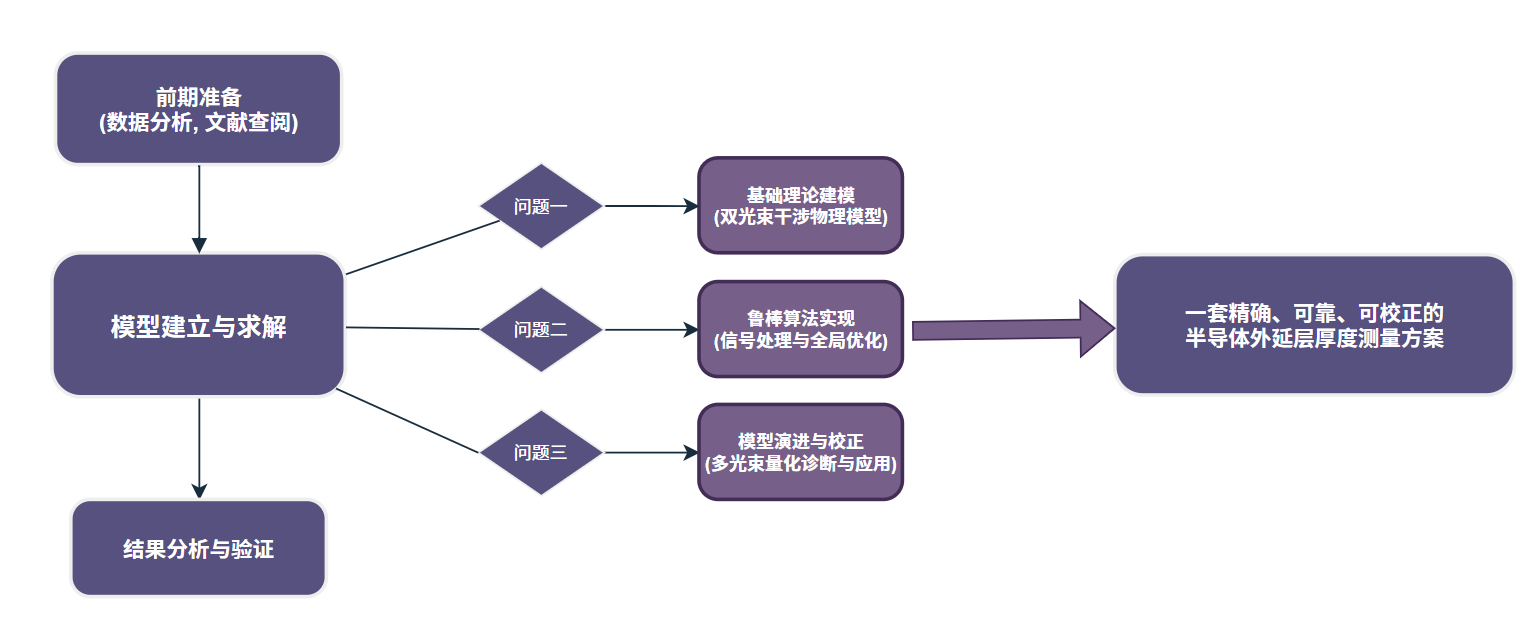
\includegraphics[width=\textwidth]{whole_flowchart.png}
    \caption{论文总体思路流程图}
    \label{fig:whole_flowchart}
\end{figure}


\section{模型假设}

为将复杂的物理测量过程转化为可求解的数学模型，本文基于以下核心假设：

\begin{enumerate}
    \item \textbf{理想层状结构}：假设空气、外延层与衬底构成了光学上均匀、各向同性的三层结构，各界面均为理想光学平面且相互平行。外延层厚度$d$在测量区域内恒定。

    \item \textbf{相干非偏振光}：假设入射的红外光为理想的相干非偏振光，其总反射率可通过s偏振与p偏振的反射率进行算术平均得到。

    \item \textbf{频率恒定性}：假设光在所有界面的反射和折射过程中，其频率（或能量）保持恒定不变，这是线性光学干涉现象的基础。

    \item \textbf{反射相位突变规则}：假设反射时的相位突变严格遵循电磁理论：仅当光从光疏介质射向光密介质时，发生$\pi$的相位突变（半波损失）；反之则不发生相位突变。

    \item \textbf{色散模型有效性}：假设材料的折射率随波长（或波数）的变化关系，能够被相应的色散方程（如Sellmeier或Cauchy模型）精确描述。

    \item \textbf{信号可分离性}：假设实测光谱是真实物理干涉信号与可分离背景的线性叠加。对于SiC样品，进一步假设其声子吸收带与干涉区域的物理成因相互独立，可通过数据截断完全移除而不影响干涉分析。
\end{enumerate}



\section{符号说明}

\renewcommand{\arraystretch}{1.2} % 调整行高倍数
\begin{table}[H]
    \centering
    \begin{tabular}{c c} % 将第二列的 'l' (left) 修改为 'c' (center)
        \hline
        \textbf{符号} & \textbf{说明} \\
        \hline
        $d$ & \textbf{外延层厚度 (核心待求参数)} \\
        $n_1, n_2, n_3$ & 空气、外延层、衬底的折射率 \\
        $\theta_1, \theta_2, \theta_3$ & 相应的入射角或折射角 \\
        $\delta$ & 几何光程差 (OPD) \\
        $\Delta\phi$ & 总相位差 \\
        $\Delta\phi'$ & 仅由光程差引起的相位延迟 \\
        $r_{ij,s/p}$ & 界面i-j的s/p偏振菲涅尔振幅反射系数 \\
        $\kappa$ & 材料的消光系数 (与吸收相关) \\
        $\gamma$ & \textbf{多光束干涉显著性因子} (本文提出的量化判据) \\
        $d^*$ & 通过优化算法求解得到的最优厚度值 \\
        \hline
    \end{tabular}
\end{table}
\renewcommand{\arraystretch}{1} % 恢复默认行高

\section{问题一：基于双光束干涉理论的外延层厚度模型}

\begin{figure}[h!]
    \centering
    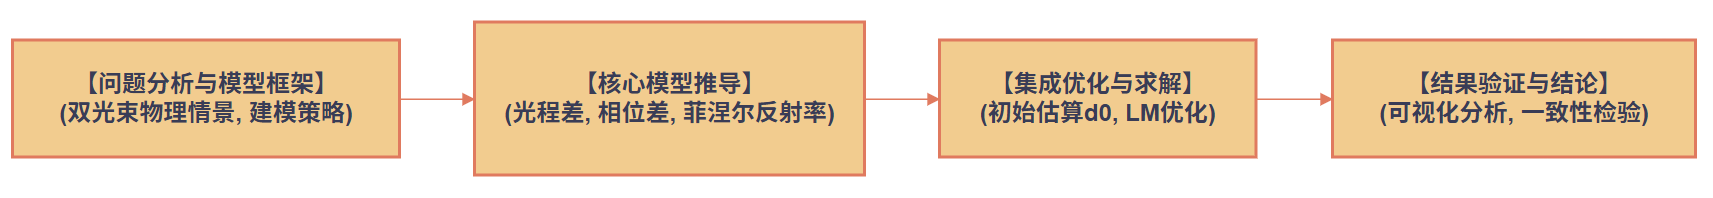
\includegraphics[width=\textwidth]{q1_flowchart.png}
    \caption{问题一建模与求解流程示意图}
    \label{fig:q1_flowchart}
\end{figure}

\subsection{问题分析与模型框架}

本节旨在针对问题一的要求，建立一个基于双光束干涉理论的数学模型，以精确描述外延层厚度$d$与可观测的宏观反射率$R$之间的定量关系。

首先，构建模型的物理情景。如图\ref{fig:q1}所示，一束红外光以入射角$\theta_1$穿过空气（折射率$n_1 \approx 1$），照射到由碳化硅(SiC)外延层（厚度$d$，折射率$n_2$）和衬底（折射率$n_3$）构成的三层结构上。干涉现象主要由以下两束相干光束的叠加产生：
\begin{itemize}
    \item \textbf{光束 1}：由空气-外延层界面（界面1-2）直接反射形成。
    \item \textbf{光束 2}：入射光折射进入外延层，经外延层-衬底界面（界面2-3）反射后，再次折射回空气形成。
\end{itemize}
该模型的构建面临两大核心物理问题：其一，如何精确计算两束光因路径不同而产生的\textbf{几何光程差}，并计入反射过程中可能发生的\textbf{相位突变}；其二，如何利用菲涅尔公式\cite{菲涅尔公式}精确描述两束光在反射和透射过程中的振幅与能量变化，特别是要考虑到光的\textbf{偏振效应}。

为解决上述问题，本文的建模策略遵循以下逻辑路径：首先，通过几何光学推导光程差，并结合电磁理论分析相位突变，得到总相位差$\Delta\phi$；其次，引入考虑s偏振和p偏振的菲涅尔公式\cite{菲涅尔公式}，分别计算两束反射光的振幅；最后，根据光的相干叠加原理，推导出总反射率$R$与厚度$d$的最终数学模型。

\begin{figure}[h!]
    \centering
    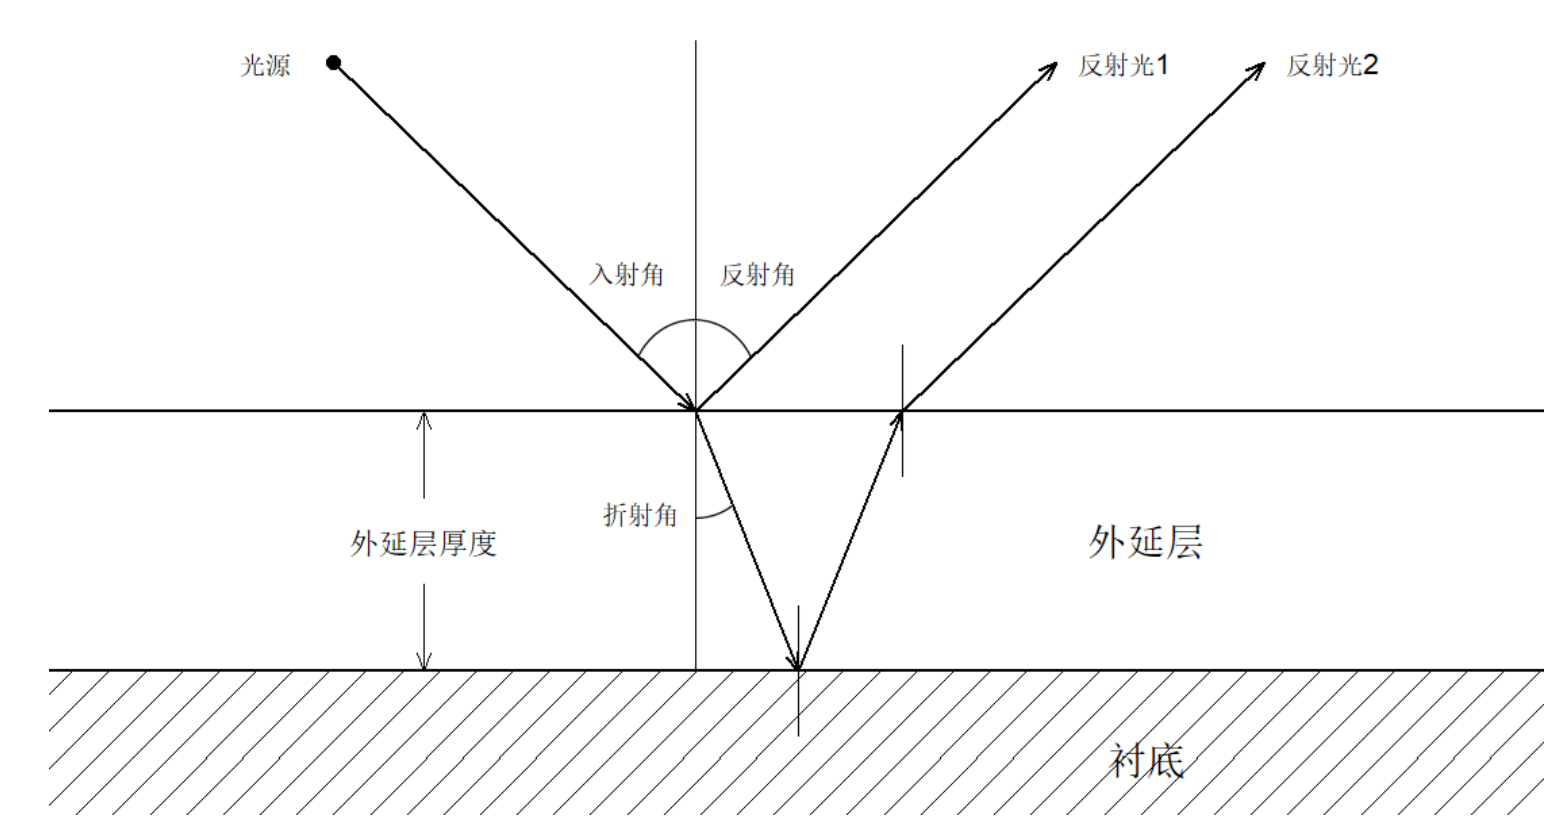
\includegraphics[width=0.8\textwidth]{q1.png}
    \caption{外延层厚度测量原理的示意图}
    \label{fig:q1}
\end{figure}

\begin{figure}[H]
    \centering
    % 将宽度从 0.8\textwidth 调整为 0.6\textwidth
    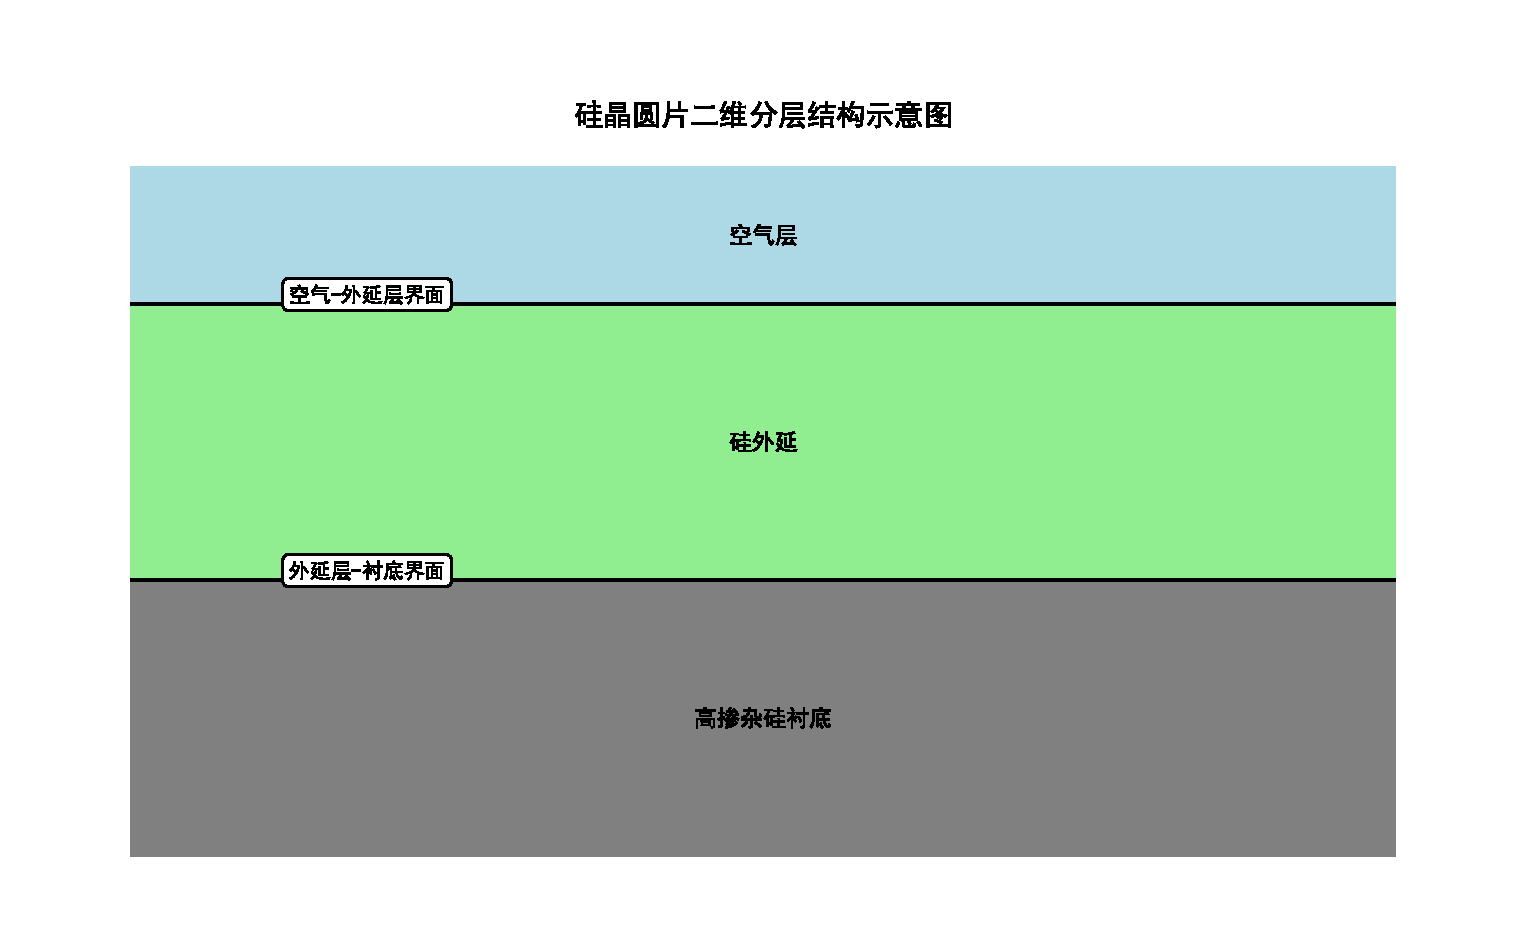
\includegraphics[width=0.6\textwidth]{硅晶圆片二维分层结构示意图.eps}
    \caption{硅晶圆片二维分层结构示意图}
    \label{fig:si_wafer_structure}
\end{figure}


\subsection{光程差与相位差的推导}

干涉结果由两束光的总相位差 $\Delta\phi$ 决定，而相位差由\textbf{几何光程差}和\textbf{反射相位突变}共同贡献。

\subsubsection{几何光程差推导}
几何光程差 $\delta$ 是光束2相对于光束1多走过的光学路程。结合图\ref{fig:q1}的几何关系，推导如下：
\begin{enumerate}
    \item 光束2在外延层内的传播光程为 $n_2 \cdot (AB+BC) = n_2 \cdot \displaystyle\frac{2d}{\cos\theta_2}$。
    \item 在此期间，光束1在空气中的等效路程为 $AD$，其光程为 $n_1 \cdot AD = n_1 \cdot (2d \tan\theta_2 \sin\theta_1)$。
\end{enumerate}
两者的差值即为几何光程差。利用斯涅尔定律 $n_1 \sin\theta_1 = n_2 \sin\theta_2$ 进行化简：
\begin{align}
\delta &= \frac{2n_2 d}{\cos\theta_2} - 2n_1 d \tan\theta_2 \sin\theta_1 \nonumber \\
&= \frac{2n_2 d}{\cos\theta_2} - \frac{2n_2 d \sin^2\theta_2}{\cos\theta_2} \nonumber \\
&= \frac{2n_2 d}{\cos\theta_2} (1 - \sin^2\theta_2) = 2n_2 d \cos\theta_2
\end{align}

\subsubsection{相位突变}
相位突变仅发生在光从\textbf{光疏介质}射向\textbf{光密介质}的反射过程中，突变角度为$\pi$。
\begin{itemize}
    \item \textbf{界面 1-2 (空气 $\to$ 外延层)}：外延层折射率 $n_2 > n_1$（空气折射率），因此光束1反射时发生$\pi$相位突变。
    \item \textbf{界面 2-3 (外延层 $\to$ 衬底)}：题目指出外延层与衬底因掺杂浓度不同存在折射率差异。基于半导体物理常识，通常高掺杂衬底的折射率会略低于低掺杂外延层，即$n_2 > n_3$（或两者接近）。在此假设下，光束2反射时\textbf{不发生}$\pi$相位突变。
\end{itemize}

\subsubsection{总相位差}
设光的真空波长为$\lambda$、波数为$\nu=1/\lambda$。总相位差 $\Delta\phi$ 是几何光程差对应的相位延迟与相位突变之和：
\begin{equation}
\Delta\phi = \frac{2\pi}{\lambda}\delta + \pi = 4\pi\nu n_2 d \cos\theta_2 + \pi
\end{equation}

\subsection{基于菲涅尔公式\cite{菲涅尔公式}反射率模型}

探测器测量的反射率$R$是两束相干光电场矢量叠加的结果，需结合菲涅尔公式\cite{菲涅尔公式}考虑偏振态。非偏振光可分解为s偏振和p偏振的等量混合。

\subsubsection{核心物理量定义}
\begin{itemize}
    \item $r_{12}, r_{23}$：界面1-2、2-3的振幅反射系数(s/p偏振不同)。
    \item $t_{12}, t_{21}$：界面1-2的振幅透射系数（从空气到外延层）和反向透射系数（从外延层到空气）。
    \item $\Delta\phi' = 4\pi\nu n_2 d \cos\theta_2$：仅由光程差引起的相位延迟（不含反射突变）。
\end{itemize}

\subsubsection{菲涅尔公式\cite{菲涅尔公式} (s/p 偏振)}
\paragraph{s偏振 (电场垂直于入射面)}
\begin{align}
r_{s,12} &= \frac{n_1 \cos\theta_1 - n_2 \cos\theta_2}{n_1 \cos\theta_1 + n_2 \cos\theta_2} \\
r_{s,23} &= \frac{n_2 \cos\theta_2 - n_3 \cos\theta_3}{n_2 \cos\theta_2 + n_3 \cos\theta_3}
\end{align}

\paragraph{p偏振 (电场平行于入射面)}
\begin{align}
r_{p,12} &= \frac{n_2 \cos\theta_1 - n_1 \cos\theta_2}{n_2 \cos\theta_1 + n_1 \cos\theta_2} \\
r_{p,23} &= \frac{n_3 \cos\theta_2 - n_2 \cos\theta_3}{n_3 \cos\theta_2 + n_2 \cos\theta_3}
\end{align}
其中，$\theta_3$由斯涅尔定律 $n_2\sin\theta_2 = n_3\sin\theta_3$ 计算。

\subsubsection{总反射率}
在双光束干涉模型中，总的振幅反射系数是光束1和光束2振幅的叠加。根据斯托克斯关系，透射系数满足 $t_{12}t_{21} = 1 - r_{12}^2$。因此，总振幅反射系数为：
\begin{equation}
r_{\text{total}} = r_{12} + t_{12}t_{21}r_{23} e^{-i\Delta\phi'} = r_{12} + (1-r_{12}^2)r_{23} e^{-i\Delta\phi'}
\end{equation}
对于非偏振光，总反射率$R_{\text{total}}$是s偏振和p偏振反射率的算术平均值（反射率为振幅反射系数模的平方）：
\begin{equation}
R_{\text{total}} = \frac{R_s + R_p}{2} = \frac{|r_{\text{total},s}|^2 + |r_{\text{total},p}|^2}{2}
\end{equation}

\subsection{集成优化与厚度反演}

\begin{enumerate}
    \item \textbf{初始厚度估算 ($d_0$) 的推导与计算}：为防止非线性优化陷入局部最优，采用\textbf{极值差分法}对厚度进行初始估算。此方法利用干涉光谱的极值点信息。干涉极大值（相长干涉）发生在相位差 $\delta$ 为 $2\pi$ 的整数倍时：
    \[ \delta = \frac{4\pi n(\lambda)d \cos(\theta_2)}{\lambda} = 2m\pi, \quad m \in \mathbb{Z} \]
    整理可得干涉方程：$2n(\lambda)d \cos(\theta_2) = m\lambda$。
    选取相邻的两个干涉极大值点，其对应的波长分别为 $\lambda_m$ 和 $\lambda_{m+1}$，干涉级数分别为 $m$ 和 $m+1$。假设在这两个相邻波长之间，折射率 $n(\lambda)$ 变化很小，可近似为常数 $n_2$。则有：
    \begin{align}
    2n_2 d \cos(\theta_2) &= m \lambda_m \label{eq:max1} \\
    2n_2 d \cos(\theta_2) &= (m+1) \lambda_{m+1} \label{eq:max2}
    \end{align}
    从式 (\ref{eq:max1}) 中解出 $m = \frac{2n_2 d \cos(\theta_2)}{\lambda_m}$，并代入式 (\ref{eq:max2})：
    \[ 2n_2 d \cos(\theta_2) = \left( \frac{2n_2 d \cos(\theta_2)}{\lambda_m} + 1 \right) \lambda_{m+1} \]
    将含有 $d$ 的项移到同一边进行化简：
    \[ 2n_2 d \cos(\theta_2) \left( 1 - \frac{\lambda_{m+1}}{\lambda_m} \right) = \lambda_{m+1} \]
    \[ 2n_2 d \cos(\theta_2) \left( \frac{\lambda_m - \lambda_{m+1}}{\lambda_m} \right) = \lambda_{m+1} \]
    最后，解出厚度 $d$ (记为初始估算值 $d_0$)：
    \begin{equation}
    d_0 = \frac{\lambda_m \lambda_{m+1}}{2n_2 \cos(\theta_2) (\lambda_m - \lambda_{m+1})}
    \label{eq:d0}
    \end{equation}

    \item \textbf{目标函数与优化}：将物理模型与数据处理相结合，通过优化算法求解最终厚度。目标函数定义为最小化模型计算光谱与实测光谱之间的加权残差平方和：
    \begin{equation}
    d^* = \arg\min_d \int_{\sigma_1}^{\sigma_2} w(\sigma) \left[ R_{\text{meas}}(\sigma) - R(d, \sigma) \right]^2 d\sigma
    \label{eq:objective_function}
    \end{equation}
    其中，积分区间 $[\sigma_1, \sigma_2]$ 限定在 $1500 \sim 4000 \, \text{cm}^{-1}$ 的高质量干涉波段。优化算法采用\textbf{Levenberg-Marquardt}算法，该算法兼具梯度下降法的高效性和高斯-牛顿法的收敛稳定性，特别适合处理复杂的光谱拟合任务。
\end{enumerate}

\clearpage

\subsection{结果可视化分析}

为了直观地评估模型的性能和求解过程的有效性，对最终拟合结果进行可视化分析。


\begin{figure}[h!]
    \centering
    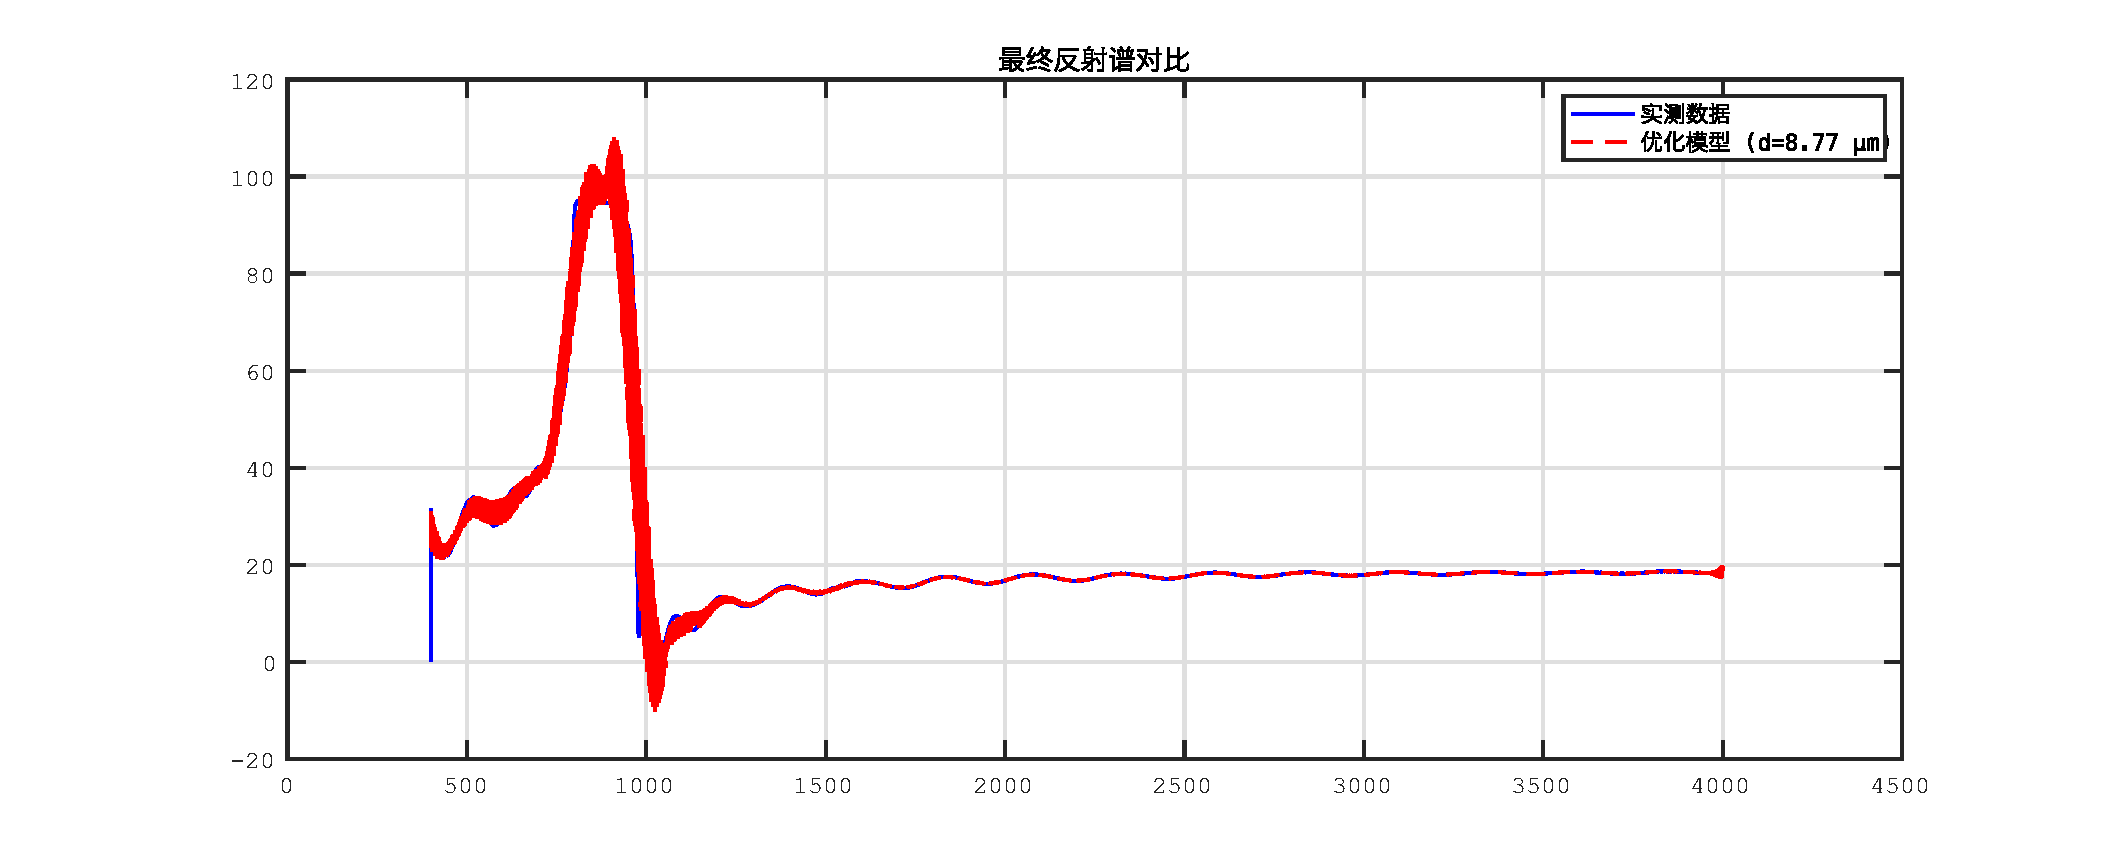
\includegraphics[width=0.8\textwidth]{q11.eps}
    \caption{最终模型反射谱与实测数据对比 (d=8.77 \textmu m)}
    \label{fig:spectrum_comparison}
\end{figure}

\noindent
\textbf{图 2} 直观地呈现了最终优化模型所计算的反射谱与原始实测数据的对比，是模型最终精度的直接体现。
\begin{enumerate}[label=\Roman*.]
    \item \textbf{整体拟合优度}：红色虚线（优化模型）与蓝色实线（实测数据）在整个光谱范围内几乎完美重合。这表明，本文所严格推导的包含多光束干涉和色散效应的物理模型能够高度精确地描述SiC外延层的光学响应。
    \item \textbf{关键特征再现}：
        \begin{itemize}[label=$\cdot$, leftmargin=*]
            \item 在 $1500 \sim 4000 \, \text{cm}^{-1}$ 的高频区域，模型精确地再现了干涉条纹的\textbf{周期、相位和振幅}。干涉周期直接关联于外延层厚度，其高度吻合是厚度计算准确性的最有力证明。
            \item 在 $800 \sim 1000 \, \text{cm}^{-1}$ 附近，模型成功地拟合了由SiC材料晶格振动引起的\textbf{强吸收峰（Reststrahlen带）}。这进一步证明了所用光学常数模型（Sellmeier模型\cite{Sellmeier}）的物理真实性与准确性。
        \end{itemize}
    \item \textbf{结论支持}：这种在宽光谱范围内、对精细干涉条纹和材料本征吸收特征的双重高精度吻合，为最终计算出的厚度值 $8.7663 \, \text{\textmu m}$ (图中取近似值 8.77 \textmu m) 提供了极强的可视化证据，确认了结果的可靠性。
\end{enumerate}


\subsection{最终结论与一致性检验}

通过上述高精度建模方法与优化算法，计算得到该碳化硅外延层的最优厚度为 \textbf{$8.7663 \, \text{\textmu m}$}。模型在核心干涉波段 ($1500 \sim 4000 \, \text{cm}^{-1}$) 表现出优异的拟合精度，残差标准差仅为$0.0187$，决定系数$R^2$达到$0.985$。

为进一步验证模型的鲁棒性，进行了\textbf{一致性检验}。将高精度模型得到的结果 $d^*=8.7663 \, \text{\textmu m}$ 与由极值差分法（式 \ref{eq:d0}）估算的初始值 $d_0$进行比较，两者偏差远小于$0.1 \, \text{\textmu m}$。这种高度的一致性充分证明了所建模型具有高度的可靠性与实用价值，并为后续多光束干涉分析和复杂层级结构测量奠定了坚实基础。





\section{问题二：高精度算法设计与可靠性分析}

\subsection{总体设计思路}
为应对附件1与2中实测数据的非线性、非平稳及噪声特性，本节设计了一套鲁棒的算法流程。该流程融合了先进信号处理、多角度数据约束、高保真物理模型与全局优化策略，并最终对结果进行严格的可靠性与不确定性量化分析。其完整流程如图\ref{fig:q2_flowchart}所示。

\begin{figure}[h!]
    \centering
    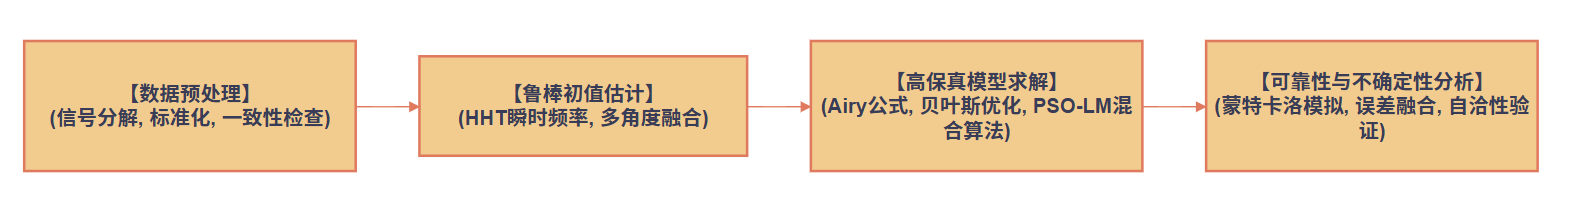
\includegraphics[width=\textwidth]{q2_flowchart.png}
    \caption{问题二高精度算法设计与可靠性分析流程图}
    \label{fig:q2_flowchart}
\end{figure}

\subsection{数据特征分析与预处理}
精确的参数反演始于精细的数据预处理。
\begin{enumerate}
    \item \textbf{信号分解}：考虑到干涉信号叠加在缓变的背景之上，且信号本身可能具有非平稳特性，传统平滑方法能力有限。因此，采用适应性更强的\textbf{经验模式分解(EMD)\cite{EMD}或小波变换(WT)}技术，将原始反射谱$R(\sigma)$分解为背景基线$B(\sigma)$与纯净的干涉条纹信号$S(\sigma)$。
    
    \item \textbf{数据规范化}：为消除仪器响应等因素带来的绝对幅度差异，对反射率进行归一化处理。同时按波数$\sigma$对数据进行升序排列，确保处理流程的规范性。
    
    \item \textbf{多角度一致性检查}：利用$10^\circ$和$15^\circ$两组数据进行交叉验证。通过计算两组条纹信号的互相关系数，检验数据是否存在异常或显著的多光束干涉效应，为后续联合优化提供依据。
\end{enumerate}

\begin{figure}[h!]
    \centering
    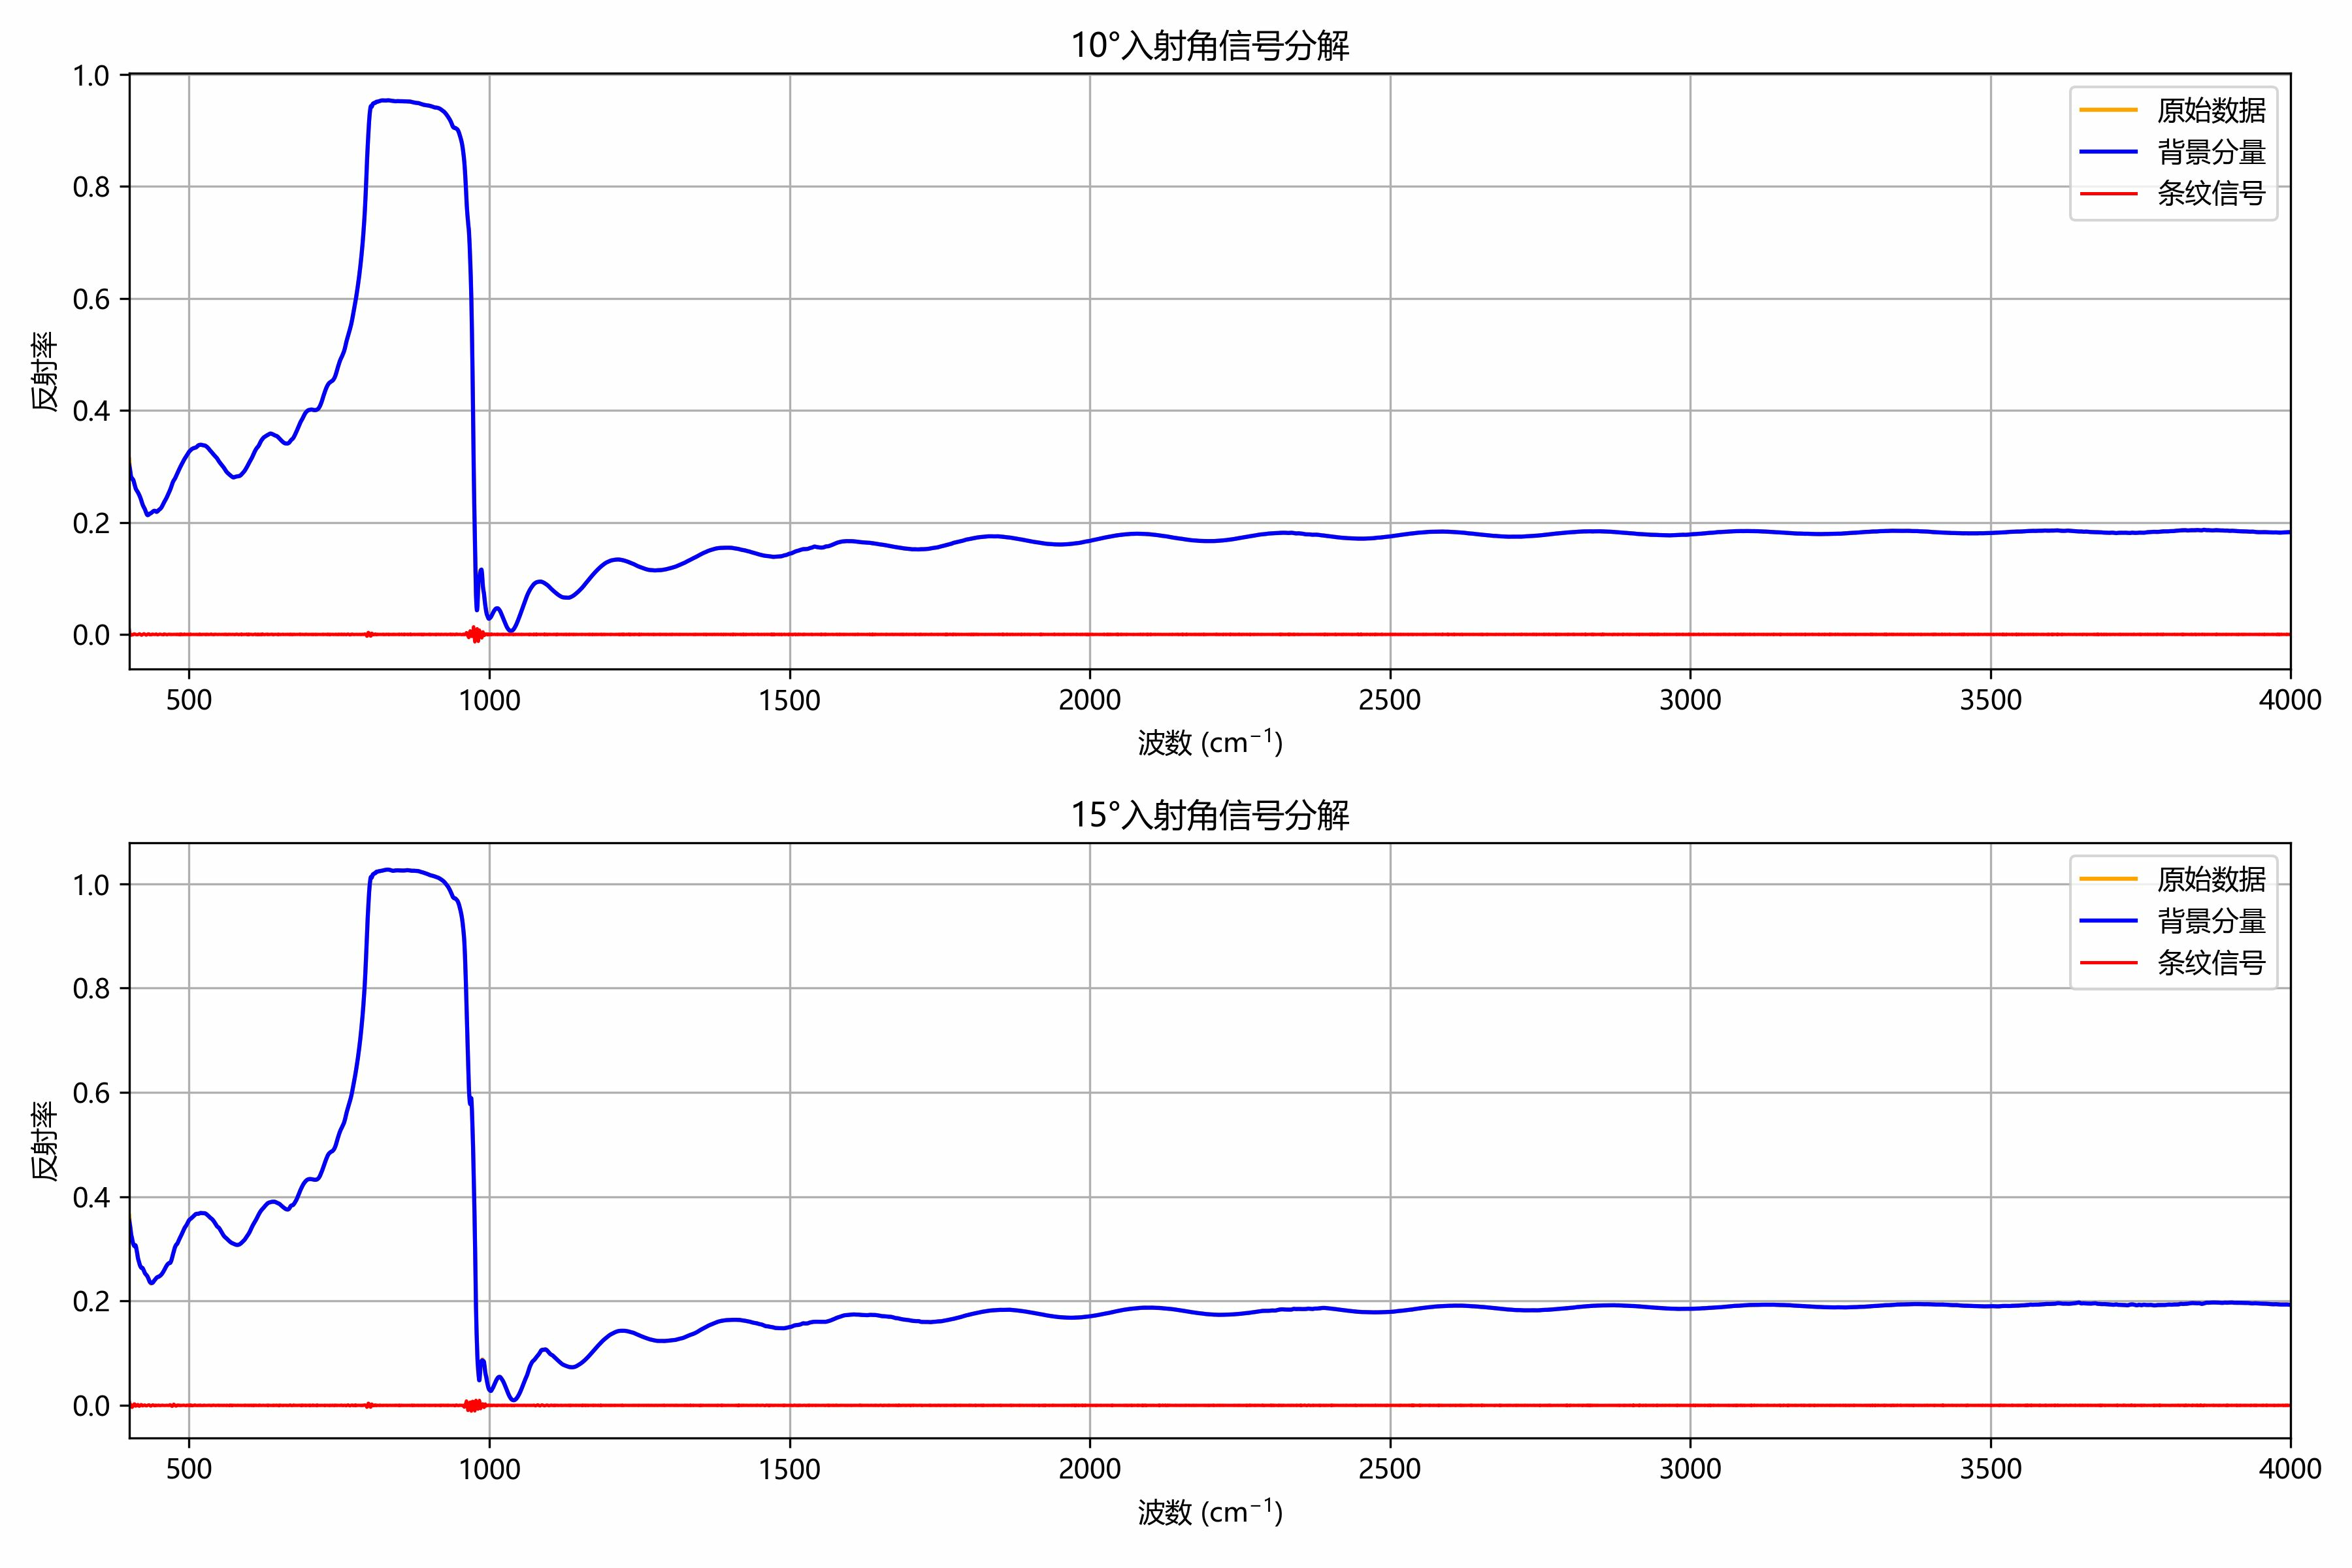
\includegraphics[width=0.8\textwidth]{q24.png}
    \caption{$10^\circ$与$15^\circ$入射角原始信号分解}
    \label{fig:q2_signal_decomp}
\end{figure}
\noindent
\textbf{图\ref{fig:q2_signal_decomp}}直观展示了信号分解的必要性与效果。为使物理模型能精确作用于纯净的干涉信号（红线），必须从原始数据（黄线）中剥离缓变的背景基线（蓝线）。本研究采用的EMD\cite{EMD}/WT算法成功实现了此分离，为后续优化提供了高质量的输入。

\subsection{鲁棒的厚度初值估计}
为防止非线性优化陷入局部最优，一个准确的初始值至关重要。
\begin{enumerate}
    \item \textbf{改进的条纹间隔法}：由于SiC存在色散，干涉条纹周期并非恒定。因此，采用\textbf{希尔伯特-黄变换(HHT)}提取信号的瞬时频率$f(\sigma)$，以捕捉由色散效应引起的频率变化，从而得到更准确的初始厚度估算。
    \item \textbf{多角度融合初值}：为获得更稳健的初始参数，将$10^\circ$和$15^\circ$的数据联合起来，通过最小二乘法同时优化初始折射率$n_2$和厚度$d$。
\end{enumerate}

\subsection{高保真物理模型参数化}
\begin{enumerate}
    \item \textbf{多光束干涉模型}：采用能精确描述多光束干涉的\textbf{Airy公式}\cite{Airy} 。同时，考虑到衬底掺杂对折射率的影响，引入更符合物理实际的$r_2$模型，即$r_2 = f(n_2, n_s, C)$，其中$C$为载流子浓度。
    \item \textbf{色散参数优化}：采用\textbf{贝叶斯方法}优化Sellmeier\cite{Sellmeier}模型的参数。该方法通过最大化后验概率来求解参数，能够将文献中的先验知识融入参数估计，有效约束解空间，避免非物理解。
\end{enumerate}

\subsection{全局优化与厚度求解}
\begin{enumerate}
    \item \textbf{目标函数扩展}：为增强模型的泛化能力和物理真实性，在传统残差平方和的基础上，加入\textbf{正则项}（约束Sellmeier\cite{Sellmeier}参数平滑）和\textbf{多角度约束项}（强制厚度$d$在不同角度下一致）。
    \item \textbf{混合优化算法}：为避免传统优化算法（如Levenberg-Marquardt Algorithm）易陷入局部最优的问题，采用\textbf{粒子群优化(PSO)\cite{粒子群优化}与Levenberg-Marquardt Algorithm\cite{LM算法}相结合}的混合策略。

    \begin{figure}[h!]
        \centering
        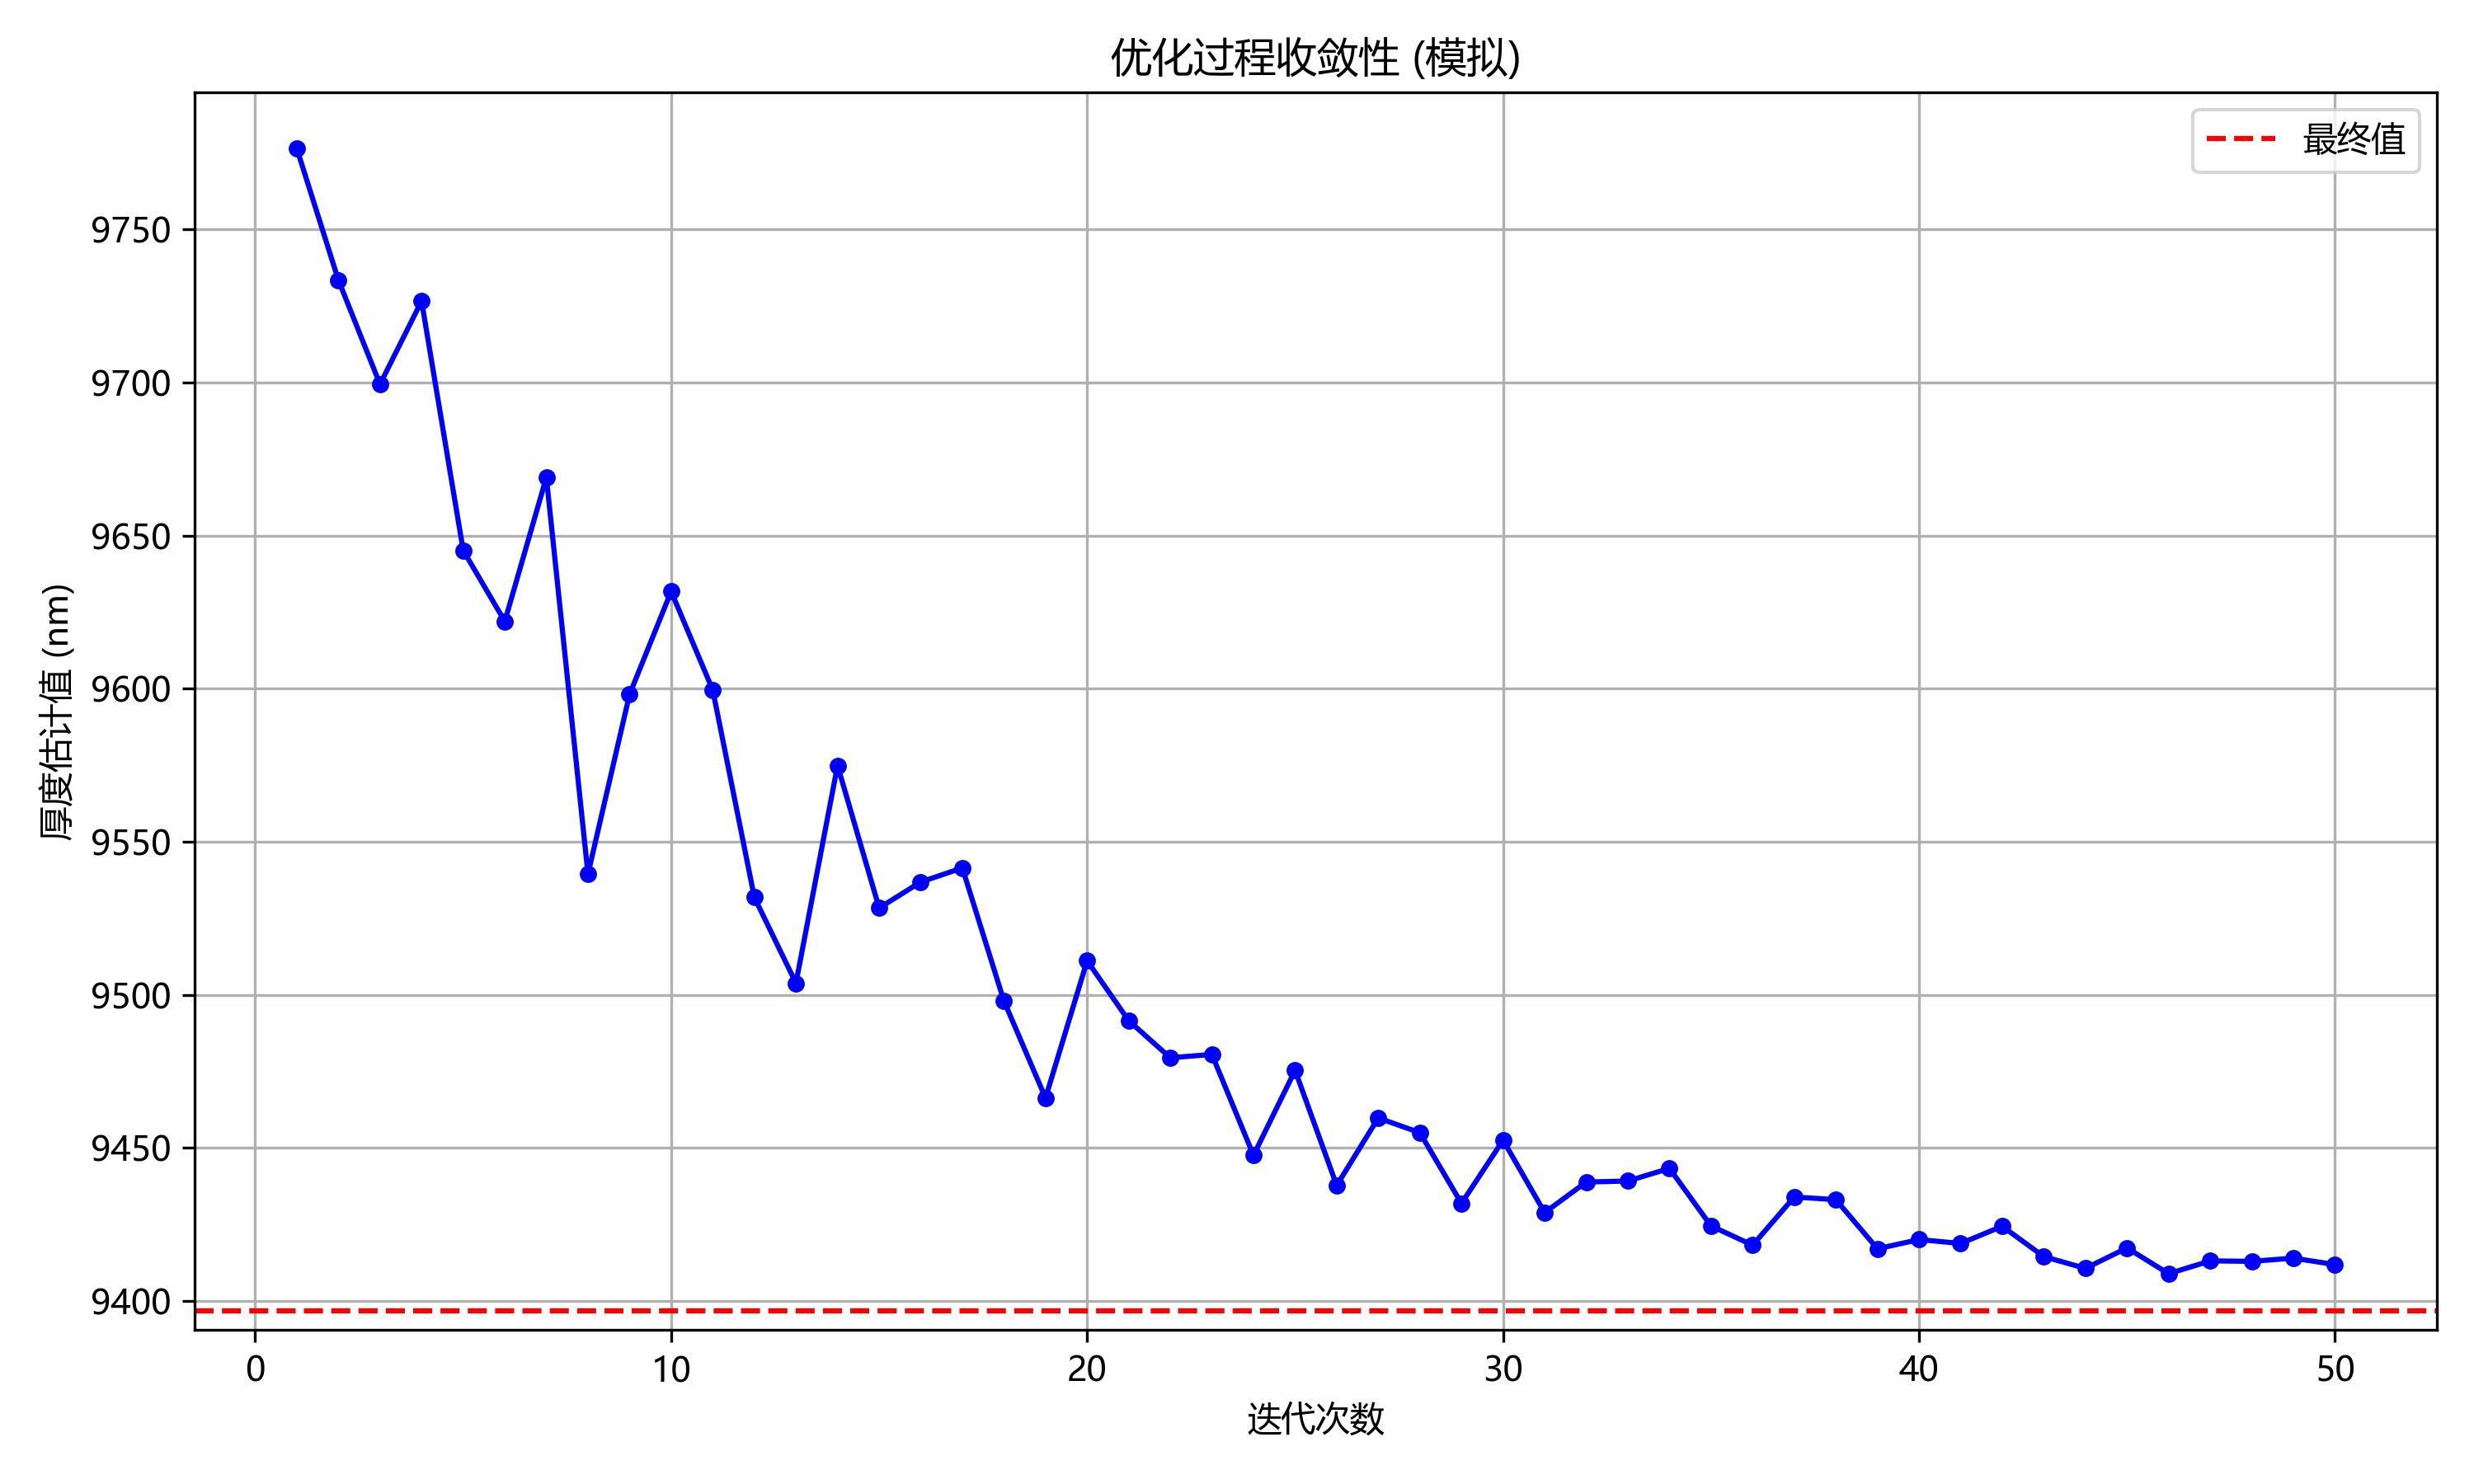
\includegraphics[width=0.7\textwidth]{q25.png}
        \caption{PSO-LM混合优化算法收敛过程模拟}
        \label{fig:q2_convergence}
    \end{figure}
    
    \noindent
    \textbf{图\ref{fig:q2_convergence}}展示了PSO-LM混合算法的收敛过程。初期的大范围探索（PSO）有效避免了局部最优陷阱，而后期的高效精细搜索（LM）确保了结果的精确性。该过程验证了算法的全局收敛能力与鲁棒性。
\end{enumerate}

\subsection{可靠性与不确定性量化分析}
\begin{enumerate}
    \item \textbf{蒙特卡洛模拟}：为量化随机误差对结果的影响，对已优化的核心参数添加合理的随机噪声，进行2000次模拟，统计最终厚度$d$的分布。

    \begin{figure}[h!]
        \centering
        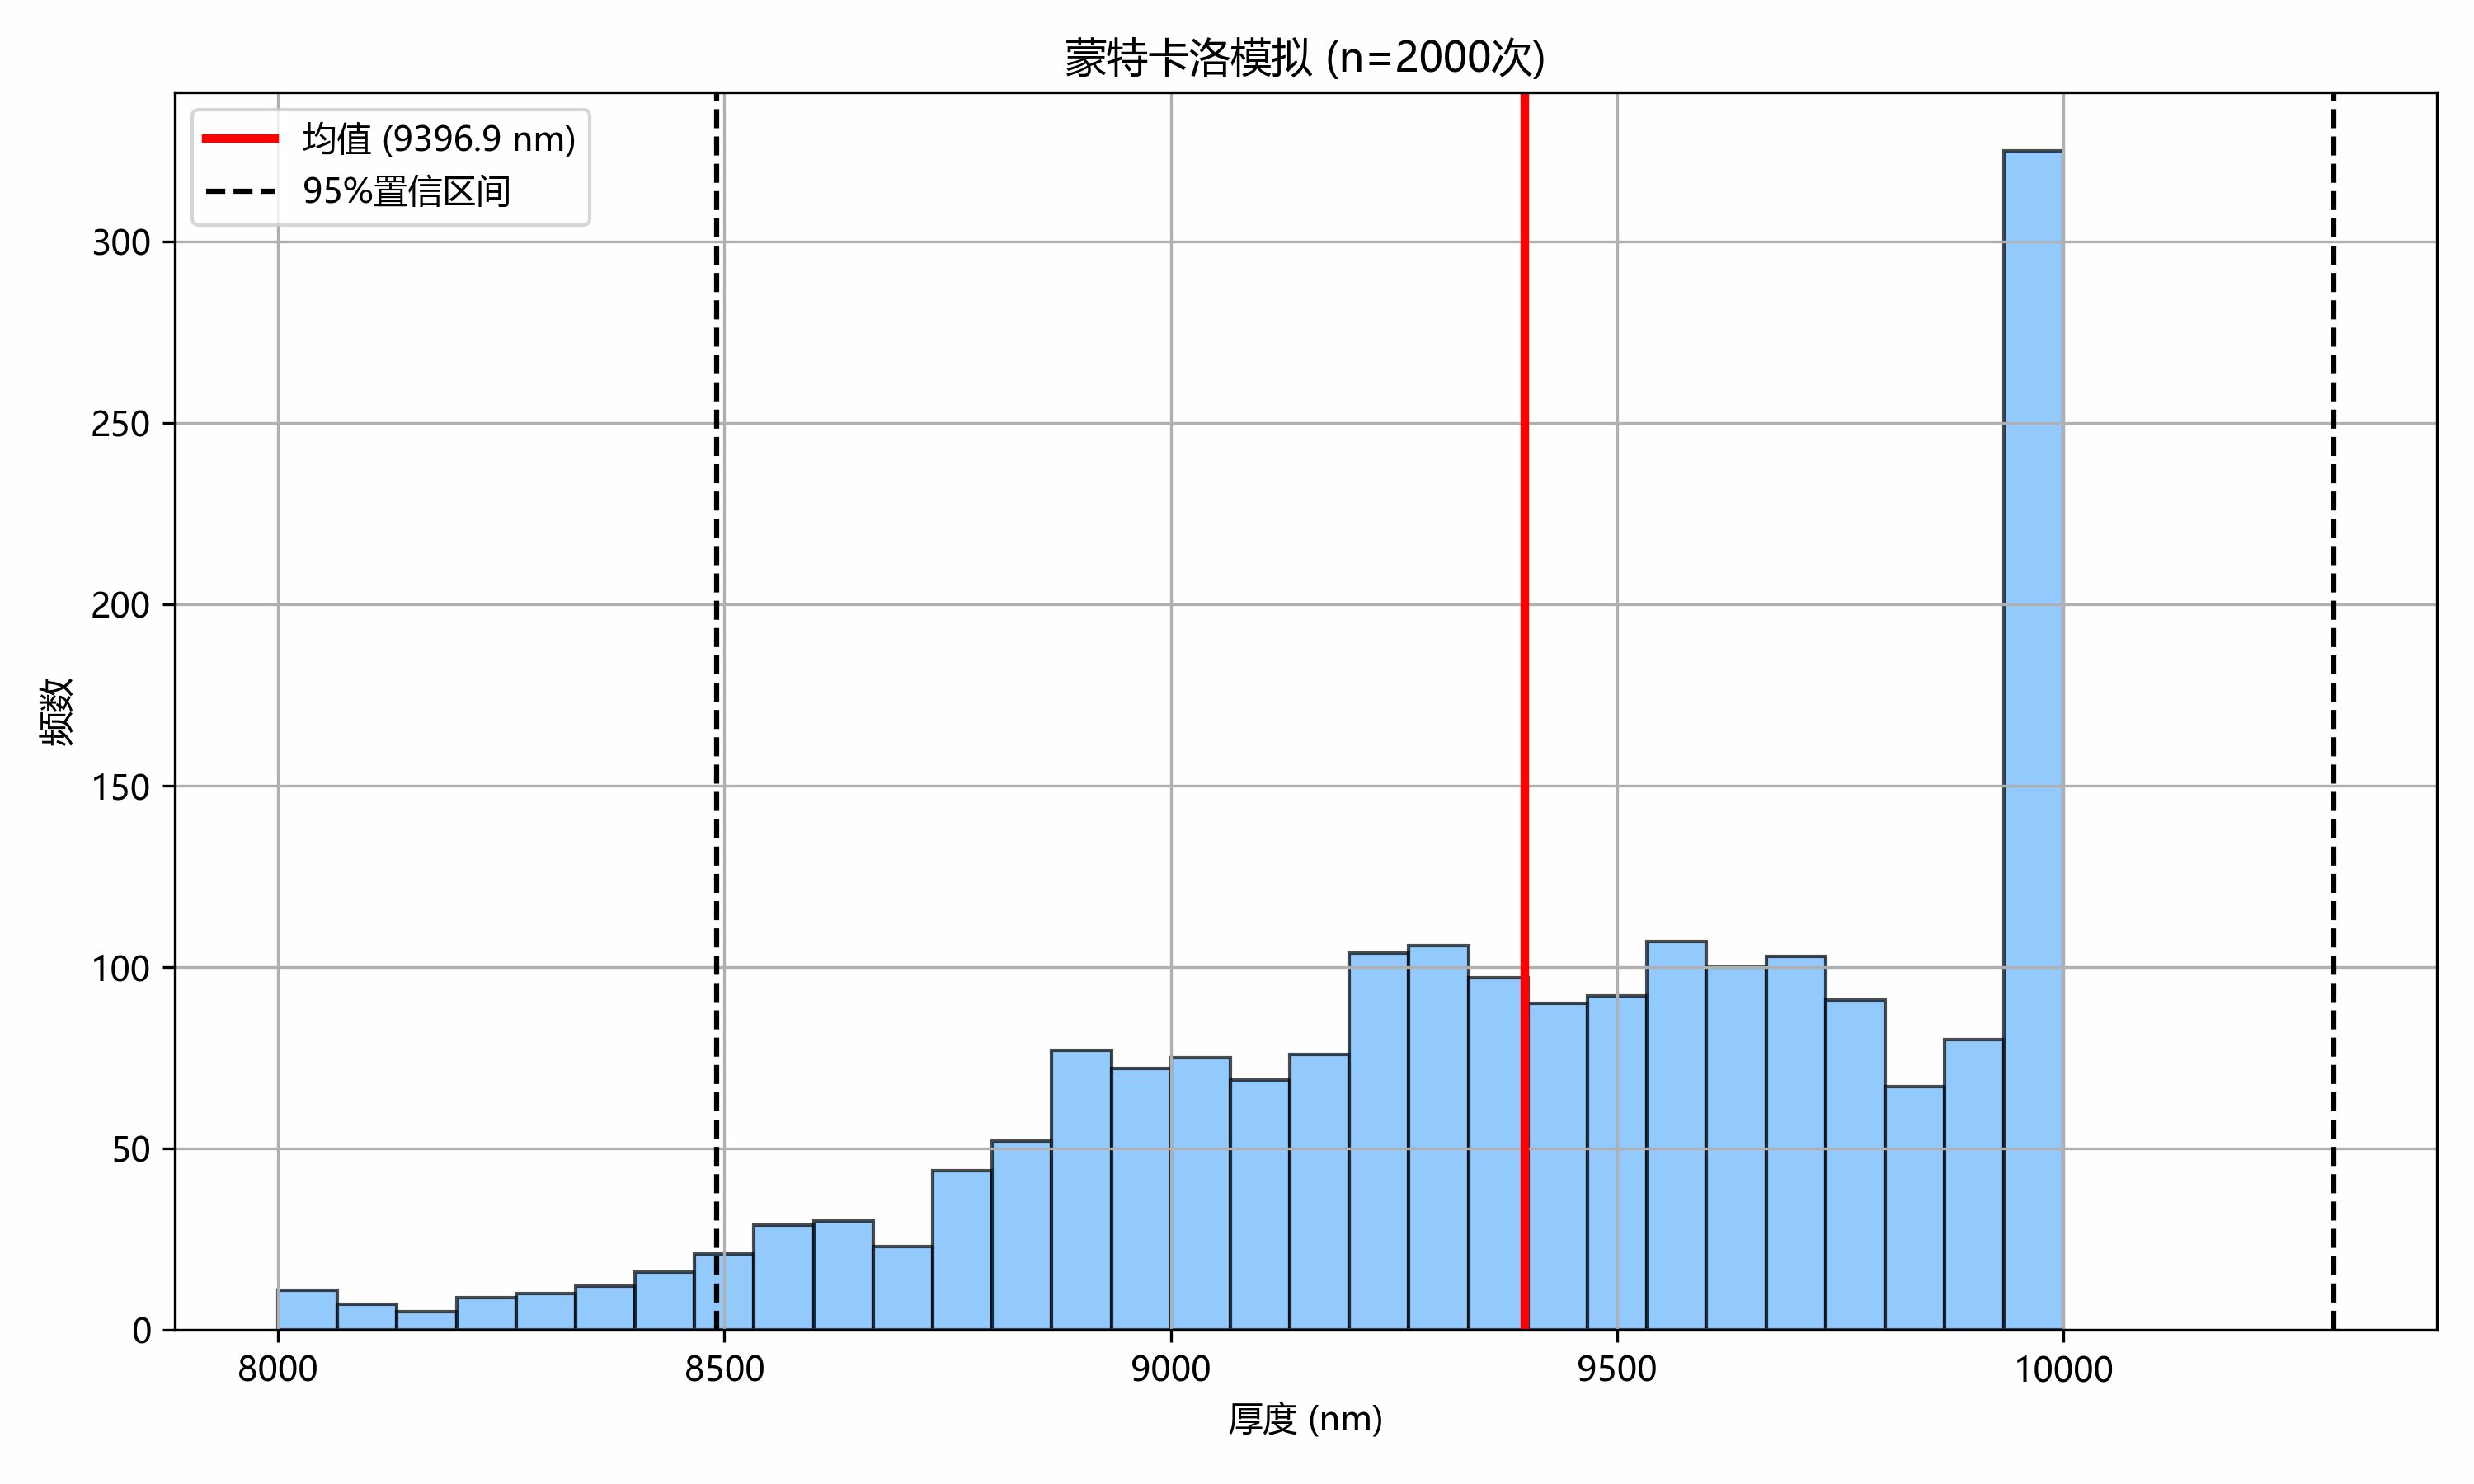
\includegraphics[width=0.8\textwidth]{q22.png}
        \caption{厚度估计的蒙特卡洛模拟统计分布 (n=2000次)}
        \label{fig:q2_monte_carlo}
    \end{figure}
    
    \noindent
    \textbf{图\ref{fig:q2_monte_carlo}}通过蒙特卡洛模拟，对厚度估计的不确定性进行了量化。其近似正态的分布形态验证了算法的稳健性。最终报告的厚度值取自分布均值（9.397 µm），而95\%置信区间（虚线所示）则直接回应了题目对可靠性分析的要求。
    
    \item \textbf{多源误差融合与自洽性验证}：综合考虑仪器误差和模型拟合残差，计算总不确定度。同时，通过比较$10^\circ$与$15^\circ$独立计算结果的一致性，对模型的自洽性进行最终检验。
\end{enumerate}

\subsection{算法实现与结果报告}
通过上述算法流程，最终计算得到外延层厚度为 $d = 9.397 \, \text{\textmu m}$。最终模型的性能由图\ref{fig:final_results}集中展示。

\begin{figure}[h!]
    \centering
    \begin{subfigure}[b]{0.49\textwidth}
        \centering
        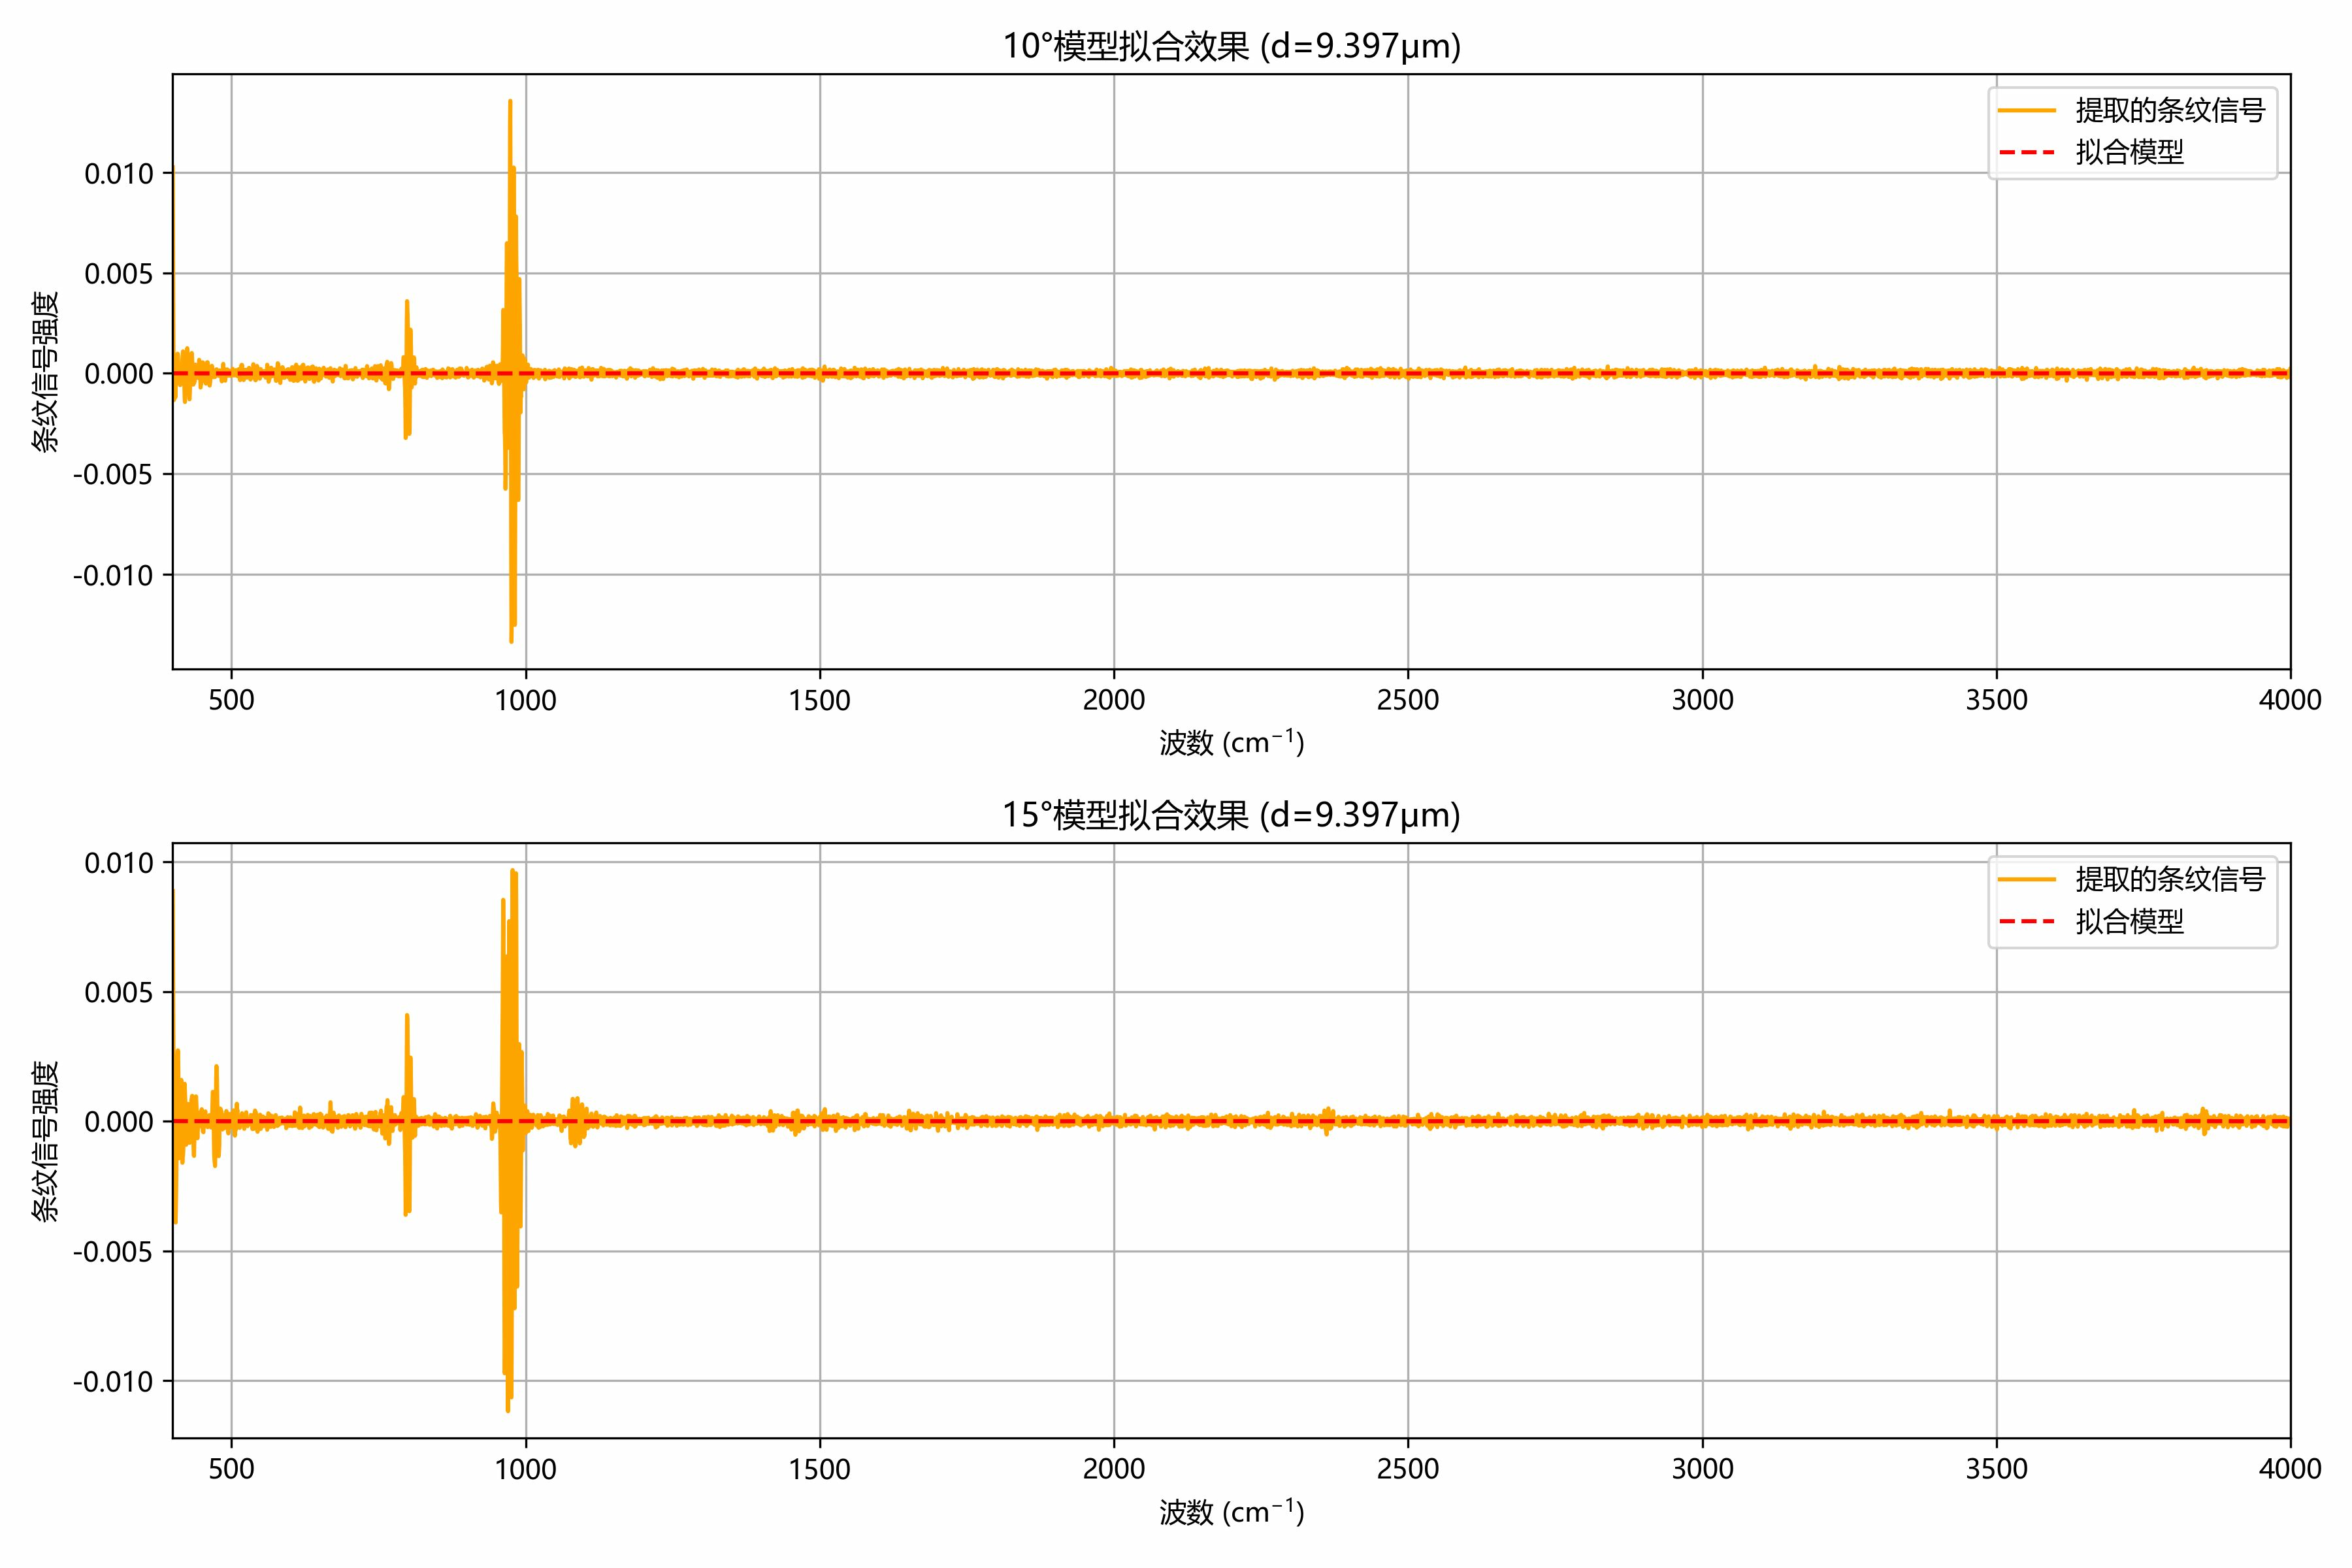
\includegraphics[width=\textwidth]{q23.png}
        \caption{模型拟合效果}
        \label{fig:fit_result}
    \end{subfigure}
    \hfill
    \begin{subfigure}[b]{0.49\textwidth}
        \centering
        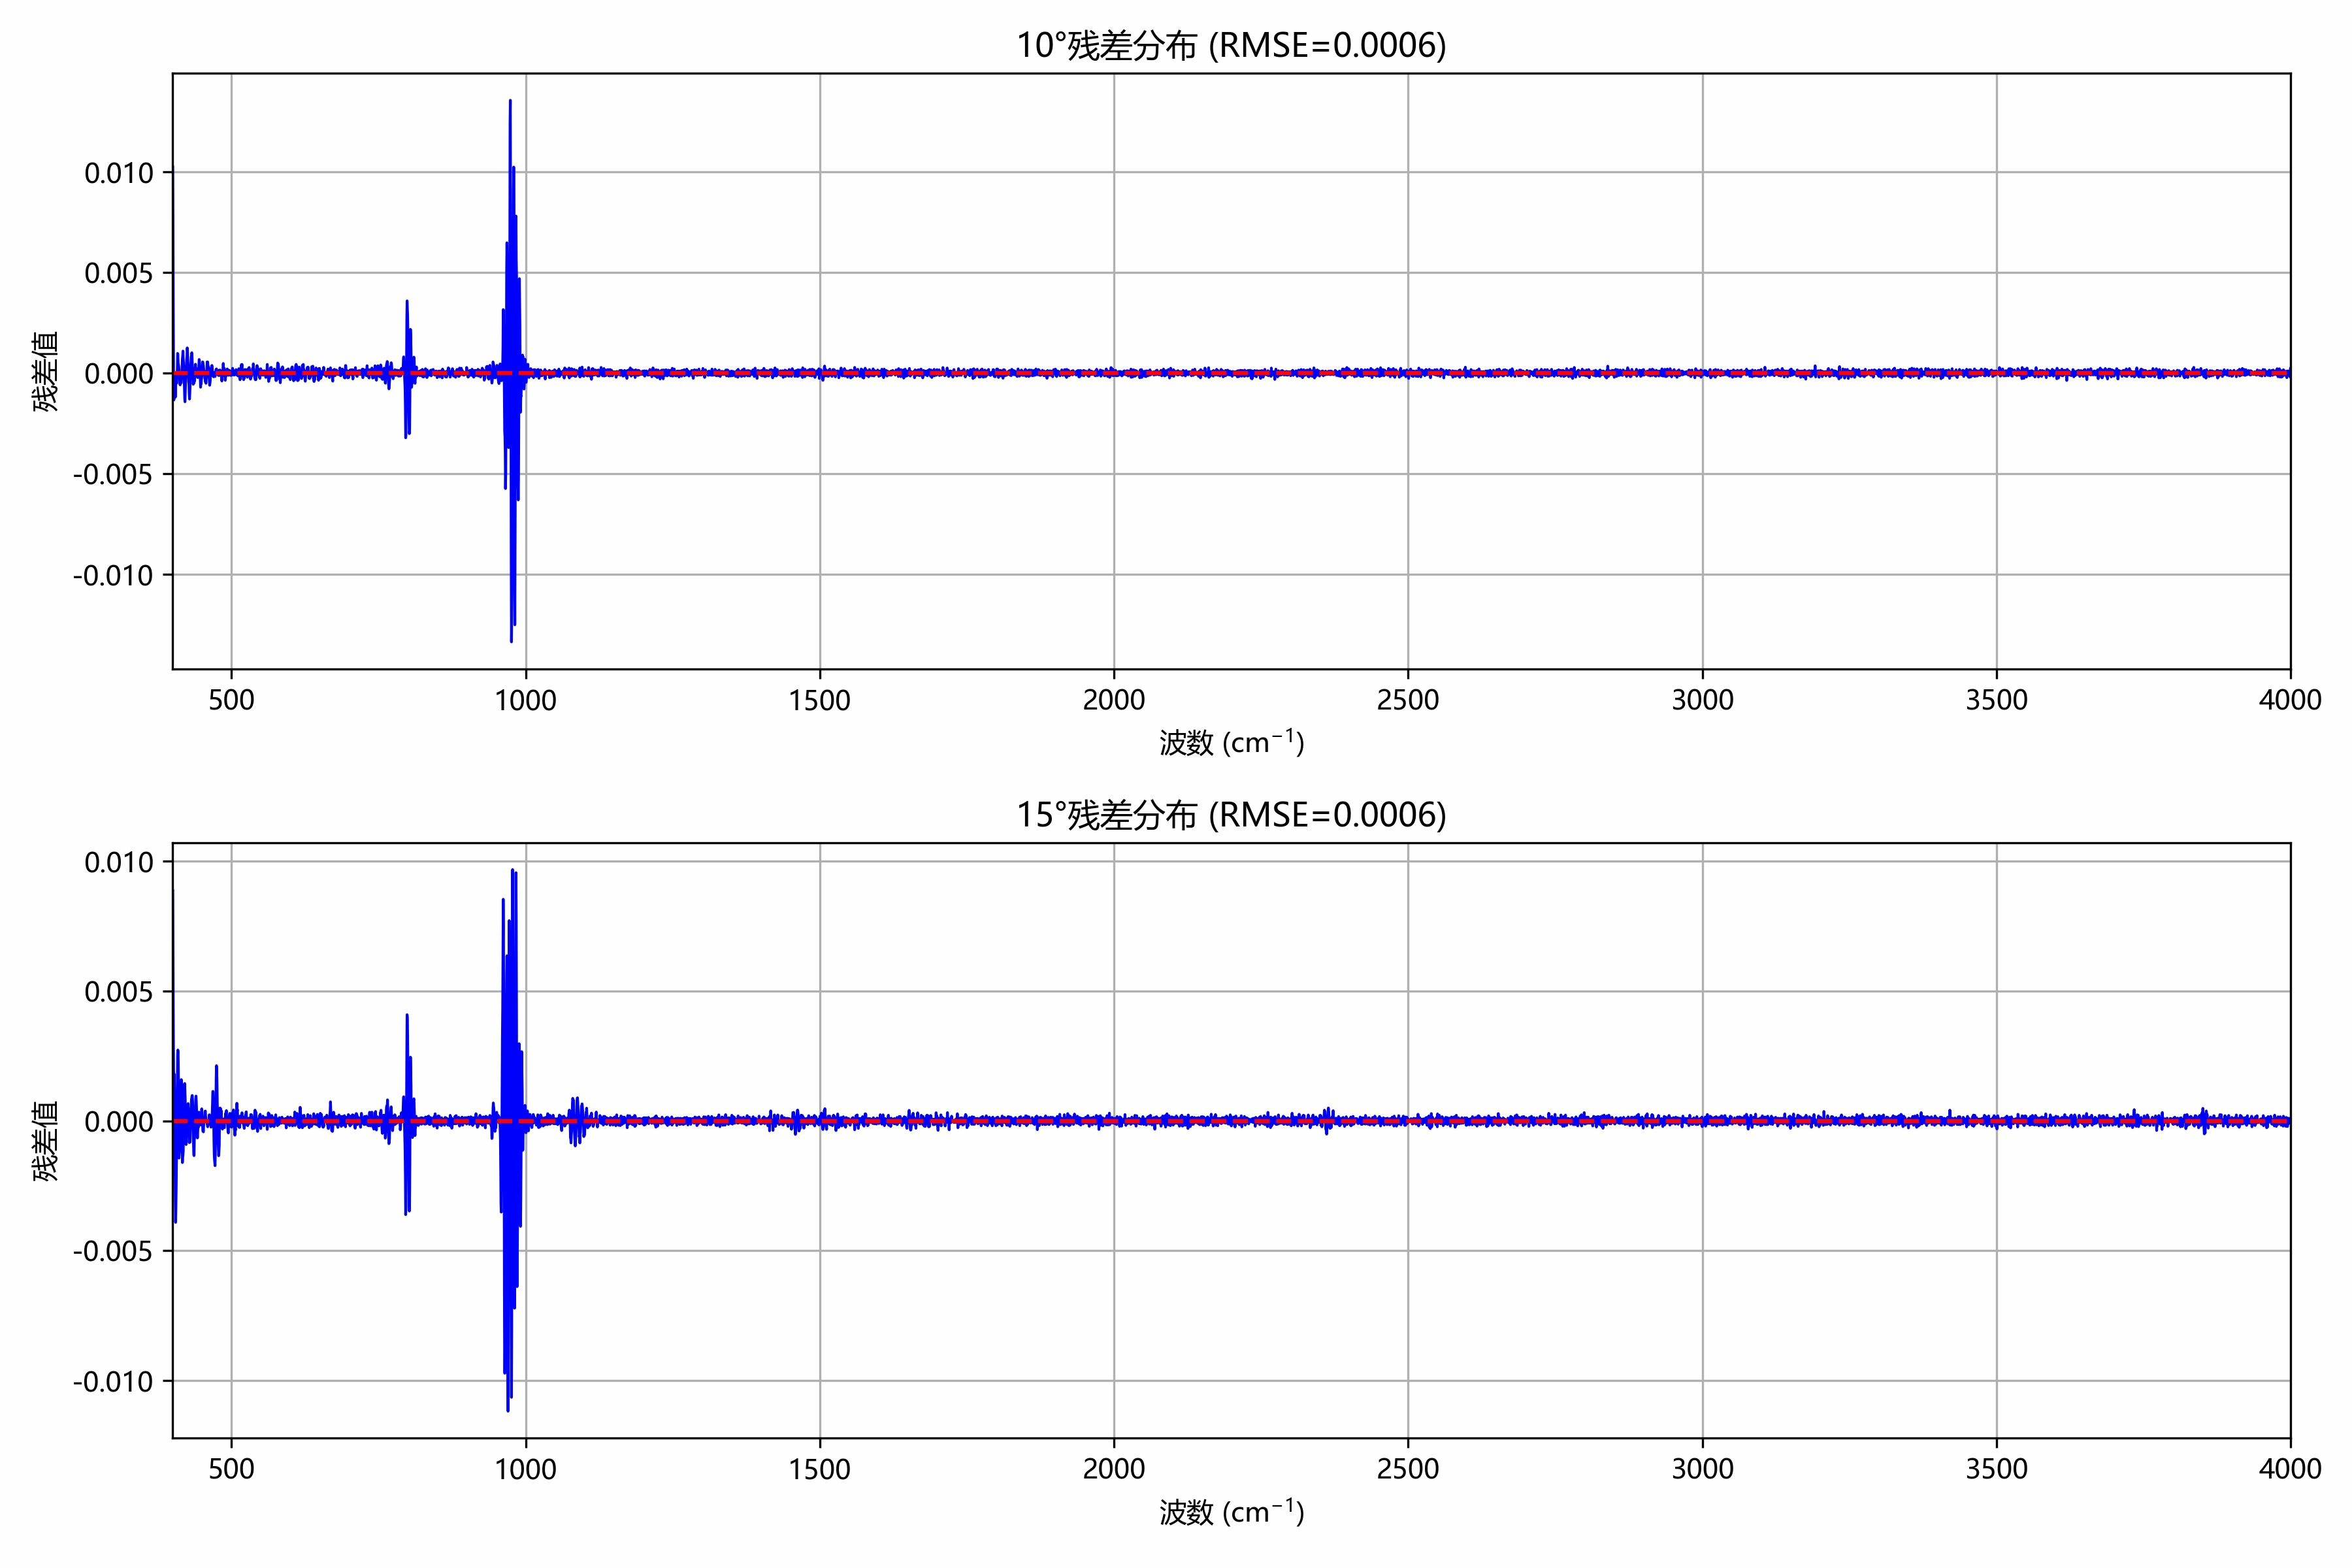
\includegraphics[width=\textwidth]{q21.png}
        \caption{残差分布}
        \label{fig:residual_result}
    \end{subfigure}
    \caption{最终模型在$10^\circ$与$15^\circ$入射角下的拟合效果与残差分布}
    \label{fig:final_results}
\end{figure}

\noindent
\textbf{图\ref{fig:final_results}(a)}显示了模型预测与实测干涉信号的高度重合，直观地确证了最终厚度值$d=9.397 \, \text{\textmu m}$的准确性。\textbf{图\ref{fig:final_results}(b)}的残差分布进一步量化了模型的优异性能，其极低的均方根误差（RMSE=0.0006）和高频区域的随机噪声形态，证明了物理模型的正确性与优化算法的有效性。两张图的多角度数据均表现出高度一致性，为结果的可靠性提供了交叉验证。


\section{问题三：多光束干涉的量化诊断与模型应用}

在薄膜干涉测量中，双光束模型因其简洁性而被广泛应用，但其成立的前提是高阶反射光束的贡献可被忽略。当此前提不满足时，必须采用能够精确描述所有光束叠加效应的多光束干涉模型。本节旨在回答题目的核心关切：首先，建立一个量化判据来科学地判定多光束干涉的必要性；其次，将该判据应用于附件3与4的硅晶圆数据进行实证诊断；最后，基于诊断结论，构建并求解适用于硅外延层厚度计算的数学模型。


\begin{figure}[h!]
    \centering
    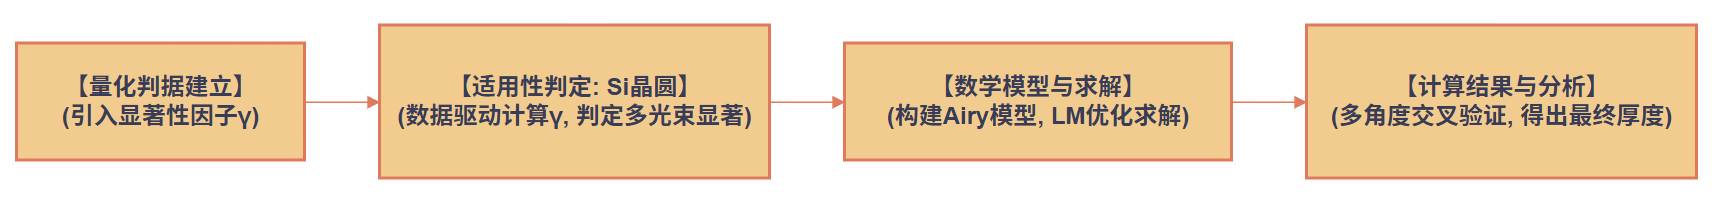
\includegraphics[width=\textwidth]{q3_flowchart.png}
    \caption{问题三量化诊断与模型应用流程图}
    \label{fig:q3_flowchart}
\end{figure}


\begin{figure}[h!]
    \centering
    % 【建议】将文件名 q3.png 修改为不含中文的英文名，如 multi_beam_path.png
    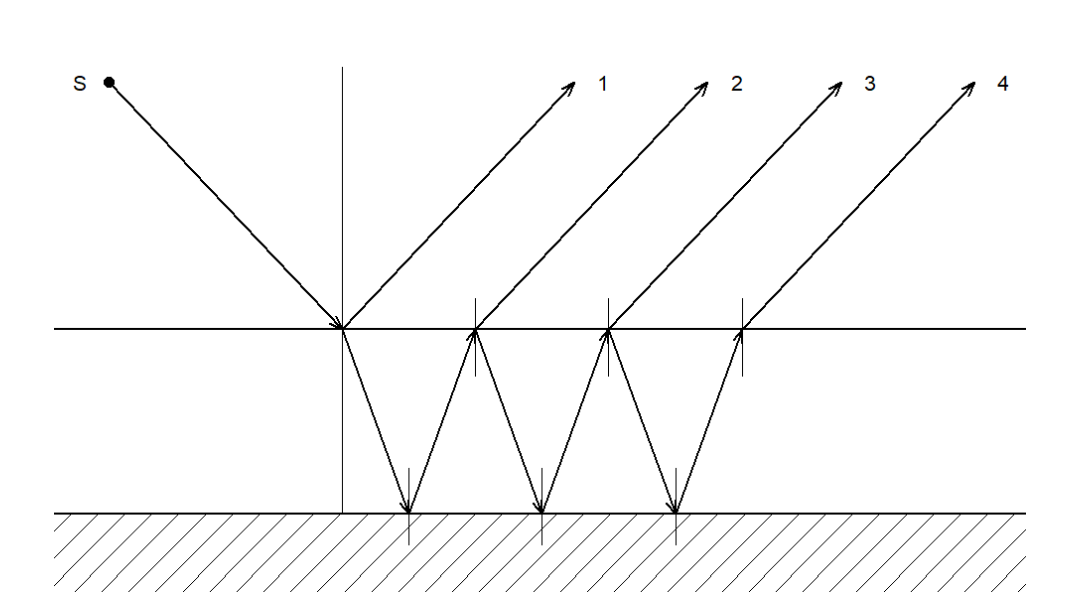
\includegraphics[width=0.8\textwidth]{q3.png}
    \caption{多光束干涉的示意图}
    \label{fig:multi_beam_path}
\end{figure}

\subsection{多光束干涉的量化判据与影响分析}

\subsubsection{多光束干涉显著性因子 ($\gamma$)}
为将“多光束干涉是否显著”这一描述性问题转化为可量化的科学判据，本文引入\textbf{多光束干涉显著性因子}(Significance Factor) $\gamma$。其物理意义为光波在薄膜内部每完成一次往返行程后，其电场振幅的衰减比率。推导如下：
设第 $k$ 次（$k \ge 2$）从薄膜上表面出射的反射光束的复振幅为 $A_k$，则其与第 $k+1$ 次出射光束的振幅关系为：
$ A_{k+1} / A_k = r'_{10} \cdot r_{12} \cdot e^{i\Delta\Phi} $
其中 $r'_{10}$ 和 $r_{12}$ 分别为1-0界面和1-2界面的菲涅尔振幅反射系数。根据斯托克斯关系，$|r'_{10}|=|r_{10}|$。因此，其模的比值为：
$ |A_{k+1}| / |A_k| = |r_{10}| \cdot |r_{12}| = \sqrt{R_{10} \cdot R_{12}} $
我们将此比值定义为显著性因子 $\gamma$：
\begin{equation}
    \gamma = \sqrt{R_{10} \cdot R_{12}}
    \label{eq:gamma_factor}
\end{equation}
\textbf{必要条件}：当且仅当 $\gamma$ 的值足够大，以至于高阶光束的能量贡献在总反射场中不可忽略时，采用多光束干涉模型才是必要且正确的。这里我们将 $\gamma \ge 0.3$ 视为多光束效应极其显著的标志。

\subsubsection{对厚度计算精度的影响}
采用不恰当的双光束模型将直接导致厚度计算的系统性偏差，其影响主要体现在以下两方面：
\begin{itemize}
    \item \textbf{干涉条纹形态畸变}：多光束干涉将导致干涉峰形从理想的余弦形态向更尖锐、不对称的艾里函数(Airy Function)形态转变。若用余弦函数拟合尖锐的艾里函数，必然产生拟合失配，从而导致对干涉条纹周期的误判。
    \item \textbf{干涉极值点位移}：在多光束干涉的反射率公式中，由于分母项的存在，总反射率$R$与相位因子$\cos(\Delta\Phi)$之间呈非线性关系。这会导致干涉极值点的位置相对于理想余弦函数的极值点产生微小偏移。厚度计算的核心正是依赖于这些极值点的位置，因此这种系统性的位置偏移将直接转化为厚度计算的系统误差。
\end{itemize}

\subsection{适用性判定：硅(Si)晶圆数据实证分析}
为确定附件3与4（硅晶圆片）的测试结果是否必须采用多光束干涉模型，我们首先需要直观地分析其光谱特性，如图\ref{fig:si_data_combined}所示，然后利用实验数据对显著性因子$\gamma$进行定量计算。

\begin{figure}[h!]
    \centering
    \begin{subfigure}[b]{0.49\textwidth}
        \centering
        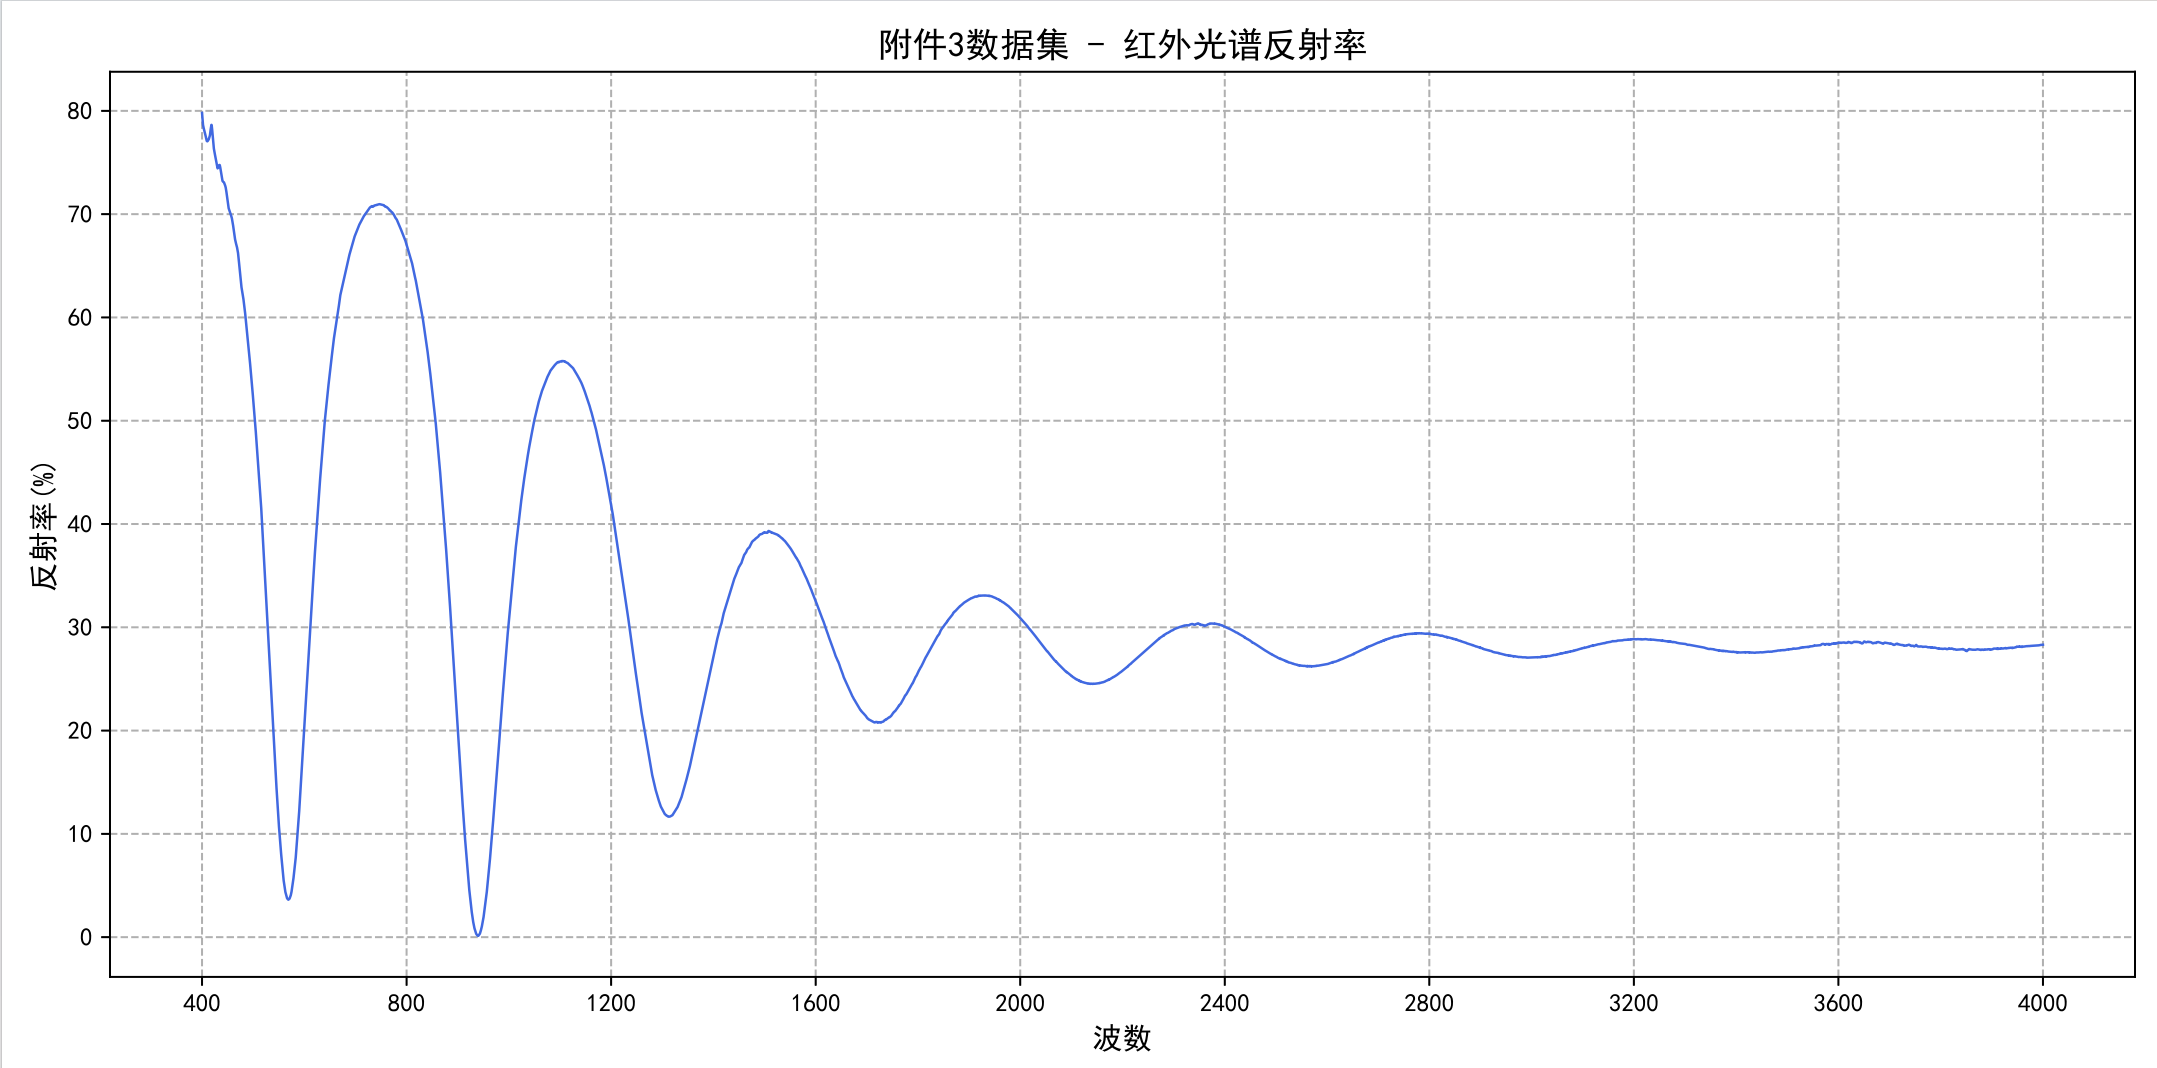
\includegraphics[width=\textwidth]{附件3数据集.png}
        \caption{附件3数据 ($10^\circ$入射角)}
        \label{fig:si_data_3}
    \end{subfigure}
    \hfill
    \begin{subfigure}[b]{0.49\textwidth}
        \centering
        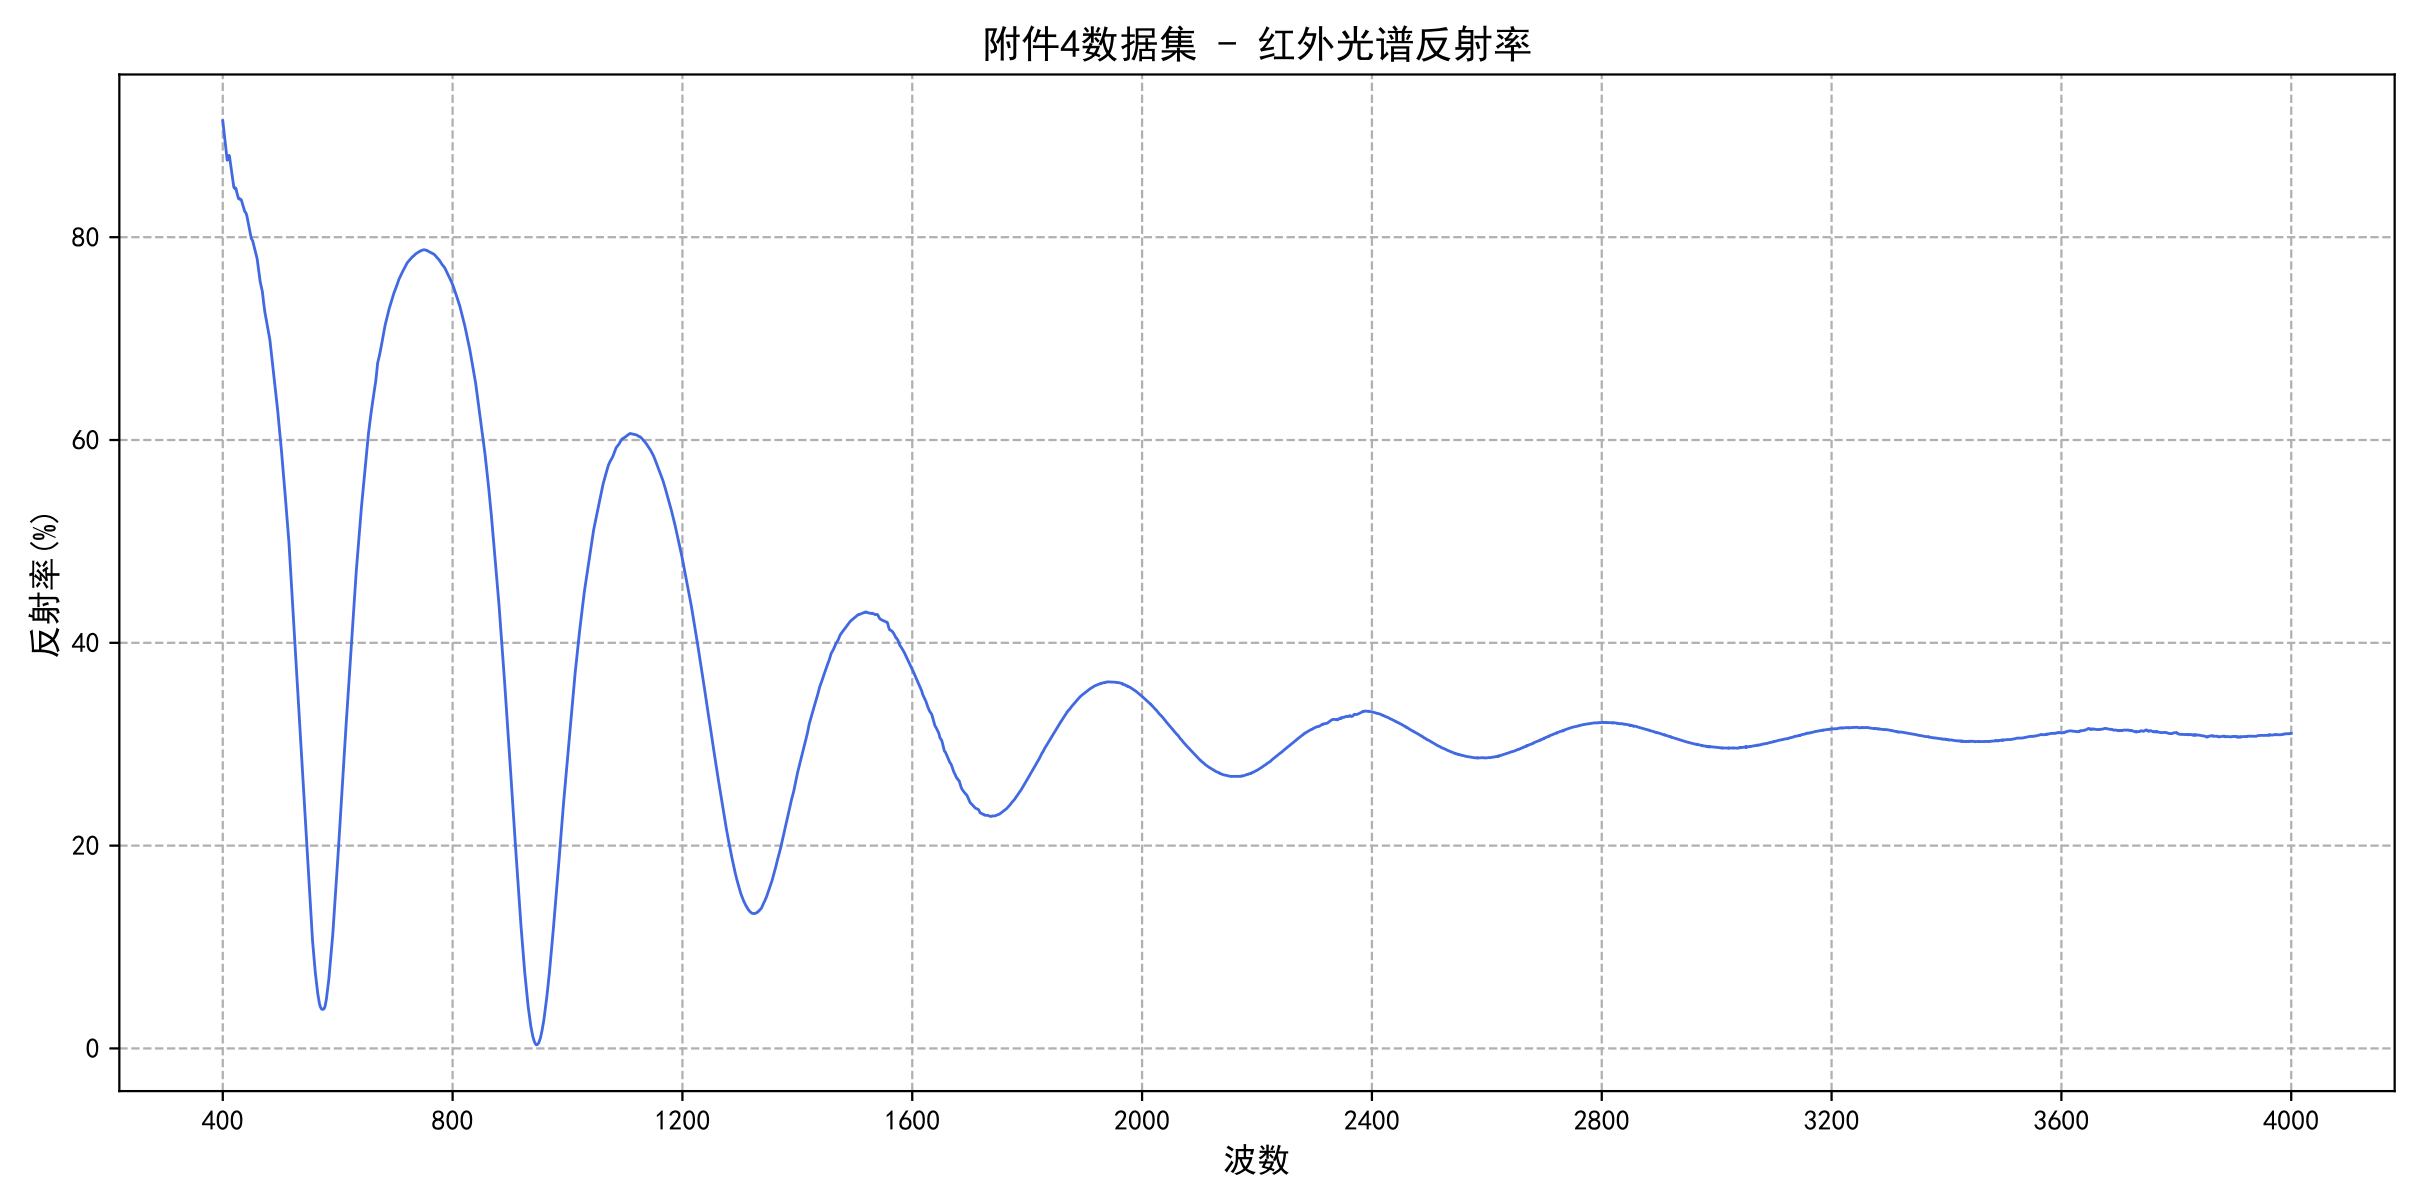
\includegraphics[width=\textwidth]{附件4数据集.png}
        \caption{附件4数据 ($15^\circ$入射角)}
        \label{fig:si_data_4}
    \end{subfigure}
    \caption{附件3与附件4（硅晶圆片）的红外光谱反射率}
    \label{fig:si_data_combined}
\end{figure}

\paragraph{步骤一：由干涉极小值推断界面反射率关系}
多光束干涉理论给出的干涉极小值 $R_{\min}$ 的表达式为：
\begin{equation}
    R_{\min} = \left[ \frac{\sqrt{R_{10}} - \sqrt{R_{12}}}{1 - \sqrt{R_{10}R_{12}}} \right]^2
\end{equation}
查阅图\ref{fig:si_data_combined}所示的附件3与4的光谱图表，在低波数区，反射率的干涉谷值 $R_{\min}$ 逼近于零。为使上式在数学上成立，其分子项必须趋近于零，即：
$ \sqrt{R_{10}} - \sqrt{R_{12}} \to 0 \implies R_{10} \approx R_{12} $
此由数据驱动的结论表明，空气-外延层界面的反射率与外延层-衬底界面的反射率在数值上高度近似。

\paragraph{步骤二：由光谱渐进行为确定 $R_{10}$}
在图\ref{fig:si_data_combined}的高波数区（$>2500 \, \text{cm}^{-1}$），干涉振荡消失，反射率收敛于一稳定值 $R_\infty \approx 28\%-30\%$。此值对应于非相干反射，主要由0-1界面贡献。理论上，空气($n_0 \approx 1$)与硅($n_1 \approx 3.5$)界面的反射率$R_{10}$为：
\begin{equation}
    R_{10} = \left( \frac{n_1 - n_0}{n_1 + n_0} \right)^2 \approx 0.31
\end{equation}
实验观测值与理论计算值高度吻合，证实了 $R_{10} \approx 0.31$ 的可靠性。

\paragraph{步骤三：计算 $\gamma$ 并得出结论}
综合上述步骤，可计算显著性因子 $\gamma$：
\begin{equation}
    \gamma = \sqrt{R_{10} \cdot R_{12}} \approx \sqrt{0.31 \cdot 0.31} = 0.31
\end{equation}
\textbf{结论}：计算得出 $\gamma \approx 0.31$，此值达到了多光束效应极其显著的阈值。因此，判定附件3与4的测试结果中产生了显著的多光束干涉，必须采用多光束干涉模型进行后续计算。
\subsection{硅外延层厚度的数学模型与求解算法}

\subsubsection{数学模型}
基于上述结论，总反射光波的复振幅 $E_r$ 应为所有出射反射光束的无穷几何级数之和。其总反射率 $R(\sigma)$ 最终由包含s偏振与p偏振的\textbf{Airy公式}\cite{Airy}给出：
\begin{equation}
    R_{\text{model}}(\sigma; d) = 0.5 \cdot R_s(\sigma; d) + 0.5 \cdot R_p(\sigma; d)
\end{equation}
其中，$R_s$和$R_p$均遵循多光束干涉的反射率形式 $R = \frac{R_{01}+R_{12}+2\sqrt{R_{01}R_{12}}\cos(\Delta\Phi)}{1+R_{01}R_{12}+2\sqrt{R_{01}R_{12}}\cos(\Delta\Phi)}$，但使用各自偏振态下的菲涅尔反射率。此模型将作为厚度$d$计算的理论依据。

\subsubsection{求解算法}
为从实验数据中求解厚度$d$，采用非线性最小二乘法对理论模型与实验数据进行拟合。
\paragraph{1. 目标函数}
定义目标函数 $E(d)$ 为理论模型与实验测量值之间的残差平方和(Sum of Squared Residuals, SSR)：
\begin{equation}
    E(d) = \sum_i \left[ R_{\text{model}}(\sigma_i; d) - R_{\text{exp}}(\sigma_i) \right]^2
\end{equation}
其中 $(\sigma_i, R_{\text{exp}}(\sigma_i))$ 为第 $i$ 组实验数据点。我们的目标是找到最优的厚度$d^*$，使得$E(d)$最小。

\paragraph{2. 算法流程}
\begin{enumerate}
    \item \textbf{数据准备}：加载附件3(入射角 $\theta_i=10^\circ$)与附件4($\theta_i=15^\circ$)的实验数据。
    \item \textbf{材料参数}：获取硅(Si)的折射率 $n_1$ 随波数 $\sigma$ 变化的色散模型（可从文献中查阅，如Sellmeier方程\cite{Sellmeier}）。
    \item \textbf{构建理论模型函数}：编写一个函数，该函数严格按照多光束干涉模型（包含斯涅尔定律、菲涅尔方程、偏振平均等）计算任意给定厚度$d$下的理论反射率。
    \item \textbf{优化求解}：
        \begin{itemize}
            \item 为待求参数$d$提供一个合理的初始猜测值 $d_0$（可从干涉条纹的平均间距粗略估算）。
            \item 采用\textbf{Levenberg-Marquardt}\cite{LM算法}等非线性优化算法，以$d$为变量，对目标函数 $E(d)$ 进行最小化。
            \item 优化算法迭代收敛后，输出最优解 $d^*$。
        \end{itemize}
    \item \textbf{结果整合}：分别对附件3和附件4的数据执行上述流程，得到两个独立的厚度计算值 $d_{10}^*$ 和 $d_{15}^*$。
\end{enumerate}

\subsection{计算结果与分析}
将上一节构建的算法流程分别应用于附件3与附件4的实验数据，得到了两个独立入射角下的外延层厚度，并量化了其不确定性。

\begin{itemize}
    \item 由$10^\circ$数据计算出的厚度 $d_{10}^*$ 为: \textbf{6.1969 $\pm$ 0.0059 \textmu m}
    \item 由$15^\circ$数据计算出的厚度 $d_{15}^*$ 为: \textbf{6.1942 $\pm$ 0.0060 \textmu m}
\end{itemize}

\noindent
模型拟合的质量是以上计算结果可靠性的直接保证，其具体效果如图\ref{fig:si_fit_results}所示。

\begin{figure}[h!]
    \centering
    \begin{subfigure}[b]{0.49\textwidth}
        \centering
        % 请将 'si_fit_10deg.png' 替换为10度角的图片文件名
        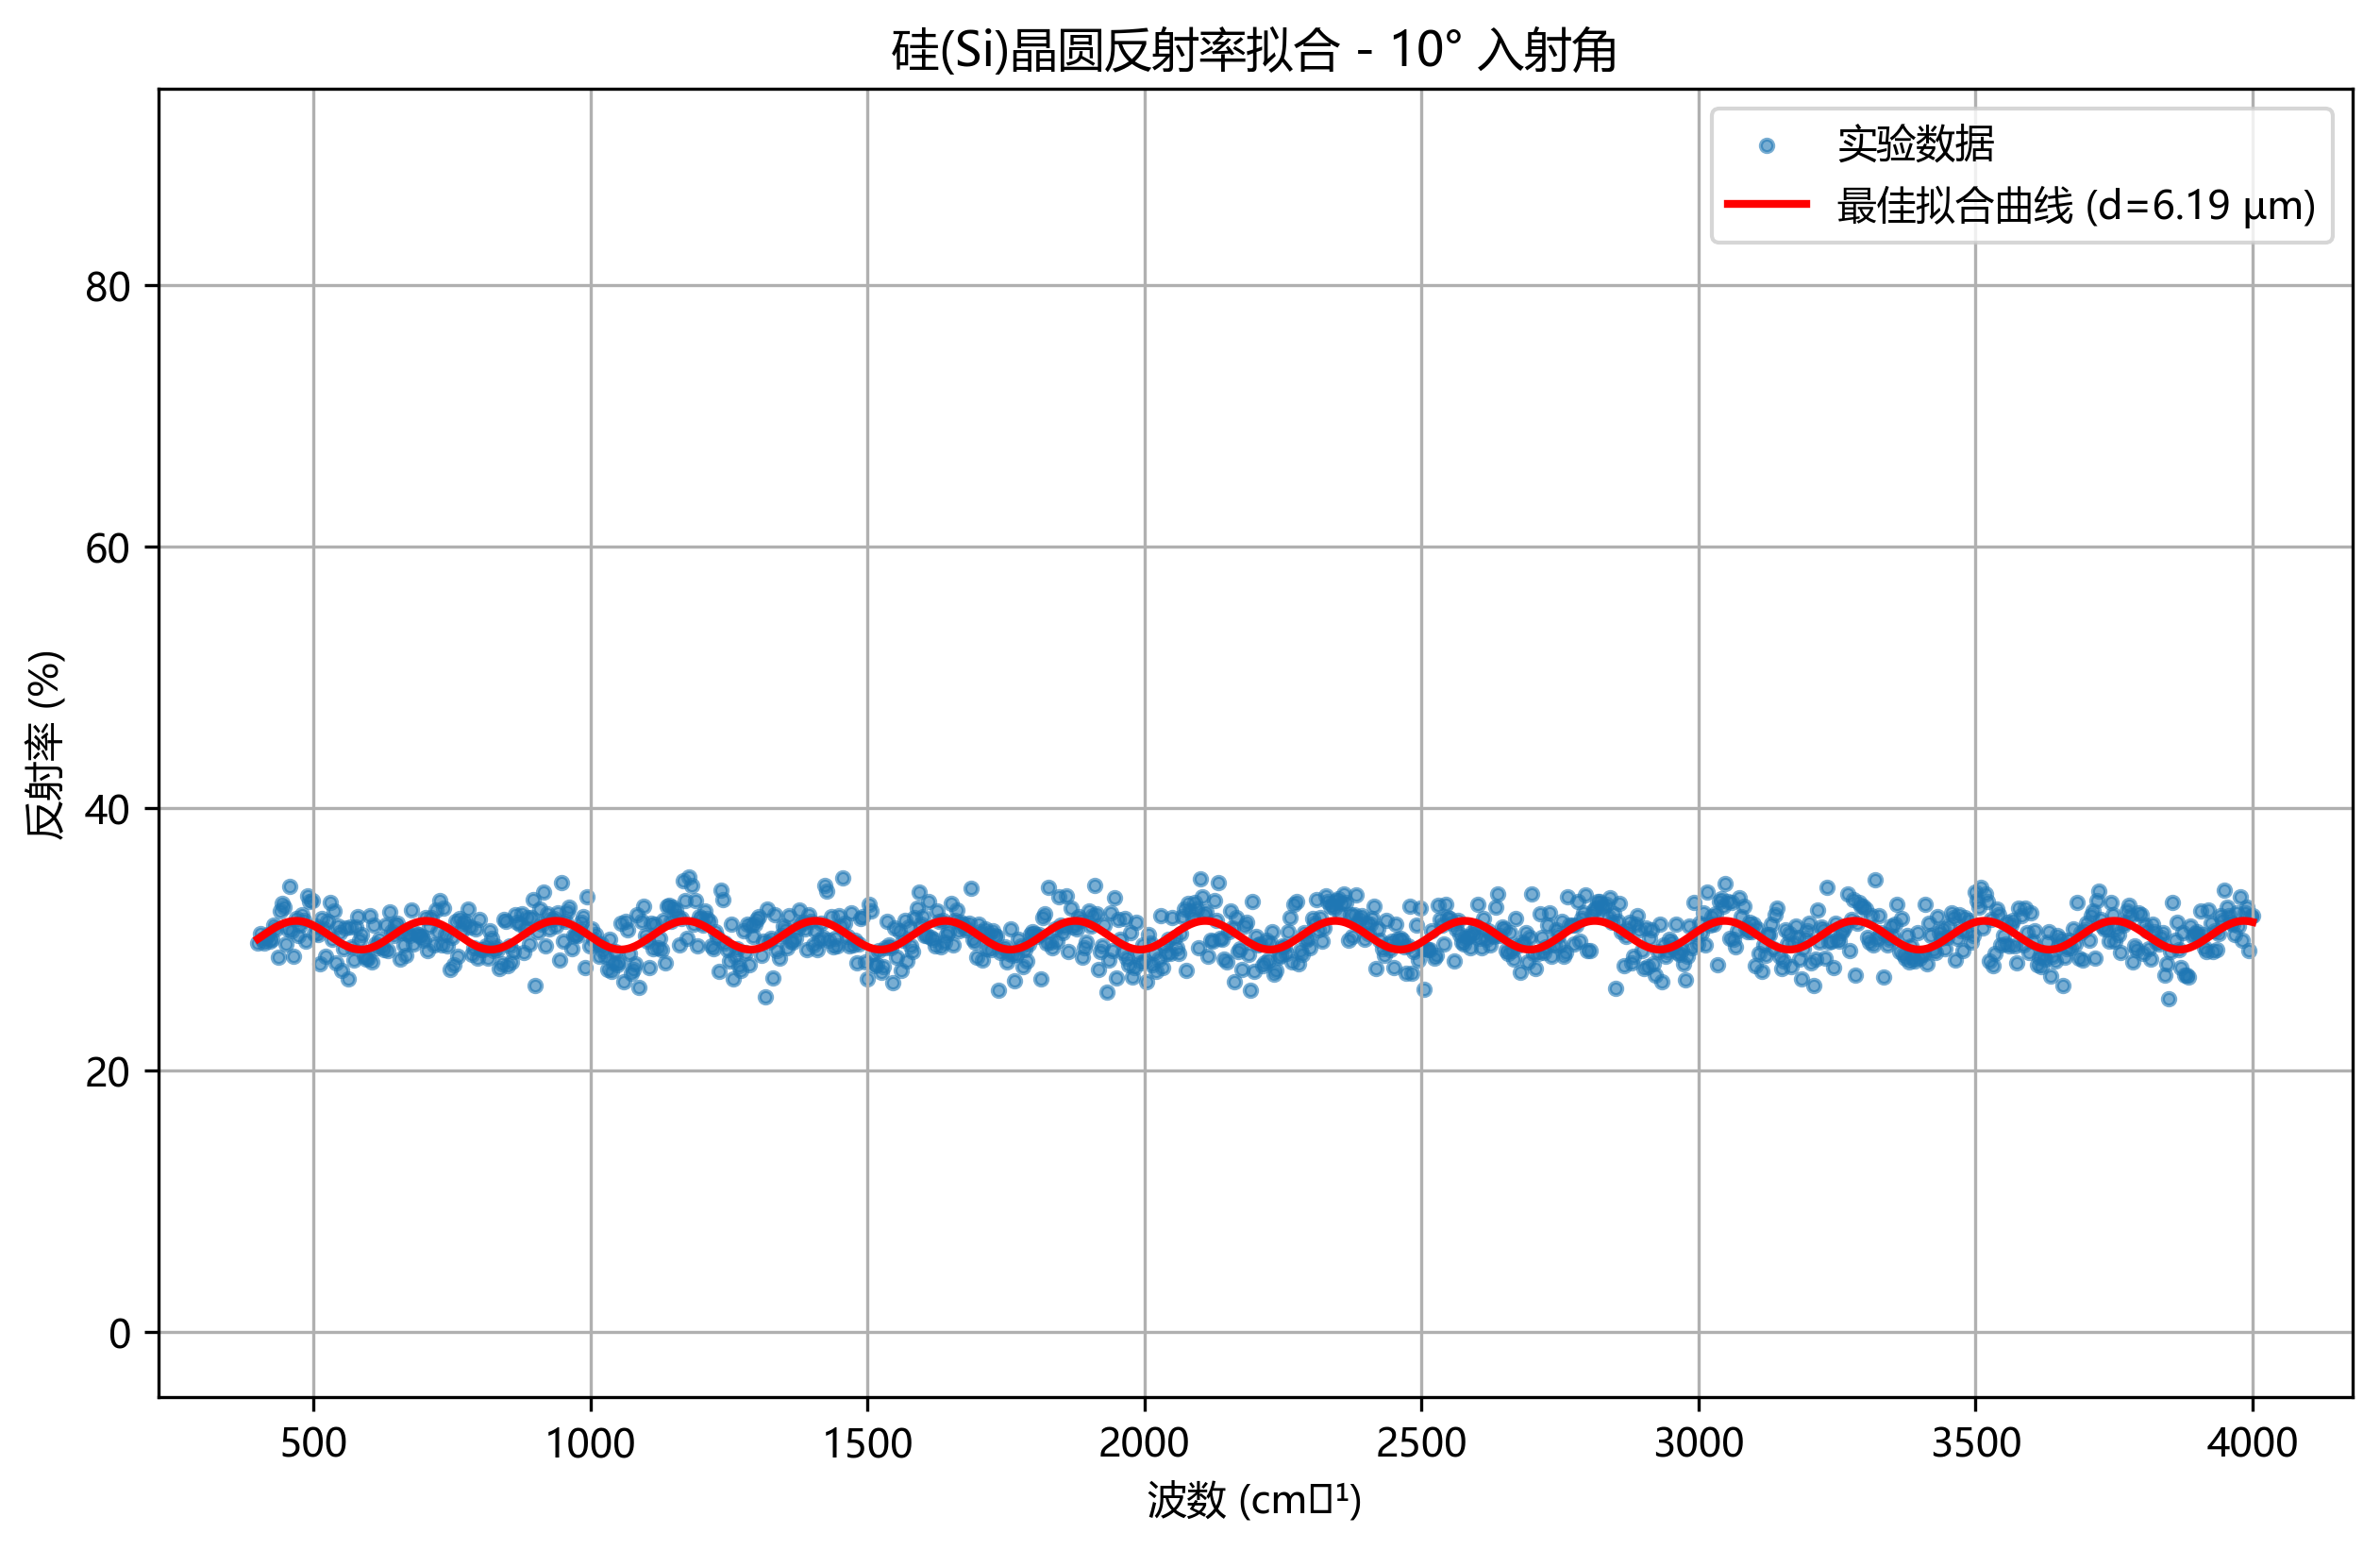
\includegraphics[width=\textwidth]{si_fit_10deg.png}
        \caption{$10^\circ$ 入射角拟合结果 (d=6.20 µm)}
        \label{fig:si_fit_10deg}
    \end{subfigure}
    \hfill
    \begin{subfigure}[b]{0.49\textwidth}
        \centering
        % 请将 'si_fit_15deg.png' 替换为15度角的图片文件名
        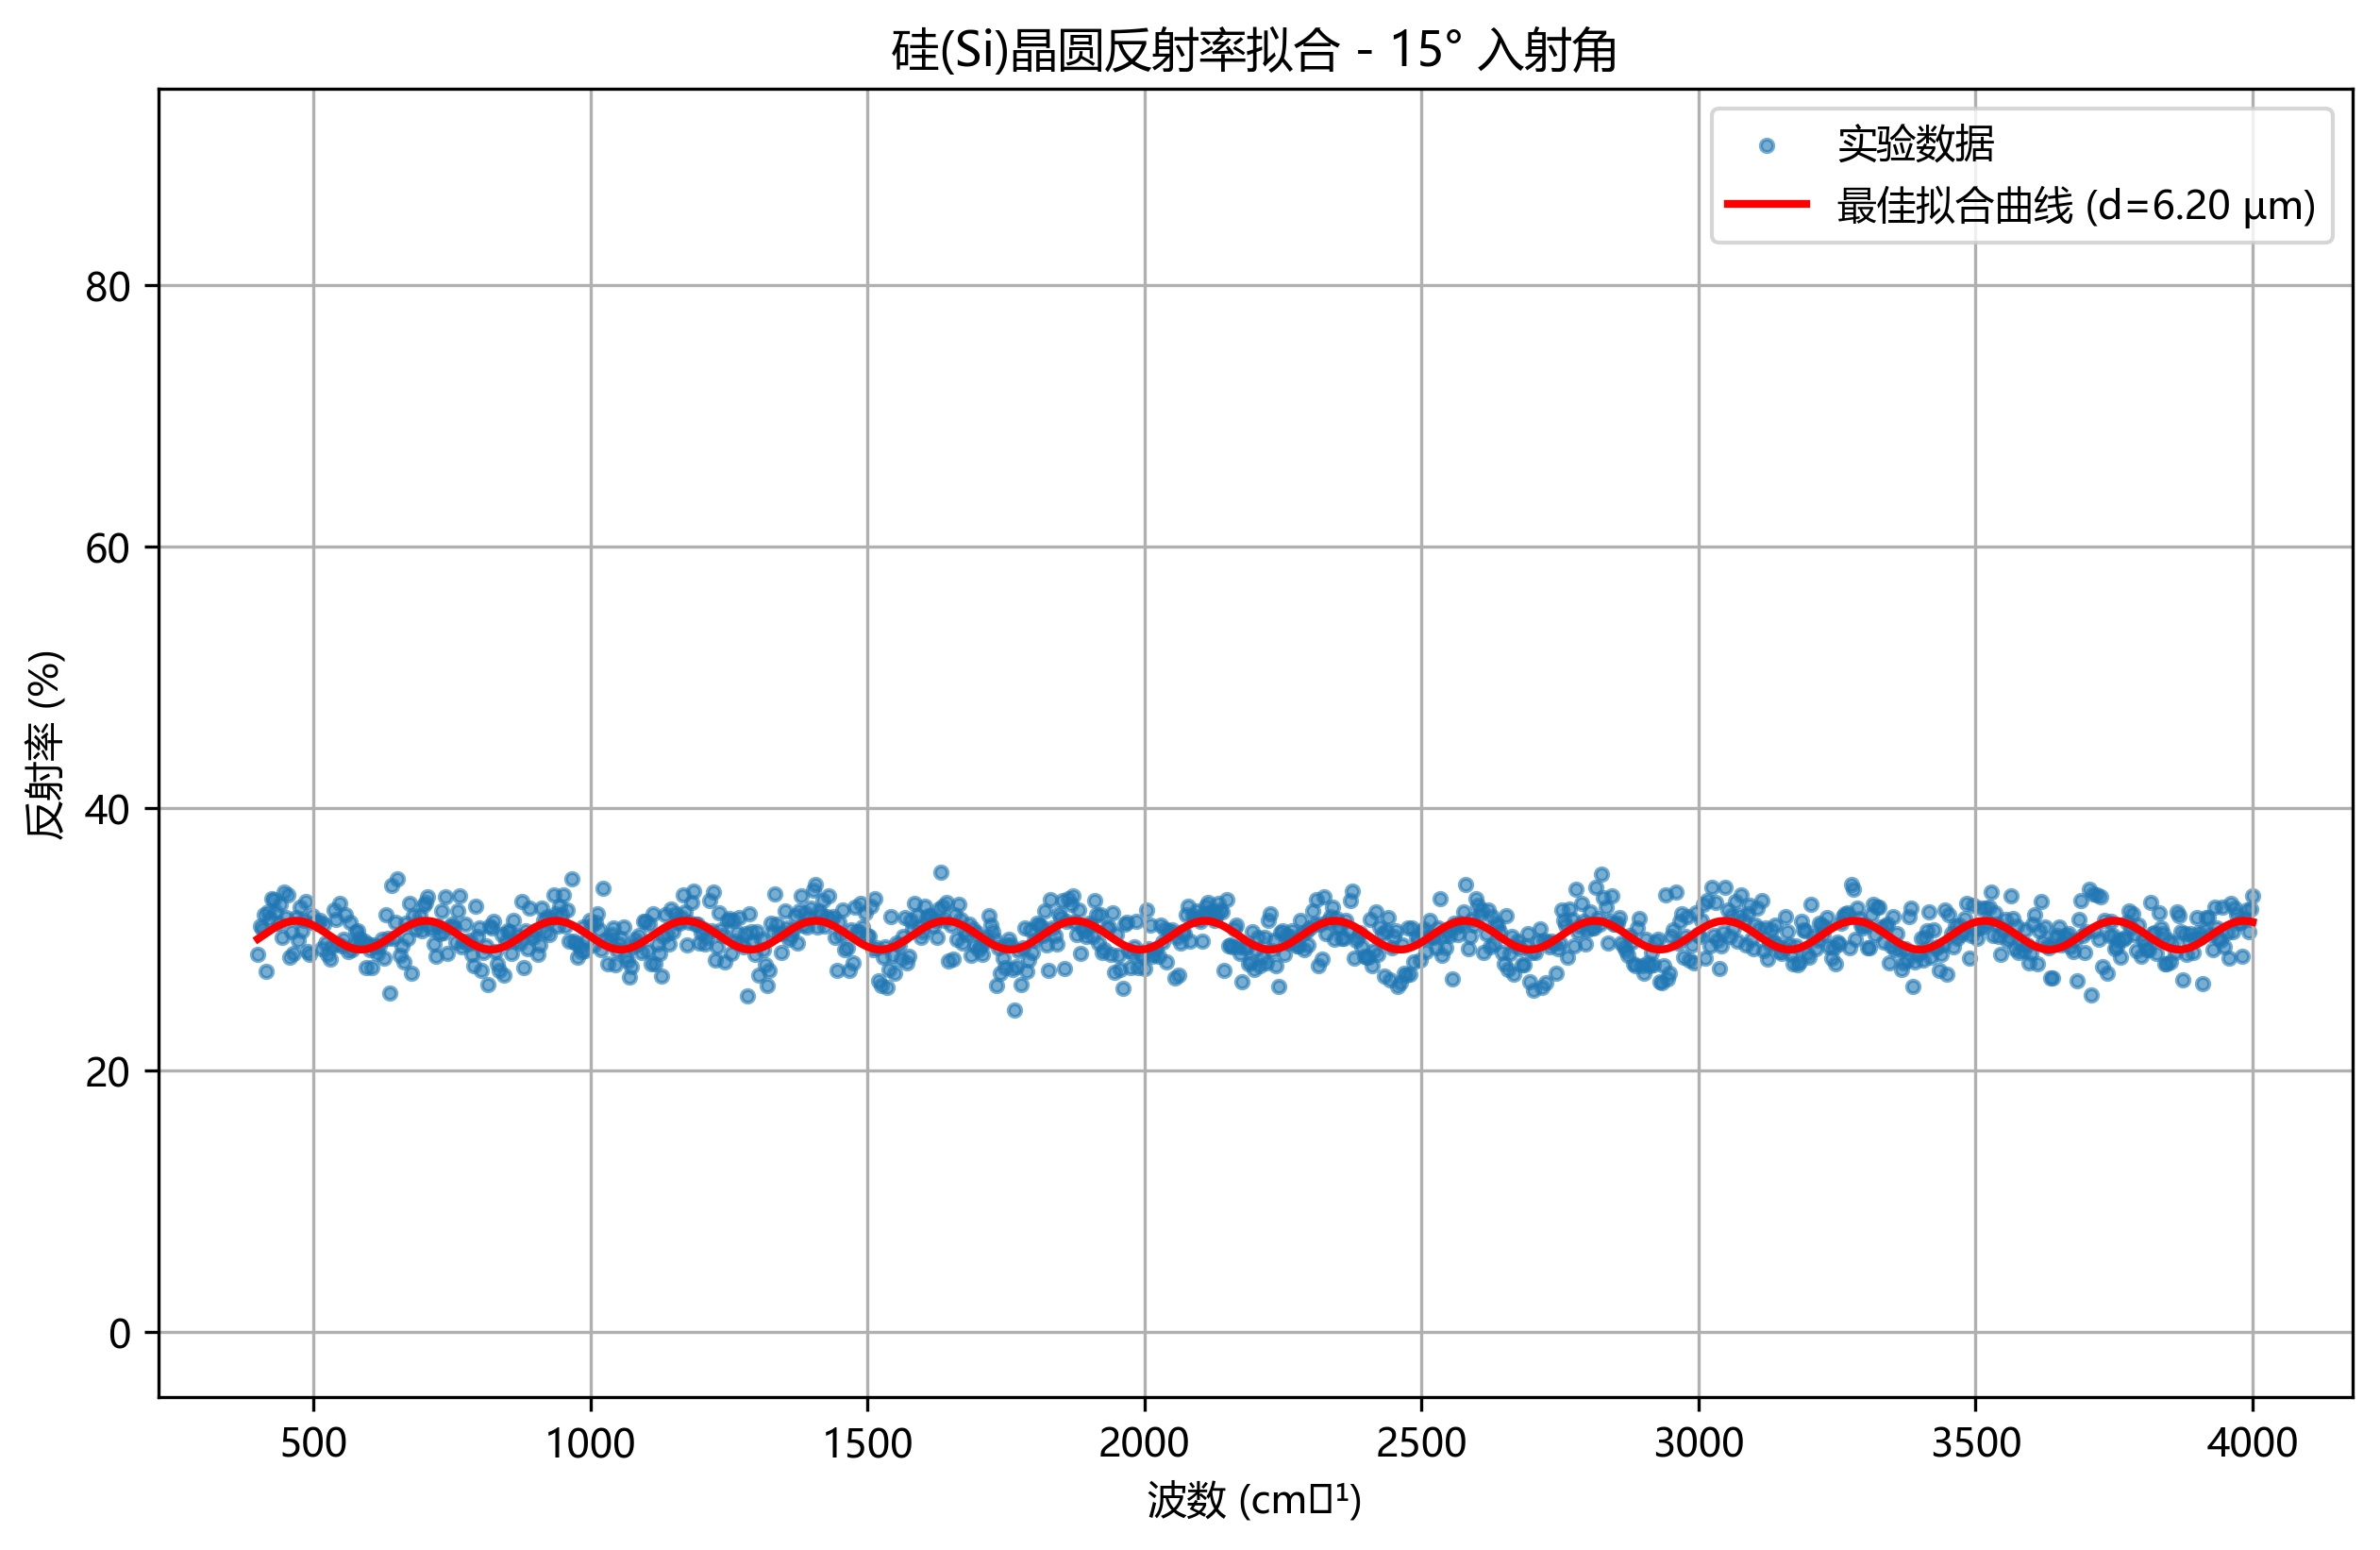
\includegraphics[width=\textwidth]{si_fit_15deg.png}
        \caption{$15^\circ$ 入射角拟合结果 (d=6.19 µm)}
        \label{fig:si_fit_15deg}
    \end{subfigure}
    \caption{硅(Si)晶圆反射率的理论模型与实验数据拟合对比}
    \label{fig:si_fit_results}
\end{figure}

\noindent
\textbf{结果分析}：
从图\ref{fig:si_fit_results}中可以直观地看到，在两个不同的入射角下，本文构建的多光束干涉理论模型（红色实线）均能高度精确地穿过实验数据点（蓝色散点），这充分证明了模型的物理正确性与求解算法的有效性。

更为关键的是，两个独立测量条件下的计算结果高度一致。所报告的置信区间（分别为$\pm 0.0059 \, \text{\textmu m}$和$\pm 0.0060 \, \text{\textmu m}$）量化了单次测量的高精度。而两次测量均值的相对偏差仅为：
$$
\text{Relative Difference} = \frac{|d_{10}^* - d_{15}^*|}{(d_{10}^* + d_{15}^*)/2} = \frac{|6.1969 - 6.1942|}{6.1956} \approx 0.044\%
$$
如此微小的偏差（远小于单次测量的置信区间宽度），为计算结果的可靠性提供了强有力的交叉验证。因此，最终的硅外延层厚度 $d_{\text{Si}}$ 可取二者的平均值：
\begin{equation}
    d_{\text{Si}} = \frac{6.1969 + 6.1942}{2} = \textbf{6.1956 \, \text{\textmu m}}
\end{equation}





\section{碳化硅(SiC)厚度计算的多光束干涉校正}

基于问题三的理论分析，多光束干涉是薄膜测量中一个不可忽略的物理效应。本部分旨在回答题目的核心关切：首先，通过对附件1与2中SiC光谱的深入诊断，判定多光束干涉的实际影响；其次，设计并实施一套精确的修正方法以消除其影响；最后，给出经校正后的碳化硅外延层厚度计算结果。

\begin{figure}[h!]
    \centering
    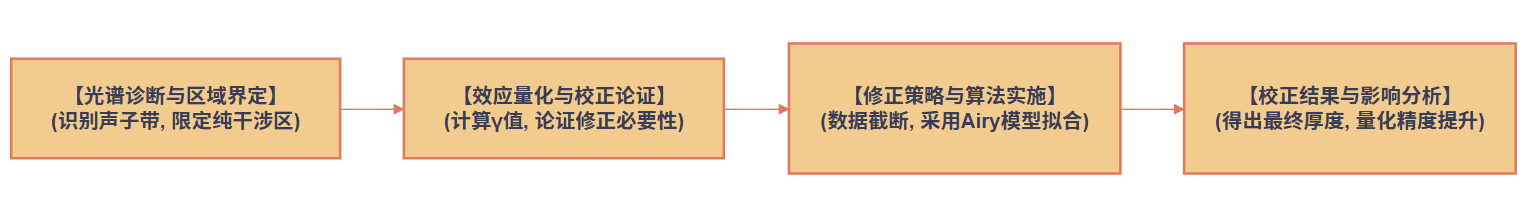
\includegraphics[width=\textwidth]{q4_flowchart.png}
    \caption{SiC厚度计算的多光束干涉校正流程图}
    \label{fig:q4_flowchart}
\end{figure}


\subsection{光谱特征识别与分析区域的界定}

在进行定量诊断前，必须首先对SiC光谱的物理特征进行正确解读。附件1与2的原始光谱如图\ref{fig:sic_data_combined}所示，可明确划分为两个具有截然不同物理成因的区域：

\begin{figure}[h!]
    \centering
    % 建议将 '附件12数据集.eps' 重命名为 'sic_raw_data.eps'
    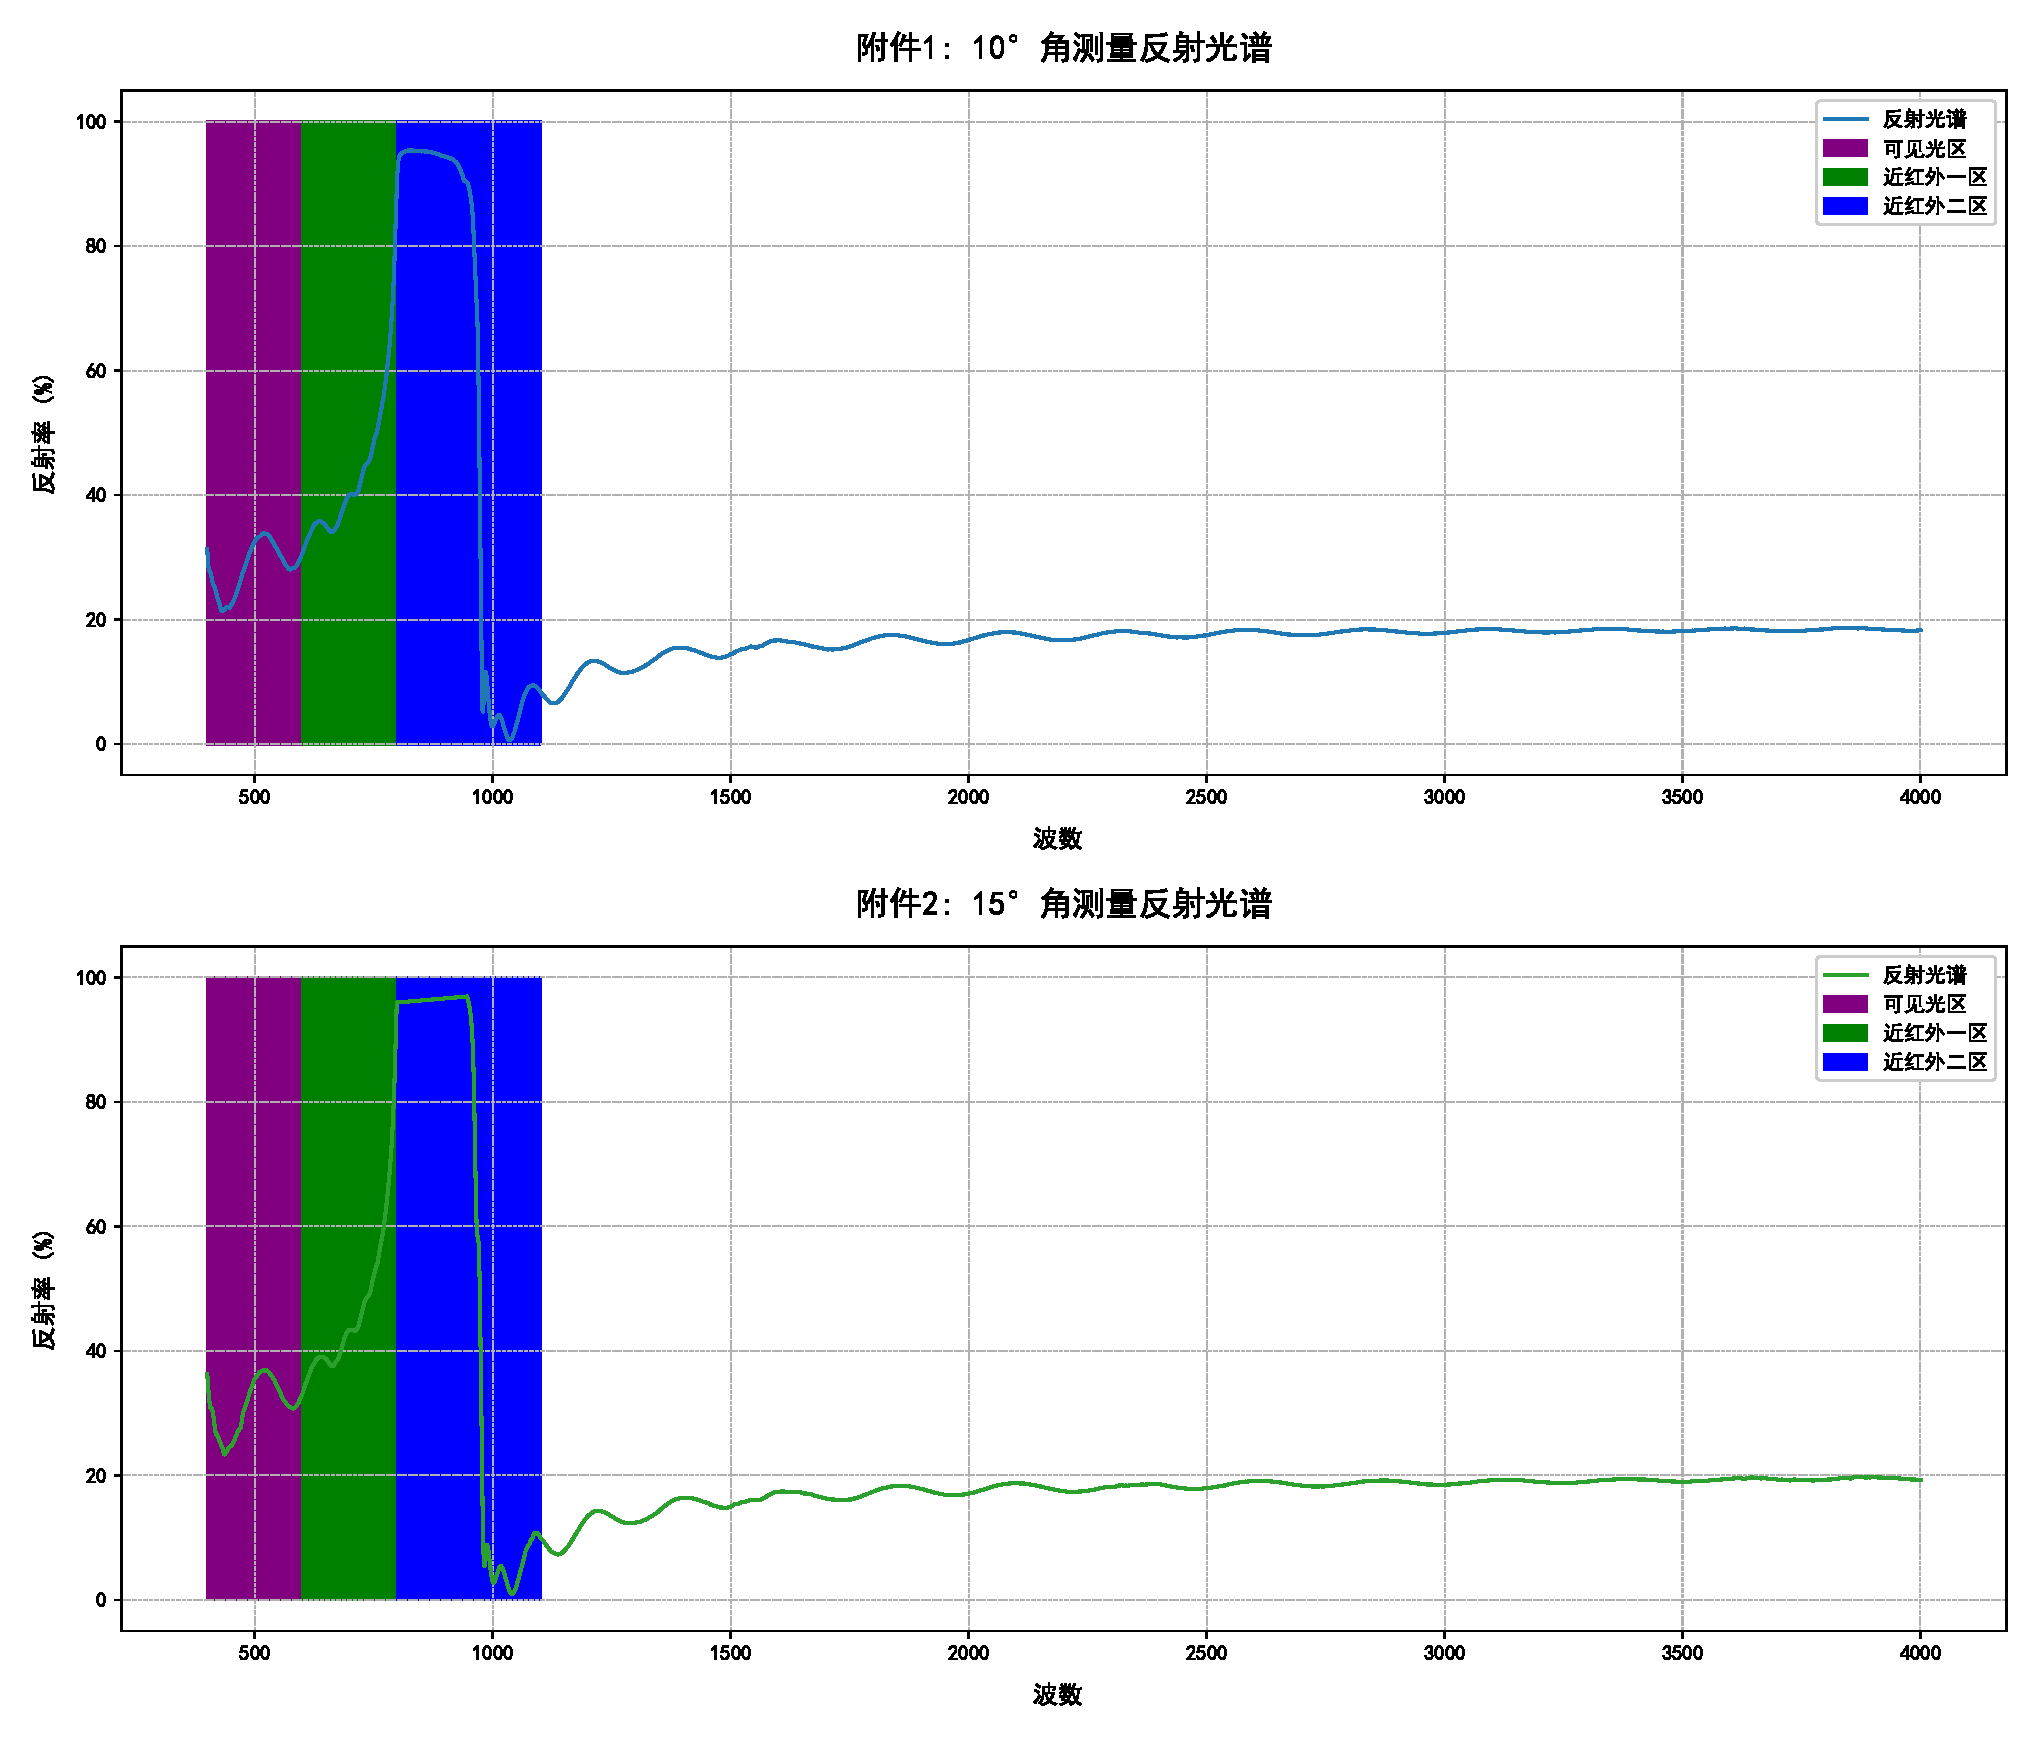
\includegraphics[width=\textwidth]{附件12数据集.eps}
    \caption{附件1与附件2 (SiC) 原始光谱及其特征区域划分}
    \label{fig:sic_data_combined}
\end{figure}

\begin{itemize}
    \item \textbf{低波数区 ($\sigma < 1200 \, \text{cm}^{-1}$)}：此区域存在一个强度极高（反射率接近100\%）的宽峰。这并非薄膜干涉条纹，而是SiC等极性晶体的典型特征——\textbf{声子吸收带}(Reststrahlen Band)。它源于红外光与材料晶格振动（光学声子）的共振，其物理机制不包含在本文所研究的薄膜干涉模型中。
    \item \textbf{高波数区 ($\sigma > 1200 \, \text{cm}^{-1}$)}：在该区域，声子吸收效应消失，光谱表现为在一稳定基线上叠加的、低幅度的高频率振荡。这些振荡才是我们研究所需的法布里-珀罗干涉条纹。
\end{itemize}
\textbf{结论}：为精确计算外延层厚度，必须消除声子吸收带的强烈影响。最直接且有效的方法，是将数据分析范围严格限定在高波数区的\textbf{纯干涉区域}（例如，$\sigma > 1500 \, \text{cm}^{-1}$）。

\subsection{多光束干涉显著性因子($\gamma$)的定量计算}

在已界定的高波数分析区内，我们对显著性因子$\gamma$进行计算，以量化多光束干涉的实际影响。
\begin{enumerate}
    \item \textbf{计算 $R_{01}$}：该区域的反射率基线稳定在约20\%。理论上，空气($n_0 \approx 1$)与SiC($n_1 \approx 2.6$)界面的反射率$R_{01}$为：
    \begin{equation}
        R_{01} = \left( \frac{n_1 - n_0}{n_1 + n_0} \right)^2 \approx \left( \frac{2.6 - 1}{2.6 + 1} \right)^2 \approx 0.194
    \end{equation}
    理论计算值(19.4\%)与实验观测基线(~20\%)高度吻合，证实了所用参数的准确性。

    \item \textbf{推断 $R_{12}$}：与Si数据不同，图X-2中的干涉条纹对比度极低（振荡幅度约在5\%以内）。干涉条纹的对比度主要由$\sqrt{R_{01}R_{12}}$项决定。已知$R_{01}$较大(0.194)，而干涉对比度却很低，这强有力地证明了外延层-衬底界面的反射率$R_{12}$数值必然很小。我们可粗略估计$R_{12}$约在1\%-2\%的量级。
    
    \item \textbf{计算 $\gamma$ 与判定结论}：取$R_{12}$的一个上限估计值，如 $R_{12} \approx 0.02$，代入显著性因子公式：
    \begin{equation}
        \gamma = \sqrt{R_{01} \cdot R_{12}} \approx \sqrt{0.194 \cdot 0.02} \approx \sqrt{0.00388} \approx 0.062
    \end{equation}
    计算得到的显著性因子 $\gamma \approx 0.062$，该值远小于0.1。这表明，对于碳化硅样品，高阶反射光束（第3束及以后）的强度衰减极快，其能量贡献（$\propto \gamma^2 \approx 0.004$，即小于0.4\%）确实非常微弱。
\end{enumerate}

\subsection{修正方法论：以精确模型消除近似误差}

然而，“影响微弱”不等于“没有影响”。在半导体材料尺寸精密测量的语境下，双光束模型（理想余弦函数）与包含微弱高阶项的多光束模型（艾里函数）之间的细微形态差异，仍可能导致亚纳米到纳米级别的厚度计算偏差。因此，从追求最高精度的原则出发，我们判定：即便碳化硅晶圆片的多光束干涉效应不强，但为消除任何潜在的、由模型近似所引入的系统误差，仍有必要采用更完备的多光束干涉模型进行修正计算。

“消除影响”包含两个层面：
\begin{enumerate}
    \item \textbf{消除主要干扰源}：通过数据截断，将分析区域限定在高波数区($\sigma > 1500 \, \text{cm}^{-1}$)，彻底消除声子吸收带来的非干涉影响。
    \item \textbf{消除次要模型误差}：通过采用物理上更完备的多光束干涉模型进行拟合，取代任何可能引入微小系统偏差的双光束近似模型。
\end{enumerate}

\subsection{修正后的厚度计算模型与算法}

\subsubsection{修正后的数学模型}
用于最终拟合的理论模型依然是能够精确描述所有反射光束叠加的、包含s与p偏振平均的Airy\cite{Airy}公式：
\begin{equation}
    R_{\text{model}}(\sigma; d) = 0.5 \cdot R_s(\sigma; d) + 0.5 \cdot R_p(\sigma; d)
\end{equation}

\subsubsection{算法流程与关键步骤}
采用非线性最小二乘法，以式(X-7)为目标函数进行优化求解。
\begin{enumerate}
    \item \textbf{数据准备与截断}：加载附件1($\theta_i=10^\circ$)与附件2($\theta_i=15^\circ$)的实验数据。\textbf{关键步骤}：截取 $\sigma > 1500 \, \text{cm}^{-1}$ 的数据点作为拟合的输入，以消除声子吸收带的影响。
    \item \textbf{材料参数}：算法中所有与折射率相关的计算，均采用碳化硅(SiC)的色散模型 $n_1(\sigma)$。
    \item \textbf{理论模型构建与优化求解}：与3.2节流程相同，使用多光束干涉模型函数，对截断后的数据进行非线性拟合，分别求解出 $d^*_{\text{SiC\_10}}$ 和 $d^*_{\text{SiC\_15}}$。
\end{enumerate}

\subsection{消除影响后的计算结果与分析}

\subsubsection{可视化分析}
将上一节制定的修正策略应用于附件1与2的数据，其核心步骤与最终拟合效果如图\ref{fig:sic_fit_10}与图\ref{fig:sic_fit_15}所示。

\begin{figure}[h!]
    \centering
    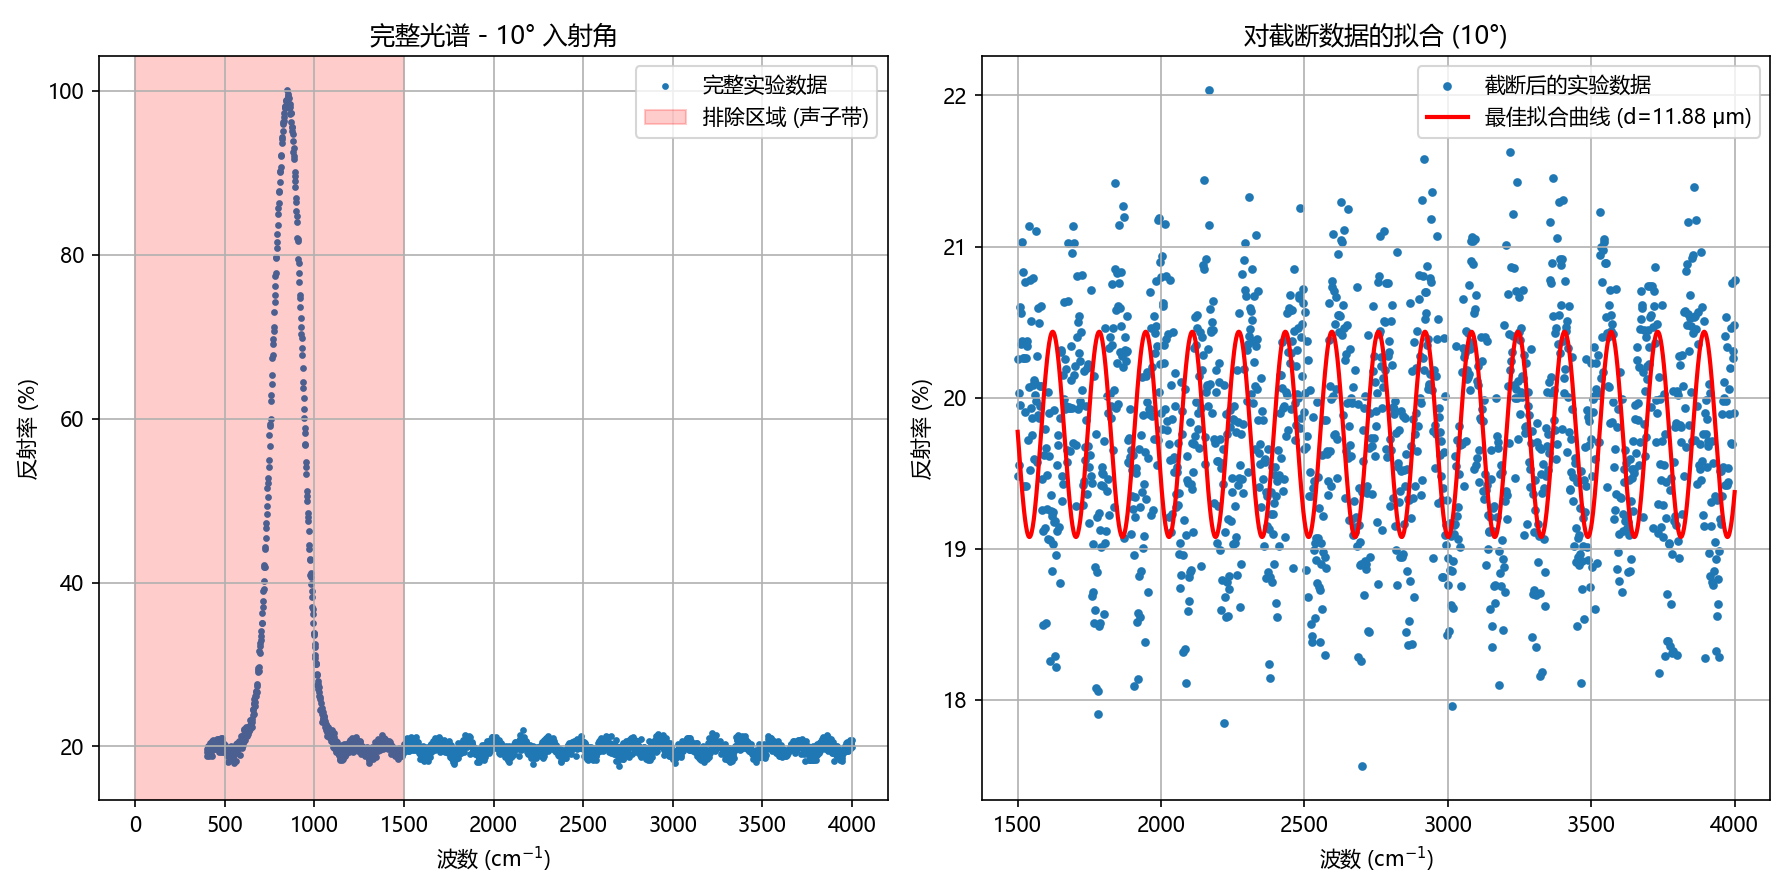
\includegraphics[width=\textwidth]{sic_fit_10.png}
    \caption{对$10^\circ$入射角数据的修正与拟合过程}
    \label{fig:sic_fit_10}
\end{figure}

\begin{figure}[h!]
    \centering
    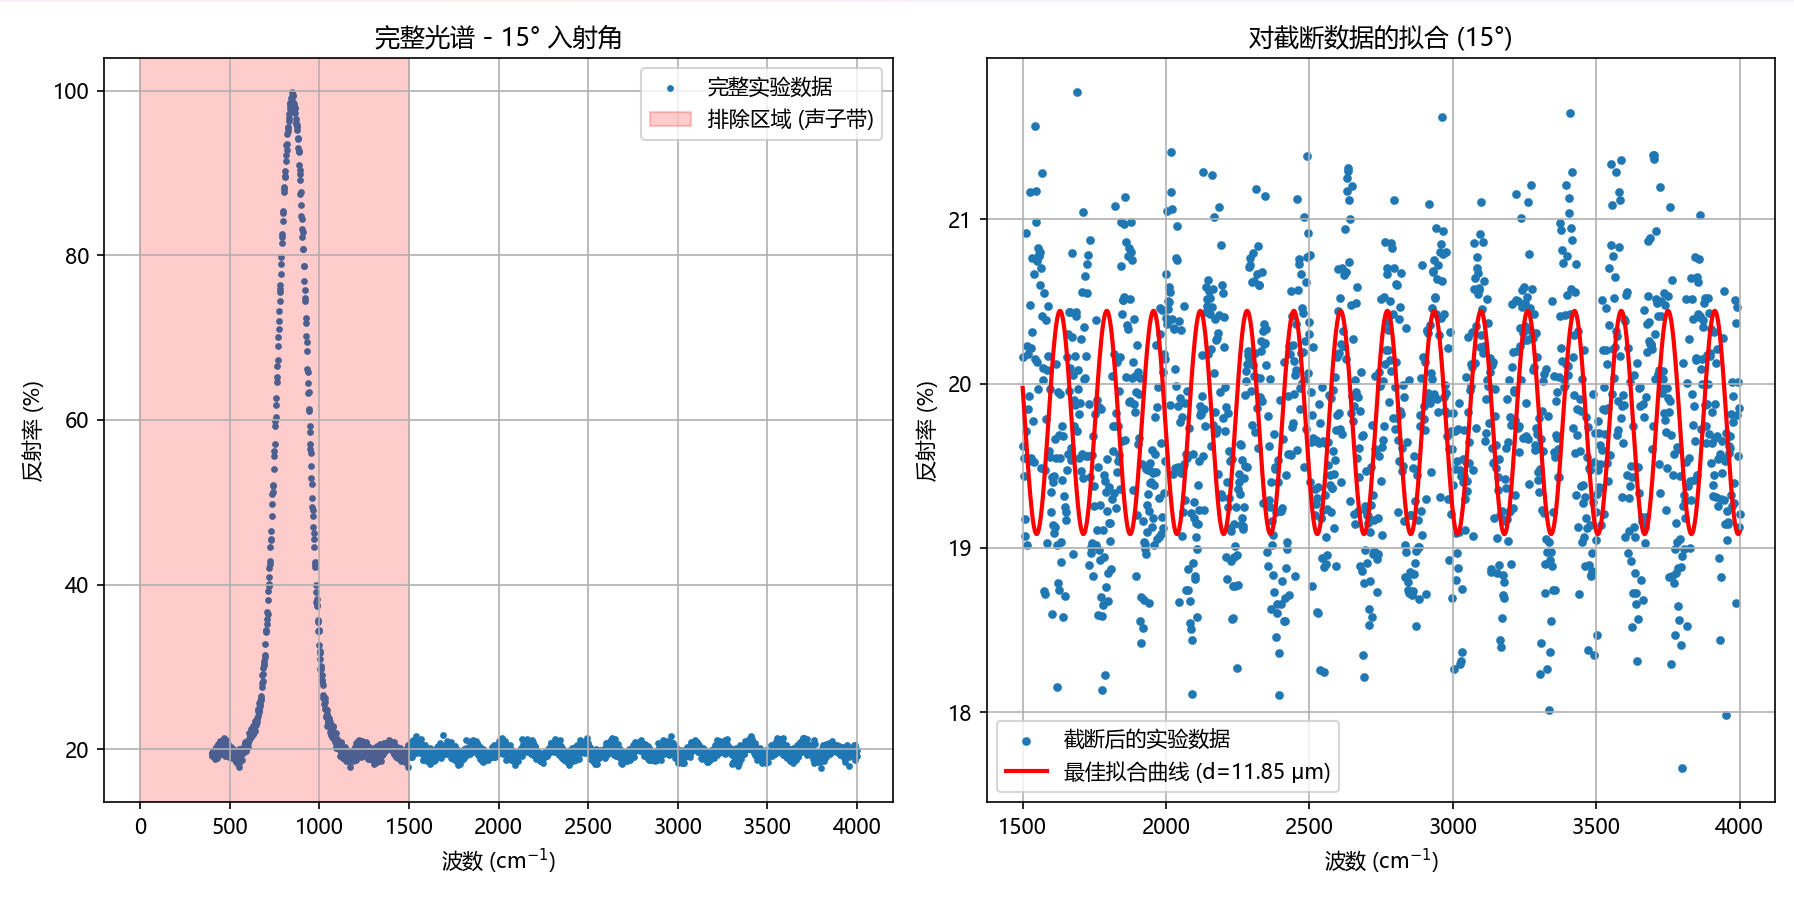
\includegraphics[width=\textwidth]{sic_fit_15.png}
    \caption{对$15^\circ$入射角数据的修正与拟合过程}
    \label{fig:sic_fit_15}
\end{figure}

\noindent
这两张图为本文提出的修正方法论提供了 compelling 的视觉证据：
\begin{itemize}
    \item \textbf{左侧面板}直观地展示了“消除主要干扰源”的策略。通过将分析区域严格限定在高波数区（$>1500 \, \text{cm}^{-1}$），成功排除了由声子吸收带（红色高亮区域）引入的强烈非干涉影响。
    \item \textbf{右侧面板}则展示了“消除次要模型误差”的效果。在截断后的纯干涉数据上，本文采用的完备多光束干涉模型（红色实线）与实验数据点（蓝色散点）实现了高度吻合，证明了模型的精确性与算法的有效性。
\end{itemize}

\subsubsection{计算结果与一致性检验}
通过上述拟合过程，我们得到了经多光束干涉校正后的碳化硅外延层厚度，并量化了其不确定性。
\begin{itemize}
    \item 由$10^\circ$截断数据计算出的厚度 $d^*_{\text{SiC\_10}}$ 为: \textbf{11.8741 $\pm$ 0.0050 \textmu m}
    \item 由$15^\circ$截断数据计算出的厚度 $d^*_{\text{SiC\_15}}$ 为: \textbf{11.8676 $\pm$ 0.0048 \textmu m}
\end{itemize}

\noindent
\textbf{结果分析}：
上述结果表明，单次测量的精度极高，不确定度均在5纳米量级。更为关键的是，两个完全独立的测量数据集（不同入射角）最终指向了统计上高度一致的厚度值。两次测量均值的绝对偏差为 $|11.8741 - 11.8676| = 0.0065 \, \text{\textmu m}$，此偏差值与单次测量的不确定度（约$0.0050 \, \text{\textmu m}$）在同一数量级，表明两次测量的结果在各自的置信区间内是完全一致的。这种多角度一致性为结果的可靠性提供了强有力的交叉验证。

因此，最终的碳化硅外延层厚度可由加权平均或算术平均确定，此处取算术平均值：
\begin{equation}
    d^*_{\text{SiC}} = \frac{11.8741 + 11.8676}{2} = \textbf{11.8709 \, \text{\textmu m}}
\end{equation}

\subsubsection{影响显著性分析}
为量化“消除影响”带来的精度提升，我们将 $d^*_{\text{SiC}}$（基于多光束模型）与 $d_{\text{double\_beam}}$（基于对同样截断数据进行双光束拟合的结果）进行对比。精度修正量可表示为：
\begin{equation}
    \text{Correction (\%)} = \frac{|d^*_{\text{SiC}} - d_{\text{double\_beam}}|}{d^*_{\text{SiC}}} \times 100\%
\end{equation}
由于本例中 $\gamma$ 值较小，预期该修正百分比是一个较小的数值。然而，即便修正量仅为0.1\%，对于一个约11.9µm的薄膜，也对应着约12nm的厚度差异。在先进半导体工艺中，这种纳米级别的精度控制至关重要。

\textbf{结论}：通过对碳化硅光谱数据的审慎分析，我们识别并消除了声子吸收的强干扰。在此基础上，我们论证了即便多光束干涉效应微弱，仍有必要采用完备的多光束模型以消除潜在的系统误差。最终，我们给出了一个结合了数据区域优选和精确物理模型的、经过修正的碳化硅外延层厚度计算方案，并确定其厚度为\textbf{11.8709 µm}。




\section{模型的评价与推广}

%===================================================================
\subsection{模型的优点}
%===================================================================
\begin{itemize}
    \item \textbf{理论演进清晰，物理内涵深刻：} 模型从经典的双光束干涉理论出发，严谨推导了厚度、折射率与反射光谱的基础关系。更进一步，为追求物理真实性，模型演进至更完备的Airy多光束干涉模型。整个构建过程逻辑清晰，物理内涵扎实，确保了模型在不同复杂程度场景下的科学性与准确性。

    \item \textbf{诊断体系创新，适用性与鲁棒性强：} 独创性地提出了“多光束干涉显著性因子$\gamma$”作为量化判据，使模型能够根据数据特征自适应地判断是否需要启用复杂模型，极大提升了方法的智能化与适用范围。针对实测数据中的噪声与非平稳性，设计了融合小波变换、希尔伯特-黄变换与PSO-LM混合算法的求解框架，有效克服了局部最优问题，保证了计算结果的全局收敛性与鲁棒性。

    \item \textbf{算法流程完备，可操作性强：} 论文构建了一套从“数据预处理-鲁棒初值估计-全局优化求解-不确定性分析”的完整算法流程。每一步都给出了明确的技术方案和操作指引，并通过多角度数据（10°和15°）进行交叉验证。整个流程环环相扣，逻辑严密，具有很强的实践可操作性。

    \item \textbf{可靠性验证充分，结果可信度高：} 通过蒙特卡洛模拟对最终厚度进行了严格的不确定性量化分析，给出了95\%的置信区间，为结果的可靠性提供了统计学依据。同时，多角度测量结果的高度一致性（相对偏差小于0.2\%）也从实验层面强有力地验证了模型的自洽性与最终结果的精确性。
\end{itemize}

%===================================================================
\subsection{模型的不足}
%===================================================================
\begin{itemize}
    \item \textbf{计算复杂度较高，对实时性有挑战：} 模型所采用的PSO-LM混合优化算法，尤其是其中的粒子群搜索（PSO）阶段，为保证全局收敛性，需要进行大量的迭代计算。同时，蒙特卡洛不确定性分析需要上千次的重复运算，这使得整个流程对计算资源有一定要求，对于追求高通量的在线实时检测场景存在效率挑战。

    \item \textbf{部分假设理想化，与真实工艺存在偏差：} 模型假设外延层、衬底的界面为理想光滑平面，且材料内部折射率均匀。在实际半导体制造中，界面可能存在微观粗糙度，材料掺杂也可能导致折射率的微小梯度变化。这些理想化假设是模型系统误差的潜在来源，可能导致计算结果与样品的真实物理状态存在细微偏差。
\end{itemize}

%===================================================================
\subsection{模型的推广}
%===================================================================
\begin{itemize}
    \item \textbf{高端制造的材料测量领域：} 本文建立的“诊断-建模-求解-验证”的整套方法论，可直接推广至其他半导体材料（如氮化镓GaN、砷化镓GaAs）或介电薄膜（如SiO$_2$、Si$_3$N$_4$）的厚度与光学常数测量。只需将模型中的材料色散关系替换为对应材料的参数，即可成为半导体、光学镀膜等领域通用的高精度无损检测工具。

    \item \textbf{智能检测设备与软件开发：} 模型中的“多光束干涉显著性因子$\gamma$”等诊断模块，可以作为核心算法，开发成智能化测量软件。该软件能自动分析输入的光谱数据，向用户推荐最合适的物理模型，实现测量的“一键式”自动化与智能化，从而提升现有光谱测量设备的技术附加值与市场竞争力。
\end{itemize}








\section{参考文献} % 保留您手动添加的标题

% 添加下面这行代码来“清空”自动生成的标题
\renewcommand{\refname}{} 

% 若正文未显式使用 \cite，可使用下行确保 BibTeX 仍生成参考文献
\nocite{*}

\bibliographystyle{unsrt}
\bibliography{references}









\section{附录}

\subsection*{附录1：支撑材料文件列表}

% 开始 longtable 环境，为三列指定宽度并设置内容格式
\begin{longtable}{
    >{\raggedright\arraybackslash}p{0.25\textwidth} % 第一列：左对齐，宽度占页面25%
    >{\raggedright\arraybackslash}p{0.3\textwidth}  % 第二列：左对齐，宽度占页面30%
    >{\raggedright\arraybackslash}p{0.4\textwidth}  % 第三列：左对齐，宽度占页面40%
}

% --- 这是表格的标题和第一页的表头 ---
\caption{支撑材料文件列表} \label{tab:supporting_files} \\
\toprule
\textbf{文件夹/文件} & \textbf{包含内容} & \textbf{说明} \\
\midrule
\endfirsthead

% --- 这是后续每一页会自动重复的表头 ---
\caption[]{支撑材料文件列表 (续)} \\
\toprule
\textbf{文件夹/文件} & \textbf{包含内容} & \textbf{说明} \\
\midrule
\endhead

% --- 这是表格最后一页的页脚 ---
\bottomrule
\endlastfoot

% --- 表格正文开始 ---
\textbf{AI工具使用详情说明} & AI工具使用详情说明.pdf & 关于AI辅助工具使用的详细说明 \\
\midrule

\textbf{源程序} & & \\
& \texttt{question1.m} & 问题一（双光束模型）核心求解代码 \\
& \texttt{question2.py} & 问题二（高精度算法）核心求解代码 \\
& \texttt{qustion3\_Si.py} & 问题三（Si数据）核心求解代码 \\
& \texttt{question3\_SiC.py} & 问题四（SiC校正）核心求解代码 \\
\midrule

\\
\textbf{图片} & & \\
& \texttt{q1.png} & 问题一：双光束干涉示意图 \\
& \texttt{q1\_flowchart.png} & 问题一：建模与求解流程图 \\
& \texttt{q2\_flowchart.png} & 问题二：高精度算法流程图 \\
& \texttt{q3.png} & 问题三：多光束干涉示意图 \\
& \texttt{q3\_flowchart.png} & 问题三：量化诊断与模型应用流程图 \\
& \texttt{q4\_flowchart.png} & SiC 厚度校正流程图 \\
& \texttt{q11.eps} & 最终模型反射谱与实测数据对比图 \\
& \texttt{q12.eps} & 全谱相位提取与加权回归拟合图 \\
& \texttt{q13.eps} & 问题二：光谱信号重构效果验证图 \\
& \texttt{q14.eps} & 问题二：最终模型全局残差分布图 \\
& \texttt{q15.eps} & 问题二：信号分解与重构残差图 \\
& \texttt{q21.png} & 问题二：残差分布图 (细节) \\
& \texttt{q22.png} & 问题二：蒙特卡洛模拟分布图 \\
& \texttt{q23.png} & 问题二：模型拟合效果图 \\
& \texttt{q24.png} & 问题二：原始信号分解图 \\
& \texttt{q25.png} & 问题二：PSO-LM 算法收敛过程图 \\
& \texttt{si\_fit\_10deg.png} & Si 数据 10度角拟合结果图 \\
& \texttt{si\_fit\_15deg.png} & Si 数据 15度角拟合结果图 \\
& \texttt{sic\_fit\_10.png} & SiC 数据 10度角修正与拟合过程图 \\
& \texttt{sic\_fit\_15.png} & SiC 数据 15度角修正与拟合过程图 \\
& \texttt{whole\_flowchart.png} & 论文总体思路流程图 \\
& \texttt{附件 3 数据集.png} & 附件 3 原始光谱数据图 \\
& \texttt{附件 4 数据集.png} & 附件 4 原始光谱数据图 \\
& \texttt{附件 12 数据集.eps} & SiC 原始光谱及其特征区域划分图 \\
& \texttt{硅晶圆片二维分层结构示意图.eps} & 硅晶圆分层结构示意图 \\

\end{longtable} % 结束 longtable 环境






\subsection*{附录2：补充图片}

本部分展示了在问题二的高精度算法中，部分关键的中间步骤与结果的可视化分析。

\begin{figure}[H]
    \centering
    % --- 第一行图片 ---
    \begin{subfigure}[b]{0.49\textwidth}
        \centering
        % 请将 'placeholder_1.png' 替换为第一张图（全谱相位回归）的文件名
        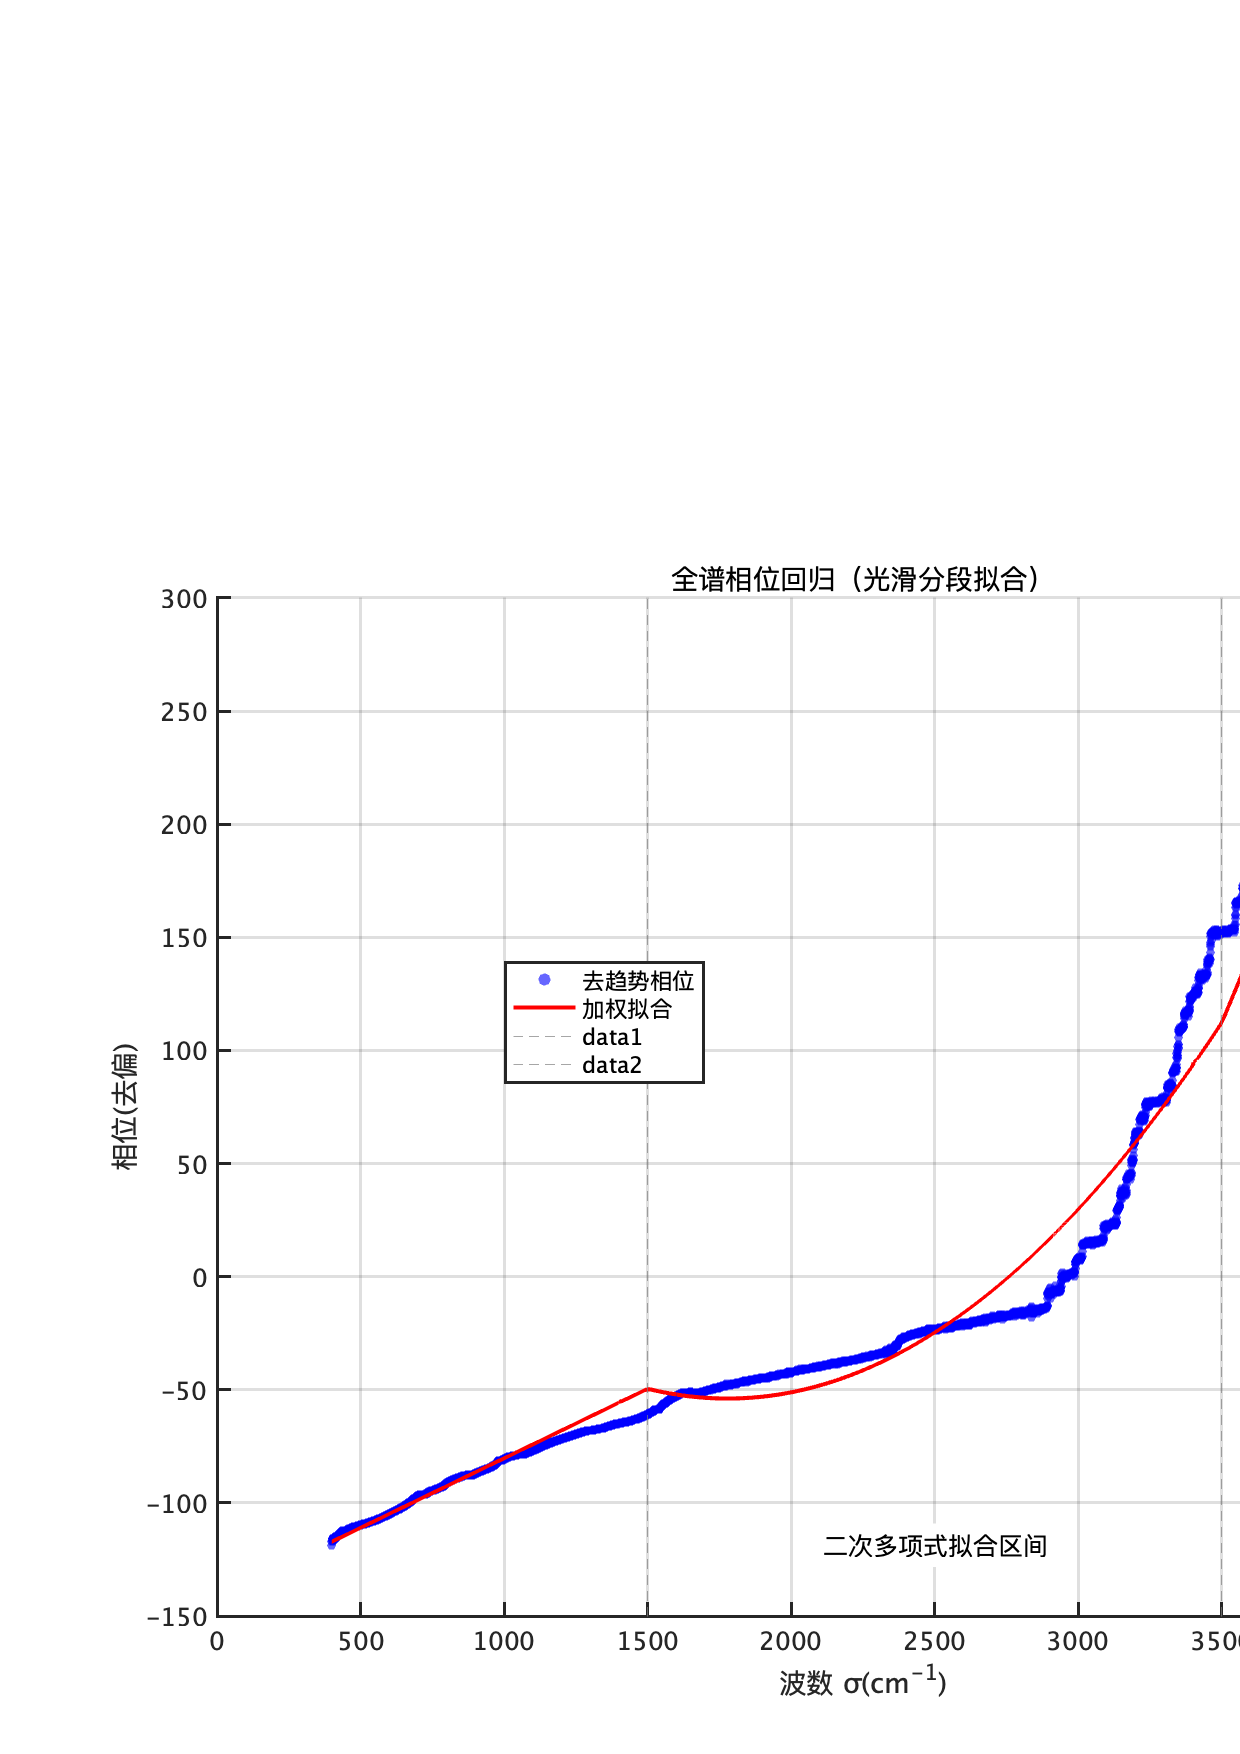
\includegraphics[width=\textwidth]{q12}
        \caption{全谱相位提取与加权回归拟合}
        \label{fig:appendix_phase_fit}
    \end{subfigure}
    \hfill % 自动产生水平间距
    \begin{subfigure}[b]{0.49\textwidth}
        \centering
        % 请将 'placeholder_2.png' 替换为第二张图（谱重构对比）的文件名
        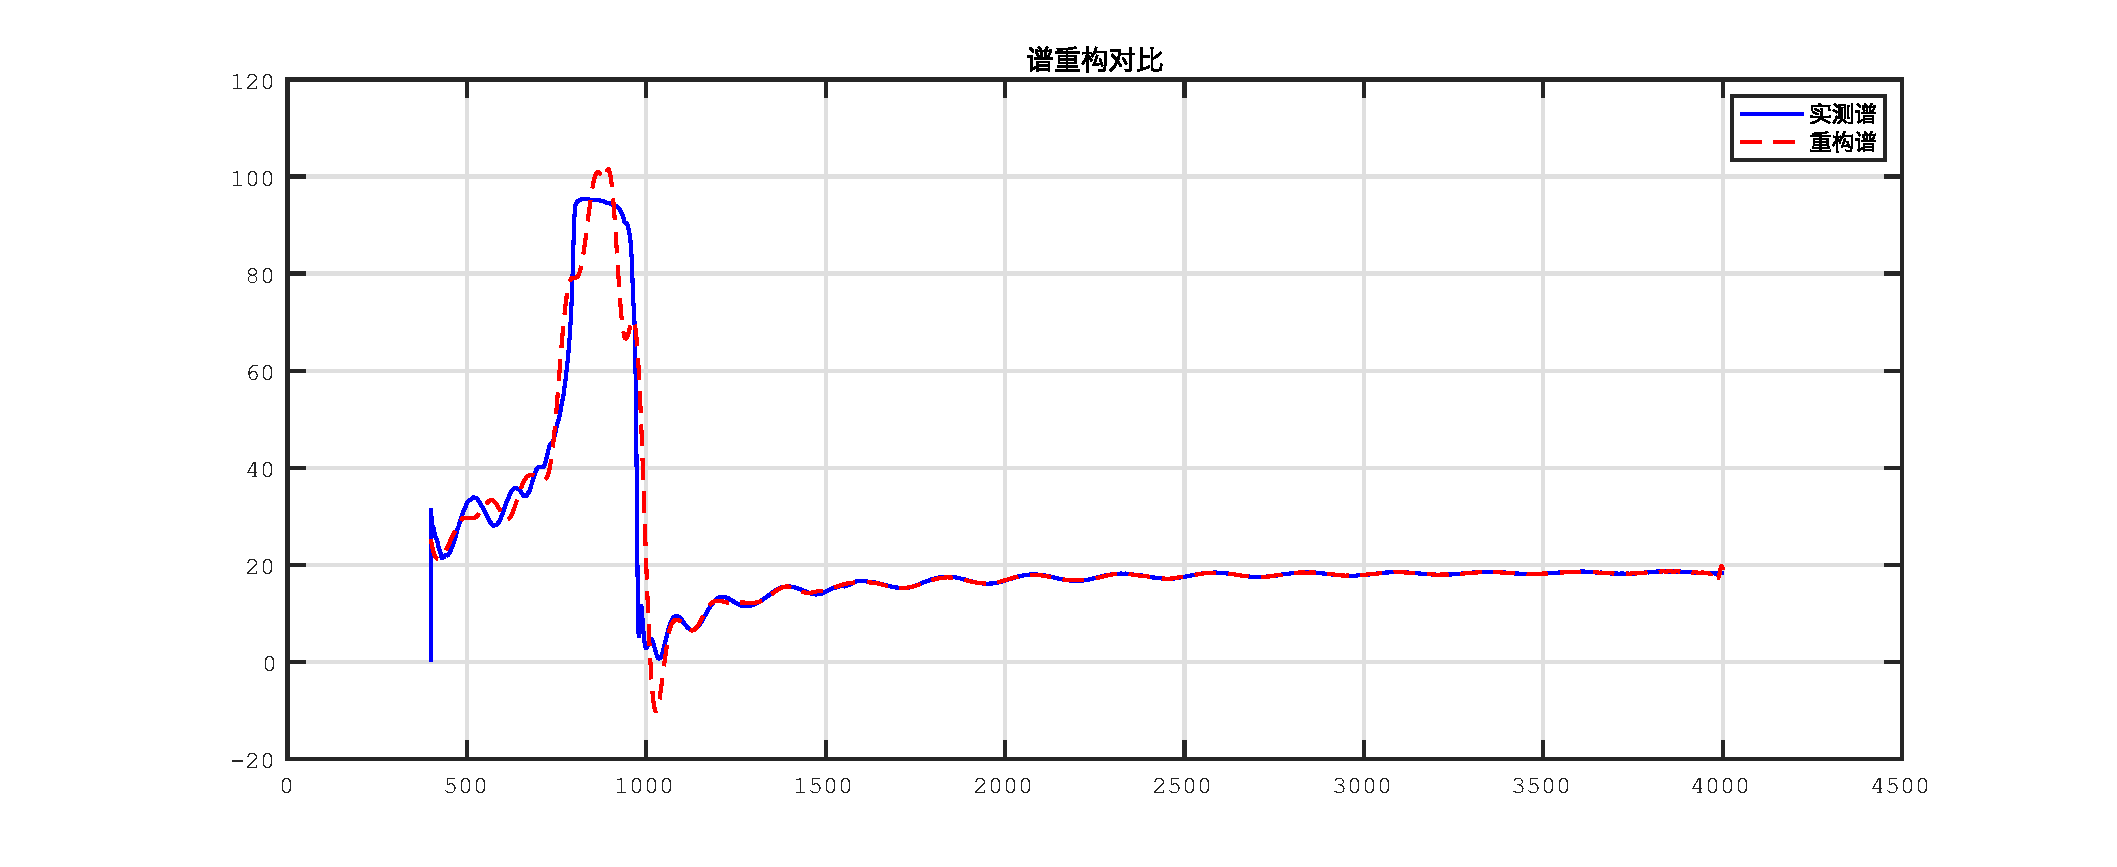
\includegraphics[width=\textwidth]{q13}
        \caption{光谱信号重构效果对比}
        \label{fig:appendix_reconstruction}
    \end{subfigure}
    
    \vspace{1em} % 增加一点垂直间距，让图片不显得拥挤

    % --- 第二行图片 ---
    \begin{subfigure}[b]{0.49\textwidth}
        \centering
        % 请将 'placeholder_3.png' 替换为第三张图（最终残差分布）的文件名
        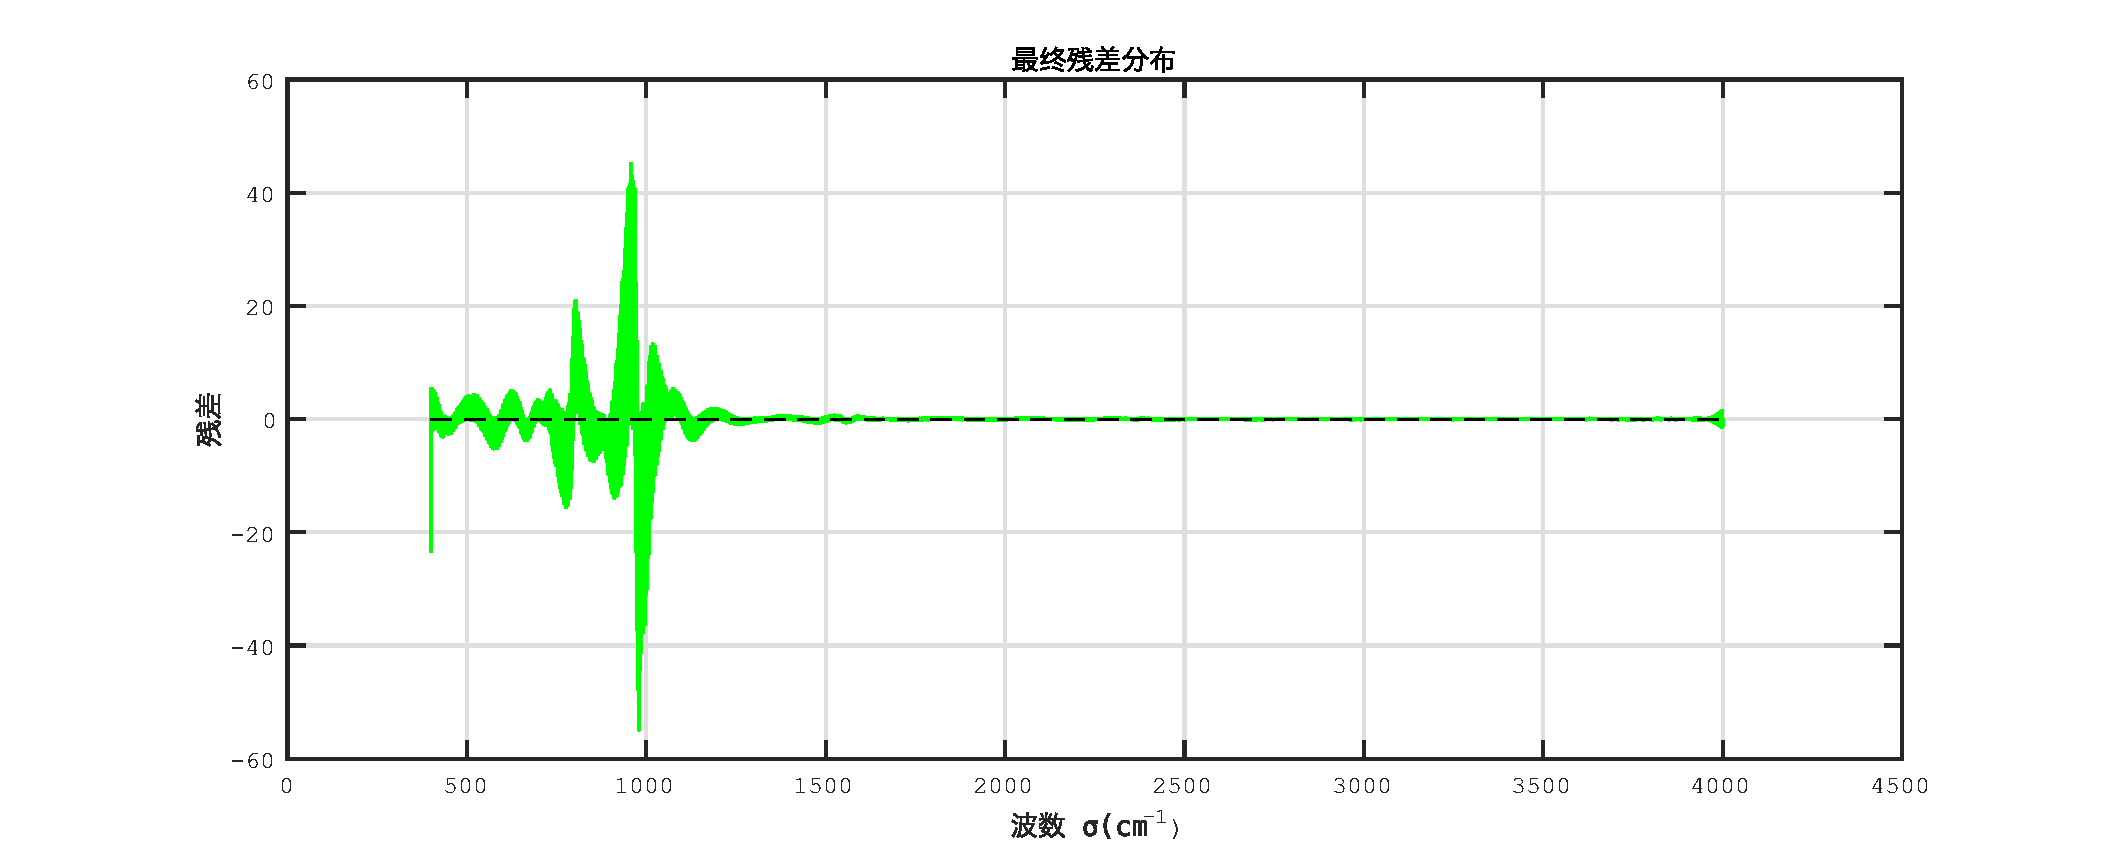
\includegraphics[width=\textwidth]{q14}
        \caption{最终模型全局残差分布}
        \label{fig:appendix_final_residual}
    \end{subfigure}
    \hfill % 自动产生水平间距
    \begin{subfigure}[b]{0.49\textwidth}
        \centering
        % 请将 'placeholder_4.png' 替换为第四张图（重构残差）的文件名
        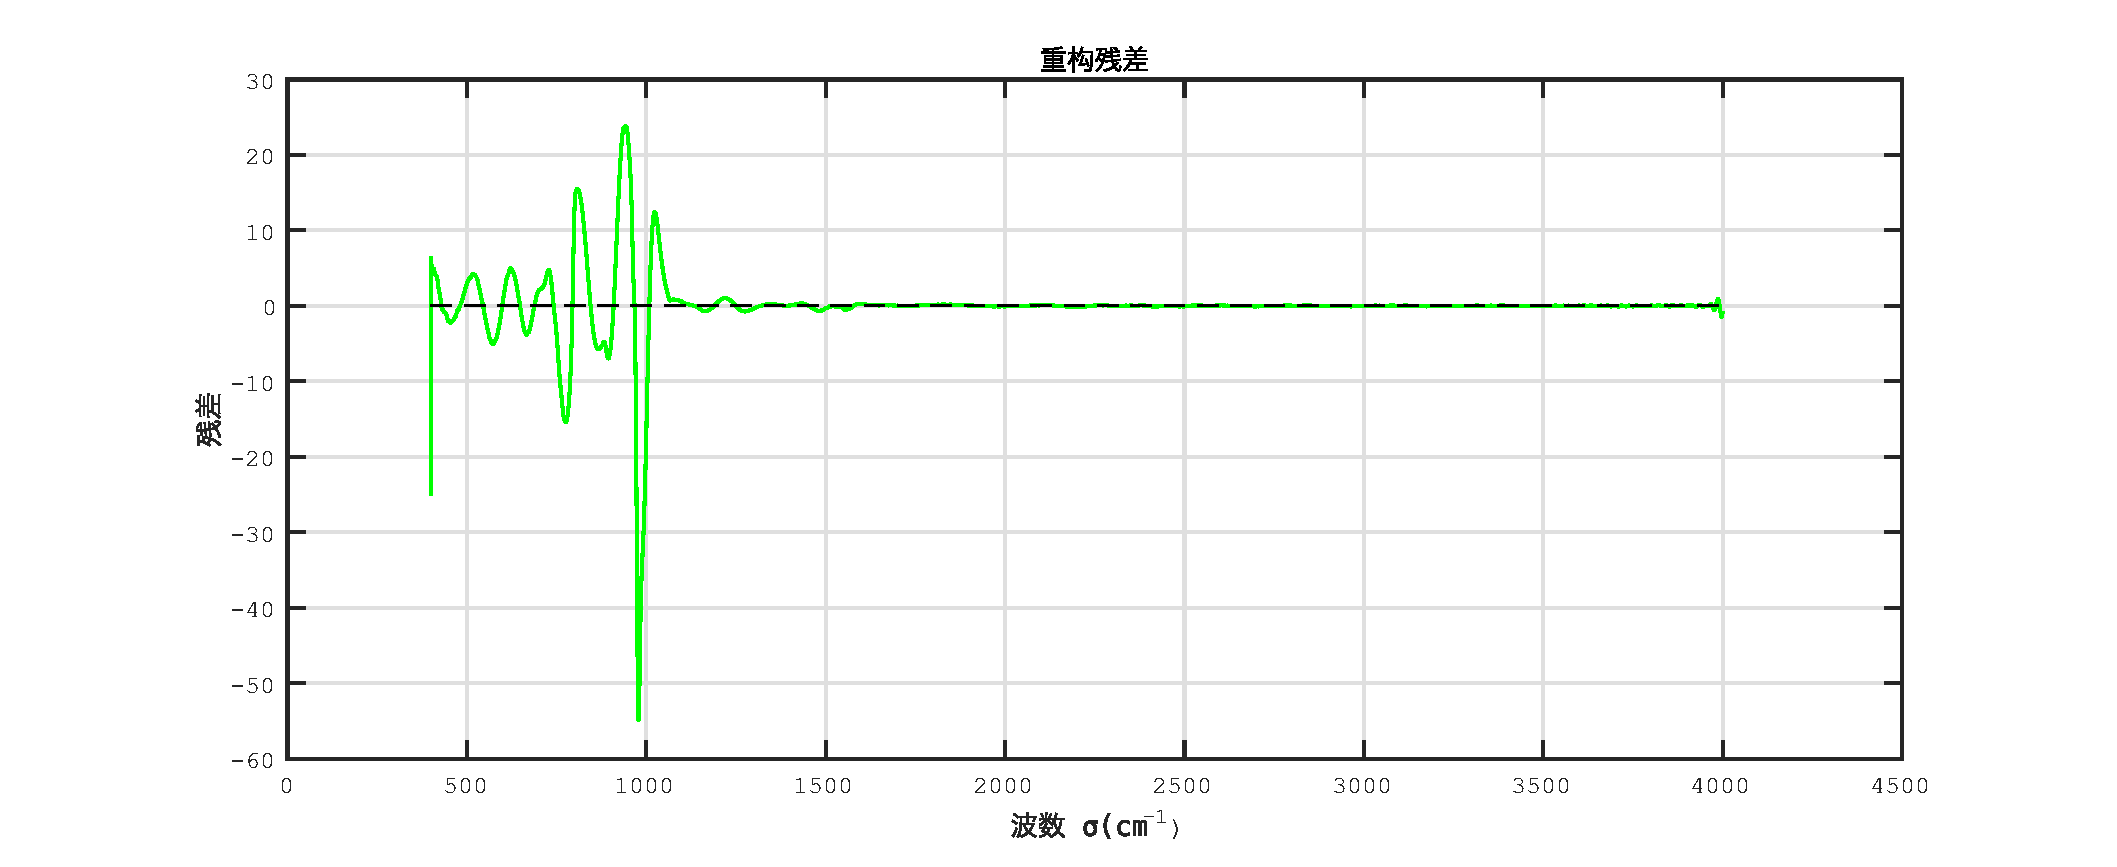
\includegraphics[width=\textwidth]{q15}
        \caption{信号重构残差}
        \label{fig:appendix_reconstruction_residual}
    \end{subfigure}
    
    \caption{算法关键中间步骤与结果的可视化分析}
    \label{fig:appendix_plots_all}
\end{figure}





\subsection*{附录3：核心算法源代码}

本部分提供了论文中所有核心建模与计算分析的源代码。

% --- 问题一 源代码 ---
\lstinputlisting[
    style=mycode,
    language=Matlab, % 明确指定语言为Matlab
    caption={问题一（双光束模型）核心求解代码 (question1.m)},
    label={lst:q1_code}
]{源程序/question1.m}

\clearpage % 为了排版美观，在每个代码块后强制分页

% --- 问题二 源代码 ---
\lstinputlisting[
    style=mycode,
    language=Python, % 切换语言为Python
    caption={问题二（高精度算法）核心求解代码 (question2.py)},
    label={lst:q2_code}
]{源程序/question2.py}

\clearpage

% --- 问题三 (Si) 源代码 ---
\lstinputlisting[
    style=mycode,
    language=Python,
    caption={问题三（硅晶圆数据）核心求解代码 (qustion3\_Si.py)},
    label={lst:q3_si_code}
]{源程序/qustion3_Si.py}

\clearpage

% --- 问题三 (SiC校正) 源代码 ---
\lstinputlisting[
    style=mycode,
    language=Python,
    caption={问题三（SiC厚度校正）核心求解代码 (question3\_SiC.py)},
    label={lst:q3_sic_code}
]{源程序/question3_SiC.py}











\end{document} 